\documentclass{ruthesis}
\special{papersize=8.5in,11in} % for A4-default configurations on servers


\usepackage[utf8]{inputenc}
\usepackage{longtable}
\usepackage{graphicx}
\usepackage{amssymb,amsmath,amsfonts}
\usepackage{amsbsy}
\usepackage[utf8]{inputenc}
\usepackage{array}
\usepackage{booktabs}
\usepackage{algorithm2e}
\usepackage{listings}
\usepackage{cleveref}
\usepackage{acronym}
\usepackage{subcaption}

\acrodef{QoS}{Quality of Service}
\acrodef{VM}{Virtual Machine}
\acrodef{UDF}{User Defined Function}
\acrodef{DAG}{Directed Acyclic Graph}
\acrodef{CEP}{Complex Event Processing}
\acrodef{IoT}{Internet of Things}
\acrodef{DSPE}{Data Stream Processing Engine}
\acrodef{DSP}{Data Stream Processing}
\acrodef{FCFS}{First-Come, First-Served}
\acrodef{SPDG}{Series-Parallel-Decomposable Graphs}
\acrodef{IPS}{Instructions per Second}
\acrodef{RTR}{Response Time Rate}
\acrodef{CR+RP}{Cost Rate with Region Patterns}
\acrodef{CI}{Cloud Infrastructure}
\acrodef{EI}{Edge Infrastructure}
\acrodef{LB}{Taneja et. al.}
\acrodef{DSP}{Distributed Stream Processing}
\acrodef{MIPS}{Millions of Instructions per Second}
\acrodef{SDN}{Software Defined Network}
\acrodef{SoC}{System on a Chip}
\acrodef{CDF}{Cumulative distribution function}
\acrodef{OODA}{Observe Orient Decide Act}

% set the default code style
\lstset{
    frame=tb, % draw a frame at the top and bottom of the code block
    tabsize=1, % tab space width
    showstringspaces=false, % don't mark spaces in strings
    basicstyle=\small,
    keywordstyle=[1]\color{green},
    keywordstyle=[2]\color{orange},
    keywordstyle=[3]\color{blue},
}

\lstdefinelanguage{mylang}{
  alsoletter={*,", 10, >=, :, 74,40,-},
  keywords=[1]{placement, minEndToEndLatency, minDataTransferRate, minMessagingCost},
  keywords=[2]{core, edge, *},
  keywords=[3]{new},
}

\begin{document}
\phd

%\title{Enabling Data-driven Stream Processing Pipelines for Edge Computing}
\title{Programming and Managing stream processing applications between the edge and the cloud}
\author{Eduard Gibert Renart}
\program{Computer Science}
\director{Manish Parashar}
\approvals{4}
\submissionyear{2017}
\submissionmonth{May}

\abstract{Due to the proliferation of the Internet of Things (IoT), the number of devices connected to the Internet is growing. These devices are generating unprecedented amounts of data at the edge of the infrastructure. Although the generated data provides great potential, identifying and processing relevant data points hidden in streams of unimportant data, and doing this in near real time, remains a significant challenge. Existing stream processing platforms require the data to be transported to the cloud for processing, resulting in latencies that can prevent timely decision making or may reduce the amount of data processed.


To address these challenges, this dissertation presents an IoT Edge Framework, called R-Pulsar, that extends cloud capabilities to local devices and provides a programming model for deciding what, when, where and how data get collected and processed. This thesis makes the following contributions: (1) A content- and location-based programming abstraction for specifying \textbf{what} data gets collected and \textbf{where} the data gets analyzed. (2) A rule-based programming abstraction for specifying \textbf{when} to trigger data-processing tasks based on data observations. (3) A programming abstraction for specifying \textbf{how} to split a given dataflow and place operators across edge and cloud resources. (4) An operator placement strategy that aims to minimize an aggregate cost which covers the end-to-end latency (time for an event to traverse the entire dataflow), the data transfer rate (amount of data transferred between the edge and the cloud) and the messaging cost (number of messages transferred between edge and the cloud). (5) Performance optimizations on the data-processing pipeline in order to achieve real-time performance on constrained devices.

The applicability of this work to real-world IoT applications is validated through a series of experiments where 

heterogeneous, geographically distributed services are composed based on user, resource provider, and application specifications. The results establish the potential impact of a system capable of real-time adaptability to changes in mixed resource environments, including multiple clouds, grids, clusters, supercomputers, and traditional data centers.



(6) An implementation of the above capabilities as part of the R-Pulsar software stack and its evaluation using embedded devices (Raspberry Pi and Android phone)}

\beforepreface
\acknowledgements{The body of the acknowledgements}
\dedication{The body of the dedication}
\afterpreface

\listoftables
\listoffigures

\chapter{Introduction}
%\hl{Internet of Things (IoT) refers to a system of connected physical objects via the internet. The 'thing' in IoT can refer to a person or any device which is assigned through an IP address. A 'thing' collects and transfers data over the internet without any manual intervention with the help of embedded technology. It helps them to interact with the external environment or internal states to take the decisions.}

%The proliferation of the Internet of Things (IoT) is fostering the connection of massive numbers of devices to the network. It is predicted that by 2020 there will be 50 to 100 billion devices connected to the Internet and constantly producing data[].

%IoT analytics refers to the analysis of data from multiple IoT data sources, including sensors, actuators, smart devices and other internet connected objects. The collection and analysis of data streams from IoT sources is nowadays considered a key element of the IoT’s disruptive power, as well as a prerequisite to realizing IoT’s hyped market potential. Indeed, according to a recent report by McKinsey[], less than 1\% of IoT data is currently used, which is a serious set-back to maximizing IoT’s business value. For example, most IoT analytics applications are nowadays used for anomaly detection and control rather than for optimization and prediction, which are the applications that will provide the greatest business value in the coming years.

%\section{IoT Data and BigData}

%\hl{Big data means a large set (petabytes or gigabytes) of structured, unstructured or semi-structured data and analyzing those data to get the insights of the business trend.}


%\section{Challenges of IoT Applications}

%Internet of Things(IoT) and big data are closely intertwined and although they are not the same thing.
%The term big data existed long before IoT arrived. When the information demonstrates veracity, velocity, variety and volume, then it is interpreted as big data

%IoT data is essentially BigData since they feature several of the Vs of BigData, including
%\begin{itemize}
%    \item Volume: IoT data is machine-generated data coming from a wide variety of sensors, where big data is mostly human-generated data.
%    \item Velocity: Refers to the speed data is being produced, collected and analyzed. IoT, data needs to ingest hundreds of thousands, or even millions, of events per second from their devices.
%    \item Variety: Since IoT encompasses a large variety of IoT devices, IoT data can be very heterogeneous both in terms of semantics and data formats.
%    \item Veracity: Several IoT streams are noisy and incomplete, which creates uncertainty in the scope of IoT analytics applications. Statistical and probabilistic approaches must be therefore employed in order to take into account the noisy nature of IoT data streams, especially in cases where they stem from unreliable sensors.
%\end{itemize}

%IoT data differ from big data datasets and introduces new challenges, this are some of the new characteristics that IoT introduces:

%\begin{itemize}
%    \item Data heterogeneity:
%    \item Real-time nature: While in big data projects it is perfectly normal for data to rest before it is used in any kind of analysis, in any IoT projects time is of the absolute essence, for several application must be processes nearly in real-time.
%    \item Time and location dependencies: IoT data is naturally geo-distributed and generated at the edge of the network, sometimes involving fast moving sensors. Big data is mostly generated from a single location, the core of the network.
%    \item Privacy and security sensitivity:
%\end{itemize}

%\section{IoT Application Lifecycle}
%The IoT application lifecycle comprises of the following three phases: Data Collection, Data Analysis and Data Storage and Query.

%\begin{enumerate}
%\item \textbf{Data collection:} gathers data from multiple sources and brings them to the pipeline.
%\item \textbf{Data Analysis:} processes the data and performs computations on the collected data.   
%\item \textbf{Data Storage and Query:} reads and writes data to the main memory and disk.
%\end{enumerate}

The Internet of Things (IoT) is an emerging concept that is fostering the connection of massive numbers of objects, sensors, and devices to the network. As per Cisco systems\footnote{Cisco, Internet of Things At-a-Glance, 2016 }, 500 billion devices are expected to be connected the Internet by 2030, and nearly half of the worldwide data will come from sensors~\cite{McAuley}. 
%
IoT devices produce important and timely data that can lead to new and transformative applications that are important to science and society, such as:
%
\begin{itemize} 
  \item Precision medicine applications that benefit from runtime actuation based on continuous monitoring by scientific instruments.
  \item Urban mobility applications that rely on processing data from sensors to identify and alleviate traffic congestion. 
  \item Healthcare applications that infer lifestyle patterns based on behavioral information obtained from wearables. 
\end{itemize} 

Making such applications a reality requires collecting data from sensors and instruments, processing this data individually or collectively in a timely manner, and making decisions based on the results. 

Stream processing frameworks (SPFs) have proven to be very effective at processing large amounts of data at near-real time, especially when combined with the elasticity and scalability of the cloud. Nonetheless, existing solutions were developed keeping in mind Big Data streams generated at the core of the infrastructure, such as those associated with web analytics. As a result, applying these solutions to IoT data stream requires transferring data from the edges to a data center located at the core of the infrastructure for processing. The prevalent model of moving data located at the edge of the network to the core of the network to process is quickly becoming unsustainable~\cite{intro}. The resulting impact on latency, network congestion, storage cost, and privacy can limit the potential impact of IoT.

However, in recent years, non-trivial computational capabilities have proliferated across the computing service landscape~\cite{continuum}. In particular, edge services are emerging close to the data sources and can provide potential data-processing capabilities\cite{dastjerdi2016fog,bonomi2014fog}. Furthermore, not all the data produced is interesting or relevant, and only a part of it may need to be processed in the context of an application. These observations can be leveraged to design hybrid architectures that can effectively leverage both the edge and the cloud resources to process the data in an effective and timely manner\cite{ahmed2017role, satyanarayanan2015edge}.

Although the cloud is better suited to perform heavier (resource intensive) analysis, such as processing historical events and very large datasets, edge devices can support real-time analytics that consider the temporal, spatial, and continuous nature of IoT data. 

While such edge-based data processing can benefit IoT applications, edge resources are typically constrained in their capabilities. Therefore, the edge resources can be leveraged to complement the computing capabilities of the cloud-centric approach and reduce the overall latency and bandwidth requirements. The use of the edge and cloud architecture poses the following challenges: 

\begin{itemize}
\item Deciding how to split such IoT applications among the edge and cloud resources;

\item Exploring heterogeneous infrastructure for deploying dataflow applications has proved to be NP-hard \cite{Benoit:2013}.
 
\item Moving operators from cloud to edge devices is challenging due to the devices' limitations with respect to memory, CPU, and often network bandwidth \cite{dias:2018:survey}.
\end{itemize}

Solving the challenges presented above in a correct manner will allow for faster completion time, a reduction in edge to cloud data transfers, and ensure an efficient use of the edge and cloud resources. Doing them incorrectly can be detrimental to throughput and exacerbate the time for handling data events.
 
Such flexibility is not currently offered in state-of-the-art IoT systems or stream processing engines. Major systems, such as Azure IoT~\cite{azure}, AWS Greengrass~\cite{amazon}, and IBM Watson IoT~\cite{IBM}, do not offer programming support for orchestrating the execution of data-processing tasks between the cloud and the edge. Therefore, the developers' ability to specify ``What data needs to be processed?,'' ``Where to deploy the computations?,'' and ``When to deploy the computations?,'' is limited. Moreover, existing IoT stacks tend to perform poorly when deployed on constrained devices, making it nearly impossible to support real-time data analytics on these devices.


\section{Motivation}

Due to the proliferation of the Internet of Things (IoT) paradigm, the number of devices connected to the Internet is growing. These devices are generating unprecedented amounts of data at the edges of the infrastructure. As per Cisco systems\footnote{Cisco, Internet of Things At-a-Glance, 2016 }, 500 billion devices are expected to be connected the Internet by 2030. Consequently, the volume of data generated by this devices will increase, along with the volume of network traffic to the cloud thereby resulting in latencies that can prevent timely decision making or may reduce the amount of data processed.


The popularity and proliferation of the Internet of Things (IoT) paradigm is resulting in a growing number of devices connected to the Internet. These devices are generating and consuming unprecedented amounts of data at the edges of the infrastructure, and are enabling new classes of applications, however, current approaches typically rely on cloud
platforms located at the core of the infrastructure to process data. As the number of devices and the amount of data they generate and consume increases, such core-centric approaches are becoming increasingly inefficient as they need to transfer data back and forth between the edge and the core. Furthermore, the latencies associated with such data transfer may not be able to support applications involving time-critical data-driven decision making.


To address these limitations, we propose R-Pulsar, a software stack with a content- and location-based programming abstraction to perform and orchestrate data analytics between the edge and the cloud. The programming abstraction enables developers to address the \textbf{what}, \textbf{where}, and \textbf{when} data needs to be processed by specifying content and action descriptors. We also propose a programming model to provide developers with the ability to define \textbf{how} to automatically split the dataflow across the edge and the cloud by specifying a set of dataflow constraints. In addition we present an optimized data-processing pipeline for achieving real-time data analytics on constrained devices.

\section{Problem Description}

\section{Contributions}
The primary contributions of the research in this thesis are a programming model for deciding \textbf{what}, \textbf{when}, \textbf{where} data needs to be processed by specifying content and action descriptors and \textbf{how} computations get distributed across the edge and the cloud. The detailed contributions are presented as follows.
\begin{itemize}
  \item A content- and location-based programming abstraction for specifying \textbf{what} data gets collected and \textbf{where} the data gets analyzed.
  \item A rule-based programming abstraction for specifying \textbf{when} to trigger data-processing tasks based on data observations.
  \item A programming abstraction for specifying \textbf{how} to split a given dataflow and place operators across edge and cloud resources.
  \item An operator placement strategy that aims to minimize an aggregate cost which covers the end-to-end latency (time for an event to traverse the entire dataflow), the data transfer rate (amount of data transferred between the edge and the cloud) and the messaging cost (number of messages transferred between edge and the cloud).
  \item Performance optimizations on the data-processing pipeline in order to achieve real-time performance on constrained devices.
  \item An implementation of the above capabilities as part of the R-Pulsar software stack and its evaluation using embedded devices (Raspberry Pi and Android phone).
\end{itemize}

\section{Outline}

\begin{figure}[h!]
  \centering
  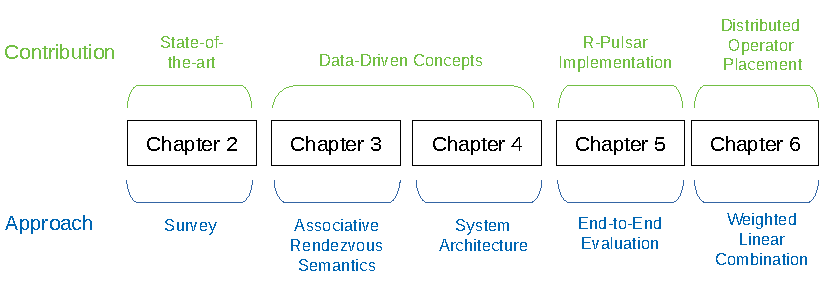
\includegraphics[width=1\textwidth]{Figures/Outline.pdf}
  \caption{Thesis Organization.}
  \label{fig:Outline}
\end{figure}

The core chapters of the thesis are structured as shown in Figure~\ref{fig:Outline} and are deviated from articles and journals published during the PhD. The remaining of the thesis is organized as follows: 

\begin{itemize}
    \item Chapter 2 shows the motivating use cases that where used to build R-Pulsar. 
    \item Chapter 3 presents an extensive literature review of related work. 
    \item Chapter 4 presents the programming abstraction that R-Pulsar builds upon.
    \item Chapter 5 presents the system concepts on what R-Pulsar was build upon. 
    \item Chapter 6 presents the implementation and evaluation details of R-Pulsar. 
    \item Chapter 7 introduces the operator placement problem. 
    \item Chapter 8 concludes the dissertation by outlining future research work.
\end{itemize}


\chapter{Motivating Applications and Requirements}
\section{Emergence, Benefits and Limitations of Using Edge Computing}
Edge computing complements the cloud in IoT by filling in the gap between the cloud and the internet of things by providing computing in the continuum. In this section we describe the advantages and disadvantages of Edge computing and later propose some IoT applications that will benefit from using edge computing.

\subsection{Advantages}

Minimize Data Explosion and Network Traffic: Due to the large number of connected devices the volume of data that they will generate will increase exponentially. Another concern with increasing data generation is the volume of network traffic to a central server or cloud thereby reducing the response time of edge devices. By using edge computing data can stay local and only send the important data to the cloud, reducing the volume and network bandwidth.

Low Latency: Emerging IoT scenarios involve gathering and processing large volumes of streaming data using complex workflows in a timely manner to support decision making. Traditionally, data processing has been done at large data centers in the core of the network, however, as the data volumes and rates grow, and the application scenario becomes increasingly time sensitive, such an approach is quickly becoming infeasible, and it is becoming essential to also leverage resources closer to the edge. By applying edge computing applications are capable of supporting time-sensitive applications.

Real-Time Computations: Edge computing improves the overall performance by offloading computations near the data source and reducing the unnecessary costs of moving the data to the cloud.

Security: Edge computing allows to process and filter sensitive data locally and transmit only the aggregate data over to the cloud.

\subsection{Disadvantages}
Limited Resources: While leveraging edge resources can alleviate costs associated with cloud data transfers, edge resources tend to be constrained in their capabilities. In addition state-of-the-art data analytics pipelines are known to be computationally intensive tasks, resulting in the inability to performing real-time data analytics when deployed on constrained devices.

Added complexity: Integrating edge computing adds complexity to applications, especially when they need to include policies that govern what kind of data is processed and analyzed at the edge and what is sent to cloud. In addition exploring heterogeneous infrastructures such as edge and cloud for deploying dataflow applications has proved to be NP-hard~\cite{Benoit:2013}.

Programmability: In cloud computing, users program their code and deploy them on the cloud. The cloud provider is in charge to decide where the computing is conducted in a cloud. Users have zero or partial knowledge of where the applications are running. However, in the edge computing, computation is offloaded from the cloud, and the edge nodes are most likely heterogeneous platforms. In this case, the runtime of these nodes differ from each other, and the programmer faces huge difficulties to write an application that may be deployed in the edge computing paradigm.

\begin{table*}[ht]
\caption{Edge Computing use cases, current limitations, and imperatives}
\label{tab:use_case}
\resizebox{\textwidth}{!}{%
\begin{tabular}{|c|c|c|c|}
\hline
Applications                                                                                    & Example Use Case                                                                                                                                                                              & Limitations                                                                                                                                                      & Requirements                                                                                                                                         \\ \hline
Smart City                                                                                      & \begin{tabular}[c]{@{}c@{}}Help autistic people \\ navigate through large \\ crowded spaces.\end{tabular}                                                                                     & \begin{tabular}[c]{@{}c@{}}Hard to provide real-time \\ directions due to the need to \\ send large volumes of data to \\ the cloud.\end{tabular}                & \begin{tabular}[c]{@{}c@{}}Low Latency, Security,\\ Geographically \\ Distributed,\\ Mobility, Scalability\\ Reliability and Robustness\end{tabular} \\ \hline
\begin{tabular}[c]{@{}c@{}}Disaster \\ Recovery\end{tabular}                                    & \begin{tabular}[c]{@{}c@{}}Need to quickly determine \\  whether  building conditions \\ are safe for  evacuees to return \\ after a natural  disaster \\ has struck.\end{tabular}            & \begin{tabular}[c]{@{}c@{}}Hard to perform real-time \\ decision due to the need to \\ send large volumes of data to \\ the cloud.\end{tabular}                  & \begin{tabular}[c]{@{}c@{}}Low Latency,\\ Geographically  \\ Distributed,\\ Orchestration \\ and Management\end{tabular}                             \\ \hline
\begin{tabular}[c]{@{}c@{}}Distributed \\ Observatories\end{tabular}                            & \begin{tabular}[c]{@{}c@{}}Large networked system of \\ under water instruments \\ to collect real-time data \\ from the ocean.\end{tabular}                                                  & \begin{tabular}[c]{@{}c@{}}Hard to deliver near \\ real-time data to the end user \\ due to the need to send large \\ volumes of data to the cloud.\end{tabular} & \begin{tabular}[c]{@{}c@{}}Low Latency, Security,\\ Geographically \\ Distributed,\\ Multi-Tenancy, Scalability\end{tabular}                         \\ \hline
\begin{tabular}[c]{@{}c@{}}Video \\ Analaytics\end{tabular}                                     & \begin{tabular}[c]{@{}c@{}}Video analytics for safety \\ and security from public \\ video cameras.\end{tabular}                                                                              & \begin{tabular}[c]{@{}c@{}}Hard to perform real-time \\ analytics due to the need to \\ send large volumes of data to \\ the cloud.\end{tabular}                 & \begin{tabular}[c]{@{}c@{}}Low Latency, Security,\\ Geographically \\ Distributed,\\ Scalability\end{tabular}                                        \\ \hline
\multicolumn{1}{|l|}{\begin{tabular}[c]{@{}l@{}}Observe Orient \\ Decide Act Loop\end{tabular}} & \begin{tabular}[c]{@{}c@{}}Refers to the decision-making \\ cycle ofobserve, orient, decide, \\ and act, developed by military \\ strategists and the United \\ States Air Force\end{tabular} & \begin{tabular}[c]{@{}c@{}}Hard to deliver near \\ real-time data to the end user \\ due to the need to send large \\ volumes of data to the cloud.\end{tabular} & \begin{tabular}[c]{@{}c@{}}Low Latency, Security,\\ Geographically \\ Distributed\end{tabular}                                                       \\ \hline
\end{tabular}
}
\end{table*}


\section{Motivating Applications}\label{sec:usecases} 
IoT applications are present in several domains: Precision medicine, Urban mobility, and Healthcare. In this section, we highlight four different use cases described in both industry and academia that benefits from the IoT paradigm.  Table~\ref{tab:use_case} summarises the scenario, limitations and requirements of those use cases.

%To better understand the need for an edge middleware, this section presents four scenarios to motivate the need.

\subsection{Smart City}

The first use case is smart cities for people with disabilities. Large cities are difficult to navigate, especially for people with special needs such as those with visual impairment, Autism Spectrum Disorder (ASD), or simply those with navigational challenges. The primary objective of this application usecase is to explore the use of IoT capabilities to transform cities around the world into smart cities capable of providing location-aware services (e.g., finding buildings and streets, improving travel experience, obtaining security alerts)~\cite{smarHubJie}. In order to create smart cities that can support reliable navigation services to people with special needs, researchers are creating complex workflows integrating a number of novel IoT elements, including video analytics, Bluetooth beacons, mobile computing, and LiDAR-scanned 3D semantic models. For example, we may have a streaming application workflow that analyzes video feeds from the surveillance cameras of the streets in real-time to evaluate the density of crowds in different parts of the city to help select path choices. Specially, ASD individuals may prefer to choose paths that have less dense crowds due to psychological factors; people with visual impairment try to avoid large open spaces due to the difficulty of finding references for localization; and people in wheelchairs can navigate along paths with fewer crowds far more conveniently than along those with large crowds. This information is then combined with  a 3D model and the location of the user to calculate the best path to reach the desired destination. Additionally, we need to continuously monitor the user (e.g., using the Bluetooth beacons), and the streets (e.g., using surveillance cameras) to adapt to changes.

Data-driven workflow, such as the one described above, are very latency sensitive. In our use case, the navigation path needs to be computed in a timely manner to improve the quality of experience and allow users to meet planned schedules (for example, arrive in time to take a specific bus). In some cases we might need to adapt the path based on users' feedback. For example, if an ASD user gets stuck and panics at a certain location, the data-streaming application has to react following pre-defined or learned strategies such as re-route the path to avoid a current crowd, or move them to certain intermediate location to make them wait until the crowd passes. 

Supporting workflows that require analyzing real-time video analytics from a public space to a cloud-centric approach require the need of transferring all the raw data to the cloud. This can lead to extra latencies that can affect users' quality of experience and may also result in privacy concerns.

%This usecase is based on a real project at Rutgers University titled "Building Smart Transportations Hubs with Internet of Things to Improve Services to People with Special Needs", which helps people with special needs navigate through large transportation hubs. We have extended it using IoT capabilities so as to assist people with special needs in larger spaces such as cities, and then we used it to evaluate the effectiveness and performance of our approach. 

\subsection{Disaster Recovery}

Our second use case is a disaster response use case.Disaster management is a process that involves four phases: \textit{mitigation}, \textit{preparedness}, \textit{response}, and \textit{recovery}. Mitigation efforts attempt to prevent hazards from developing into disasters altogether or to reduce the effects of disasters when they occur. In the preparedness phase, emergency managers develop plans of action when the disaster strikes and analyze and manage required resources. The response phase executes the action plans, which include the mobilization of the necessary emergency services and dispatch of first responders and other material resources in the disaster area. Finally, the aim of the recovery phase is to restore the affected area to its previous state.

This paper focuses on the response phase and use a multi-stage generic response workflow that will be executed at the edge and at the core of the network. We start by capturing real-time data of the affected zones (e.g LiDAR, photogrammetry, etc.) and we perform a preprocessing stage at the edge of the network. In our case, a minivan or a drone with networking and computational capabilities will be used to determine the content of the data and if any further post-processing is needed. If further processing is needed, data will be either sent to the cloud to perform a change detection with previously recorded historical data, store data into the cloud, or notify agencies to determine if building conditions are safe. 

\begin{figure}[ht]
  \centering
  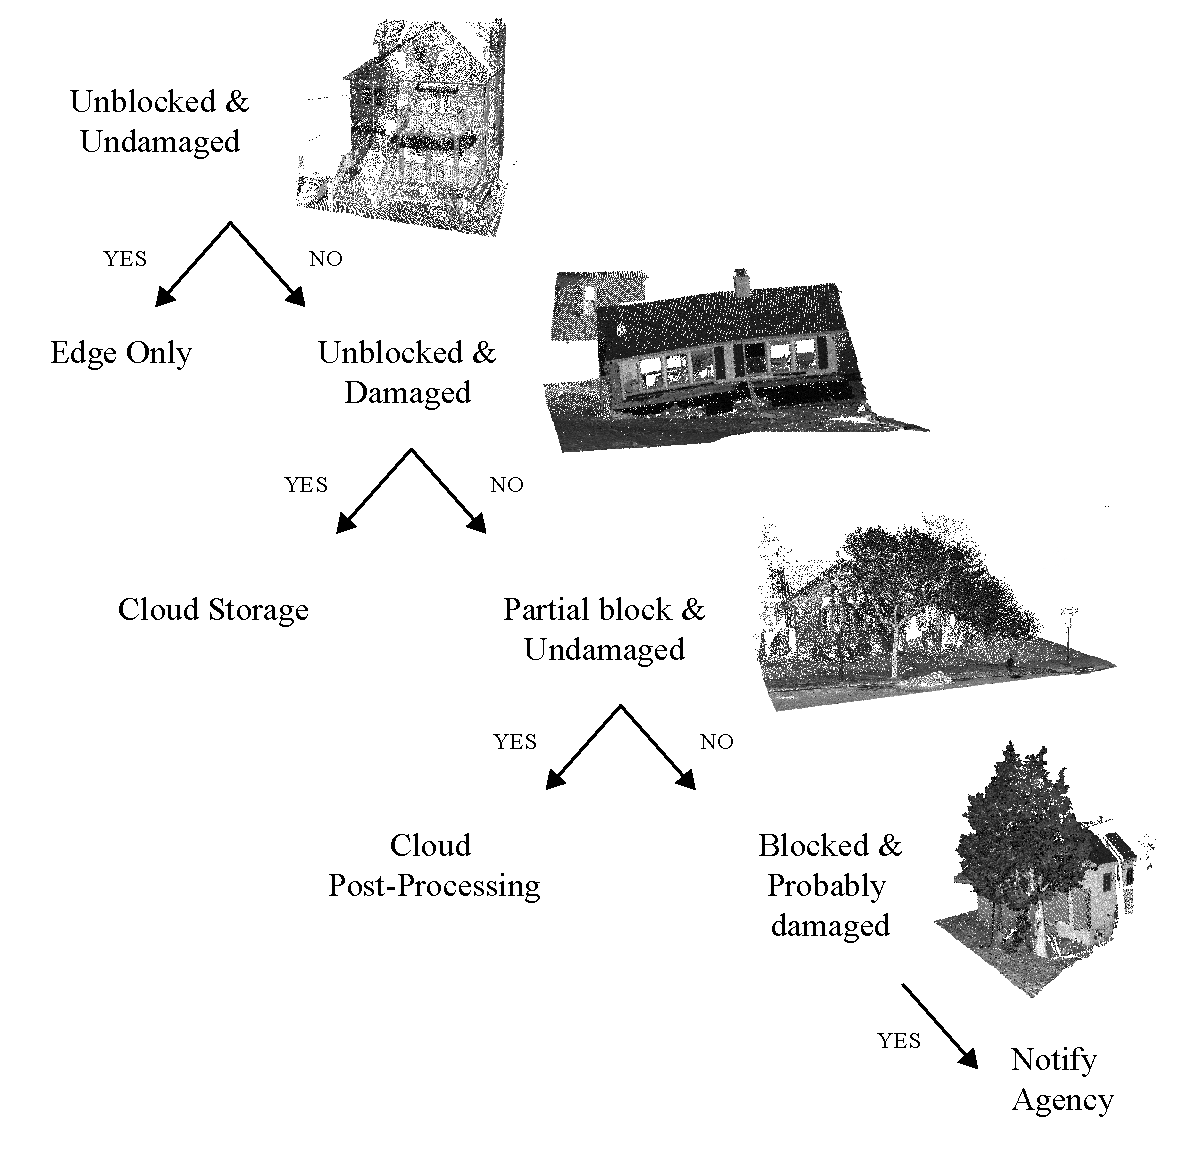
\includegraphics[width=0.5\linewidth]{Figures/diagonal.pdf}
  \caption{Disaster recovery decision stages and its associated reactions based on the LiDAR images.}
  \label{data_uncertainty}
\end{figure}

This workflow presents a content-driven stage where the stream-processing engine needs to perform decisions based on the content of the data that is being processed. Figure \ref{data_uncertainty} depicts all the different content-driven stages that our workflow presents in a decision tree way and its associated reactions. 

The workflow consists of multiple different stages driven by the content of the data (more data content variety means more stages), but only two of them need stream-processing capabilities. The first stage with stream-processing needs is where data gets generated and pre-processed; this stage is performed at the edge of the network so we can quickly and efficiently determine whether the building conditions are safe or not for evacuees to return. Depending on the results from this stage, we trigger the rest of the stages. The second stage, that also needs stream processing, is the change detection application which is executed in the cloud.

\subsubsection{Stage 1: Data generation - Pre-processing Stage}
The following are the actual pre-processing stages that we implemented in Apache Storm to determine the  conditions of the buildings.

\noindent\textbf{Noise Filtering:} flags or removes noise points in the LiDAR data.
\\
\noindent\textbf{Ground Point Classification:} it classifies the LiDAR points into ground object points and non-ground object points.
\\
\noindent\textbf{Classification:} it classifies the point features according to the geometry information. 
\\
\noindent\textbf{Visual inspection:} is designed to provide visual inspection, which allows experts or agencies to access the data and perform visual inspections and help perform more informed decisions.
\\
\noindent\textbf{Content-driven stage:} the last stage on the workflow is a content-driven stage where, depending on the results of the data, we might need to react and trigger further processing to determine if a building is safe or not for evacuees to return. The decision of whether or not data needs post-processing is based on two metrics obtained from the first stage of the pre-processing workflow. The two metrics are: data quality and computation intensity. 
\\
\\
Measurement of data quality: 
\begin{equation}
DQ=\frac{Spacing}{step\_para}\\
\end{equation}
where \textit{Spacing} represents the average edge length (2D) to all neighbor points of the original LiDAR data and \textit{step\_para} represents to the cell size (or the grid size) parameter of the grid-based interpolation.\\
\\
Measurement of computation intensity: 
\begin{equation}
CI=\frac{FileSize}{(X\_lowe - X\_upper) \cdot (Y\_lowe - Y\_upper)}
\end{equation}
\\
\noindent If both the data quality and the computation intensity do not satisfy the specified threshold then further processing is required and the second stage will be performed. 

Since this first stage will be performed at the edge of the network with limited computation capabilities, the user needs to have the ability to specify QoS metrics. In this case the user has the ability to specify a deadline that all the tuples have to meet, as one wants to get the results as fast as possible. 

The following mathematical expressions are the task optimization model proposed for this workflow:
\begin{equation}
\begin{split}
\max \sum x_{ij}
\\
\sum t_{ij} \cdot x_{ij} \leq t_{constraint} , \forall i
\\
x_{ij} \in {0,1}, \forall i,j
\end{split}
\end{equation}

\noindent Where $x_{ij}$ detonates the $j$th tasks at the processing level $i$. $x_{ij} \in {0,1}$ where $x_{ij} = 1$ indicates the execution of the process, while $x_{ij} = 0$ represents not executing the process. $t_{ij}$ denotes the estimated runtime of task $x_{ij}$. $t_{constraint}$ is the total workload budget for all tasks at level $i$.

\subsubsection{Stage 2: Change detection - Post-processing stage}
The following are the actual post-processing stages that we implemented and are triggered based on the content of the data.

\noindent\textbf{Historical data:} the first decision process to determine whether the data that needs further processing has any geo-spatial overlaps with the historical data that is currently stored in the system.

\noindent\textbf{Change detection:} the process that involves comparing changes between LiDAR photographs taken over different time periods that cover the exact same geographic area to understand how a given area has changed between two time periods. 

\noindent\textbf{Content-driven stage:} this stage will notify agencies if the results produced are alarmingly atrocious. 
\\
\\
\noindent To simulate this workflow we used real LiDAR images that were taken right after Hurricane Sandy struck back in 2012 in the NY and Long Island area, with a total of 741 images and 3.7 GB in size, with the biggest image size of 33.8 MB, and the smallest of 1.8 KB. For the historical data in stage 2 we used a bigger data set of pre-Hurricane Sandy. Supporting workflows that generate such large amounts of information at the edge of the network and having to transfer data back and forth between the edge and the core can prevent an effective reaction to an emergency situation and/or target application objectives.

\subsection{Scientific Observatory}

It's a networked ocean research observatory with arrays of instrumented water column moorings and buoys, profilers, gliders, and autonomous underwater vehicles within the different open ocean and coastal regions. OOI infrastructure also includes a cabled array of instrumented seafloor platforms and water column moorings on the Juan de Fuca tectonic plate. This networked system of instruments, moored and mobile platforms, and arrays provide ocean scientists, educators, and the public the means to collect sustained, time-series data sets to enable the examination of complex, interlinked physical, chemical, biological, and geological processes operating throughout the coastal regions and open ocean. OOI implements a geographically distributed, secure, highly available CI that is responsible for data acquisition/collection, data storage and processing, and on-demand delivery of data and data products to scientists and application developers. The use of a well-defined API based on standard protocols enables other systems to interface and interact with OOI CI programmatically. The scientific observatory use case has a similar problem to the disaster recovery use case where the data is to big to send to the cloud in order to offer real-time data delivery.

\subsection{Video Analytics} 

The last use case is the use of video analytics~\cite{8358733} for safety and security. In video analytics, a single video camera can produce about 25-30 frames/second. In HD and FHD cameras an 8-bit uncompressed RGB frame amounts to about 553 Mbps and 1.24 Gbps for a one minute video, respectively. With the advent of 4k and 3D video cameras, this size is likely to grow exponentially. Developers and engineers are facing the challenge of providing on-time analytics of video data to support public safety and security from video cameras. Cloud computing is not efficient enough to support prompt analytics of such video data~\cite{7488250}. Video Analytics based on edge computing is the only feasible approach to cater to low latency requirement for large-scale video streams~\cite{8057318}.

\subsection{Observe Orient Decide Act Loop}

The \ac{OODA} loop refers to the decision-making cycle of observe, orient, decide, and act, developed by military strategists and the United States Air Force~\cite{OODA}. \ac{OODA} is a decision-making cycle to process data streaming from sensors in real time, becoming an essential design characteristic for IoT applications. 
\begin{figure}[h!]
  \centering
  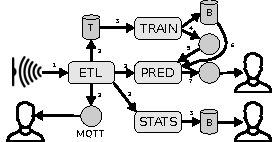
\includegraphics[width=0.8\columnwidth]{Figures/ooda.pdf}
  \caption{RIoTBench IoT high-level logical interactions between different sensors, applications and users.}
  \label{fig:etl}
\end{figure}

Anshu \textit{et al.}~\cite{RIoTBench} offer a suite of IoT applications that follows the closed-loop \ac{OODA} cycle. The applications are based on common IoT patterns for data pre-processing, statistical summarization, and predictive analytics. These are coupled with workloads sourced from real IoT observations. A high-level overview of the logical interaction of the IoT applications is depicted in Figure~\ref{fig:etl}.

\textbf{Extract-Transform-Load (ETL)} consumes data from hundreds of thousands of edge sensors, and pre-processes, cleans, and archives the data. Further, the results are published to an edge broker so that clients interested in real-time monitoring can subscribe to it, while a copy is forked to the cloud for storage, and another to the next dataflow step.

\textbf{Statistical Summarization (STATS)} performs higher order aggregation and plotting operations, and stores the generated plots into the cloud, from where webpages can load the visualization files on browsers. 

\textbf{Model Training (TRAIN)} periodically loads the stored data from ETL step and trains forecasting models that are stored in the cloud, and notifies the message broker of an updated model being available. 

\textbf{The Predictive Analytics (PRED)} subscribe to the message broker and downloads the new models from the cloud, and continuously operates over the pre-processed data stream from ETL to make predictions and classifications that can indicate actions to be taken on the domain. It then notifies the message broker of the predictions, which can independently be subscribed to by a user or device for action. 

The ETL dataflow requires a low-latency cycle in order to achieve real-time monitoring, in addition it also requires some of its operators to be located in the cloud for storing messages and others to be at the edge of the network. This makes the ETL workflow the perfect candidate workflow for testing the operator placement strategy proposed. 
\chapter{Background and Related Work}
\section{Introduction}
Cloud computing was introduced a decade ago with the promise of seemingly infinite computing resources available on demand \cite{Armbrust09abovethe}. This model has proved to be effective for scaling up search engines\cite{7073834}, social networks\cite{6596496}, and content service providers\cite{6915771} to billions of users around the world. However, this centralized model is being challenged by the emergence of a new computing paradigm and associated technologies i.e. Internet of Things (IoT).

The Internet of Things paradigm (IoT) fosters the connection of large numbers of sensors to the network. As the volume of data generated from the devices increases, moving data from the edge of the network to the Cloud might not be feasible due to bandwidth constraints~\cite{8289317}. Furthermore, as low latency and location-aware applications emerge~\cite{7389122}, transfering all the data to the Cloud will not satisfy the low latency or location-aware constraints that the IoT applications expect. In addition, some applications, deal with sensitive and personal data, making it not possible to send the data to the Cloud due to privacy concerns~\cite{7849185}. For example, Toyota estimates that the amount of data flowing between vehicles and servers will reach 10 exabytes per month by 2025~\cite{Toyota}. Another example is commercial jets, which generate 10 TB of data for every 30 minutes of flight, making it impractical to transport all the data from the edge to the Cloud~\cite{ciscoJet}. 

Edge computing has emerged as a potential approach for handling the large quantity of data generated by connected devices. It leverages the ability to execute computations and process data at the edge of the network, closer from the location of data producers. Edge computing leverages smaller servers or single board computers that are widely distributed close to the edge to improve delays. Edge middleware is the essential software stack/architecture that serves as an interface between the Cloud and the IoT devices, supporting data discovery, communication and processing between edge devices and cloud services. %\hl{In this context, edge middleware platforms were created to ease the IoT application development by providing the necessary tools.} 

The realization of edge-based middleware platforms presents several conceptual and technical challenges. We believe that the seamless integration of edge and Cloud systems is one of the main challenges that prevent the efficient utilization of IoT. Without such an integration, developers must explicitly manage the platform as a unified set of resources to orchestrate computations, coordinate devices, and deliver data to users. As a result, there has been a substantial amount of research towards building edge-based middleware, addressing key crosscutting challenges, such as device discovery, scalability, and privacy and security. It is therefore important to understand the current state-of-the-art edge-based middleware and identify the gaps that may exist.

\begin{figure}[hbt!]
    \centering
    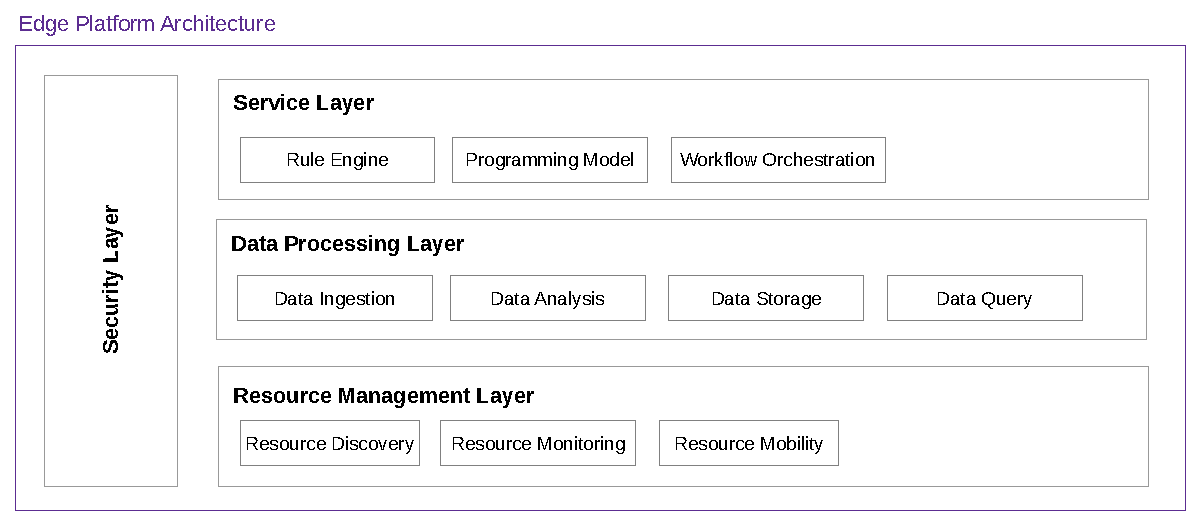
\includegraphics[scale=0.7]{Figures/IoTArchW.pdf}
    \caption{Edge-based middleware reference architecture consisting of four layers, each of them with their respective components.}
    \label{fig:EdgeArch}
\end{figure}

\section{Edge-based Middleware Architecture}\label{sec:arch}

Extensive research and development have been put into creating edge-based middleware systems. There are currently more than 100 edge-based middleware platforms in the market today and the number is continuously growing~\cite{List}. However, not every platform is designed with the same capabilities or architecture. Despite the diversity and large number of edge-based middleware systems, two common architectures emerge:

The majority of IoT platform's architecture follows the Cloud-centric approach. They are built on the premise that ingestion, management, and processing of IoT data can be done in the Cloud, without any edge computing capabilities. Some examples are: Particle Cloud~\cite{Particle}, Salesforce IoT Cloud~\cite{Salesforce_IoT_Cloud} and If This Then That~\cite{IFTTT}.

The other approach is the end-to-end architecture or edge-based middleware architecture built on the premise that edge-processing can save huge costs to clients. %An Internet of Things (IoT) gateway or middleware is a physical device that serves as the connection point between the Cloud and the edge sensors. The gateway or edge middlewares are, usually deployed on single board computers (e.g., Raspberry Pi's), minicomputers, or smart devices (e.g., smartphones, TVs, or refrigerators) to provide management, connectivity, and data pre-processing for sensors.

In this survey, we focus on the end-to-end or edge-based middleware architecture, since the Cloud-centric approach will not be able to satisfy the requirement of the IoT applications presented in section~\ref{sec:usecases}. In order to compare and contrast all the existing state-of-the-art edge-based middlewares, we carefully studied the requirements and limitations of the IoT applications and came up with a four-layer edge-based middleware framework that satisfies all the requirements and limitations of the IoT applications, and each of the middlewares should consist. Figure~\ref{fig:EdgeArch} presents the layers and components that need to be included in an edge-computing solution. The edge-based middleware architecture is composed of four separate layers: resource management, data processing, service , and security.

\begin{table}[hbt!]
\caption{Design goals of the resource management layer components of the cited papers in this survey.}
\label{tab:resource}
\resizebox{\textwidth}{!}{%
\begin{tabular}{c|c|c|c|c|c|c|}
\cline{2-7}
                                          & \multicolumn{2}{c|}{Resource Discovery}               & \multicolumn{2}{c|}{Resource Monitoring}              & \multicolumn{2}{c|}{Resource Mobility}                \\ \hline
\multicolumn{1}{|c|}{Paper}               & Distributed               & \begin{tabular}[c]{@{}c@{}}Low \\Overhead\end{tabular}             & Distributed               & \begin{tabular}[c]{@{}c@{}}Low \\ Overhead\end{tabular}              & Distributed               & \begin{tabular}[c]{@{}c@{}}Low \\ Overhead\end{tabular}              \\ \hline
\multicolumn{1}{|c|}{Paganelli et al.~\cite{article}}    & \checkmark & \checkmark &                           &                           &                           &                           \\ \hline
\multicolumn{1}{|c|}{Liu et al.~\cite{6680268}}          & \checkmark &                           &                           &                           &                           &                           \\ \hline
\multicolumn{1}{|c|}{Cirani et al.~\cite{6899579}}       & \checkmark & \checkmark &                           &                           &                           &                           \\ \hline
\multicolumn{1}{|c|}{Jara et al.~\cite{6550579}}         &                           & \checkmark &                           &                           &                           &                           \\ \hline
\multicolumn{1}{|c|}{Zhou et al.~\cite{6664533}}         &                           & \checkmark &                           &                           &                           &                           \\ \hline
\multicolumn{1}{|c|}{Tanganelli et al.~\cite{8086146}}   &                           &                           & \checkmark & \checkmark &                           &                           \\ \hline
\multicolumn{1}{|c|}{M{\"a}enp{\"a}{\"a} et al.~\cite{Maenpaa2012}}      &                           &                           & \checkmark & \checkmark &                           &                           \\ \hline
\multicolumn{1}{|c|}{SEGUE~\cite{SEGUE}}               &                           &                           &                           &                           & \checkmark & \checkmark \\ \hline
\multicolumn{1}{|c|}{Chaufournier et al.~\cite{Chaufournier:2017}} &                           &                           &                           &                           & \checkmark & \checkmark \\ \hline
\multicolumn{1}{|c|}{Farris et al.~\cite{Farris:2017}}        &                           &                           &                           &                           & \checkmark & \checkmark \\ \hline
\end{tabular}
}
\end{table}

\subsection{Resource Management Layer}
The resource management layer is dedicated to the discovery, identification and allocation of available resources. The challenge of the resource management layer is in managing these limited and geo-distributed resources efficiently. The resource management layer consists of the following components: resource discovery, resource monitoring, and resource mobility. Table~\ref{tab:resource} summarizes the design goals of each of the works focused on the resource management layer.

\subsubsection{Design Goals}

The following are the design goals that need to be taken into consideration when developing any of the components of the resource management layer.
\\\\
\textbf{Low Overhead:} The algorithms and protocols of the resource management layer need to offer low runtime overhead when deployed in performance-limited hardware platforms.
\\\\
\textbf{Distributed:} The resource management components also need to be designed in a distributed fashion in order to scale with the number of applications running in the system and with the number of IoT and edge devices.

%\\\\
%\textbf{Dynamic:} The resource management layer should also be capable to make proactive decisions, dynamic deployment, and intelligent decisions based on the understanding of the context of the environments, users and applications requirements.



\subsubsection{Resource Discovery}
The resource discovery component is responsible for efficiently identifying and discovering the geo-distributed IoT sensors. The following are some of the work focused on the resource discovery component. 

Paganelli et al.~\cite{article} present a service for discovering Internet of Things resources. The service uses a peer-to-peer approach along with distributed hash table (DHT) techniques  to support the discovery of distributed resources, the system guarantees scalability, robustness, and maintainability. Paganelli et al. meet both design goals since they use a distributed architecture by the means of a P2P architecture to support the number of growing devices and offers a low-overhead algorithm.

Liu et al.~\cite{6680268} propose a distributed architecture for resource discovery, designed to be used in Machine-to-Machine applications.
The architecture uses an overlay network composed of peer nodes to distribute workload,and eliminating the single point of failure. Liu et al. resource discovery mechanism only meet the distributed goal since the system is build using a peer-to-peer architecture to efficiently discover the resources in a decentralized manner. It does not meet the low overhead since it used HTTP to communicate and discover resources~\cite{8088251}. The reason being that HTTP runs on TCP, therefore it incurs all TCP connection overheads for connection establishment and closing~\cite{8088251}.

%The architecture is designed to support heterogeneous devices in resource description registration and discovery of resource value. It achieves interoperability among heterogeneous devices in disparate networks and enables resource access from the Internet. In the DRD, a resource registration component is designed for storing resource descriptions; a resource discovery component is designed to retrieve resource values on behalf of clients after getting address information by looking up resource descriptions. 


Cirani et al.~\cite{6899579} also present a Peer-to-Peer architecture for service and resource discovery that can be applied for the Internet of Things applications. Cirani et al. resource discovery mechanism satisfies both goals since it used a distributed P2P architecture for discovering resources and it used CoAP a lightweight messaging system that uses UDP~\cite{8088251} for keeping track of all the resources.

%Utilization of P2P technologies enables deployment of distributed and large scale infrastructure for SD. IoT gateway acts as a backbone of the SD architecture. The gateway keeps track of anything joining or leaving its network and updates the list maintained at its CoAP server. 

Jara et al.~\cite{6550579} presents a centralized mechanism for discovering devices based on context and location. Jara et al. only satisfy the low overhead goal of the resource discovery mechanism since it uses a centralized architecture for discovering devices. It is well-known that centralized architectures have a single point-of-failure and present some scalability concerns when the number of IoT devices grows~\cite{6680268}. 

%An infrastructure called 'digcovery' used for maximizing efficiency and sustainability of deployments offers the framework to allow users to register/include their own sensors into a common infrastructure, and access/discover the available resources through a mobile phone.

Zhou et al.~\cite{6664533} presents a service discovery algorithm and architecture designed for the Internet of Things. The work focuses on the context and location aware discovery. They first present an architecture called "Digcovery" to support the large number of IoT devices. And finally they present a search engine to offer query, look-up and filtering support. Zhou et al. only satisfy the low-overhead goal since the resource discovery mechanism claims that the algorithm has good scalability, and it can be applied to different fields. Only the domain ontology needs to be replaced.

\subsubsection{Resource Monitoring}
The resource monitoring component is responsible for controlling and managing hardware and software infrastructures. It also provides information and performance indicators for both platforms and applications to assist in the decision of allocating the resources. In addition, it monitors the state of the resources in the event of failure. The following are some of the work focused only on the resource monitoring component.

Tanganelli et al.~\cite{8086146} propose an edge-centric architecture that uses the CoRE Resource Directory interface and the CoAP protocol to enable resource monitoring and discovery for IoT applications. This approach is able to satisfy both design goals since it is distributed, in the means of a P2P network, and achieves low overhead since they run their experiments on emulated embedded devices and achieve millisecond latencies.

M{\"a}enp{\"a}{\"a} et al.~\cite{Maenpaa2012} propose an architecture that focuses on the resource discovery and monitoring of wide area sensors and actuators. The architecture enables a federation of geographically distributed Wireless Sensor Networks (WSNs)  using a peer-to-peer network. This approach satisfies both design goals.

\subsubsection{Resource Mobility}
The resource mobility component is responsible for moving computations between edge nodes in order to achieve the requirements of the IoT applications. The following are some of the work focused only on the resource mobility component.

SEGUE~\cite{SEGUE} is a migration system, that achieves optimal migration decisions by using the Markov Decision Process (MDP) to perform migration decisions. SEGUE meets all the design goals since it was carefully evaluated to showcase the real-time performance, scalability, and dynamicity by using real mobility trace of 320 taxis in Rome. 

Chaufournier et al.~\cite{Chaufournier:2017} relies on multi-path TCP, an effort to use multiple paths to maximize resource usage and increase redundancy. This techniques aims at improving the migration time of virtual machines. Chaufournier et al. resource mobility approach also achieves all the goals since it proposed the uses of multi-path TCP and claims that increases the migration throughput by 6x and reduces the time by 50\% in some cases.

Farris et al.~\cite{Farris:2017},presents two Integer Linear Problem optimization schemes, with the pourpus of reducing the quality of service when performing migrations at the edge of the network. Farris et al. resource mobility also meets all the goals since it was designed to cope with the limitation of resource-constrained edge nodes and showcased the scalability in terms of users and the dynamicity of the algorithm.

\begin{table}[h!]
\caption{Design goals of the data processing layer components of the cited papers in this survey.}
\label{tab:processing}
\begin{tabular}{c|c|c|c|c|c|c|c|c|c|c|c|c|}
\cline{2-13}
                                   & \multicolumn{3}{c|}{Data Ingestion}                                 & \multicolumn{3}{c|}{Data Analysis}                                                & \multicolumn{3}{c|}{Data Storage}                                                 & \multicolumn{3}{c|}{Data Query}                                                   \\ \hline
\multicolumn{1}{|c|}{Project}        & \rotatebox[origin=c]{90}{Real-Time} & \rotatebox[origin=c]{90}{Distributed}               & \rotatebox[origin=c]{90}{Scalable}                  & \rotatebox[origin=c]{90}{Real-Time}                 & \rotatebox[origin=c]{90}{Distributed}               & \rotatebox[origin=c]{90}{Scalable}                  & \rotatebox[origin=c]{90}{Real-Time}                 & \rotatebox[origin=c]{90}{Distributed}               & \rotatebox[origin=c]{90}{Scalable}                  & \rotatebox[origin=c]{90}{Real-Time}                 & \rotatebox[origin=c]{90}{Distributed}               & \rotatebox[origin=c]{90}{Scalable}                  \\ \hline
\multicolumn{1}{|c|}{Apache Kafka~\cite{kafka}} &             & \checkmark & \checkmark &                           &                           &                           &                           &                           &                           &                           &                           &                           \\ \hline
\multicolumn{1}{|c|}{Mosquitto~\cite{mosquitto}}    &             & \checkmark & \checkmark &                           &                           &                           &                           &                           &                           &                           &                           &                           \\ \hline
\multicolumn{1}{|c|}{RabbitMQ~\cite{RabbitMQ}}     &             & \checkmark &                           &                           &                           &                           &                           &                           &                           &                           &                           &                           \\ \hline
\multicolumn{1}{|c|}{ActiveMQ~\cite{HiveMQ}}     &             & \checkmark &                           &                           &                           &                           &                           &                           &                           &                           &                           &                           \\ \hline
\multicolumn{1}{|c|}{Heron~\cite{heron}}        &             &                           &                           &                           & \checkmark & \checkmark &                           &                           &                           &                           &                           &                           \\ \hline
\multicolumn{1}{|c|}{Storm~\cite{storm}}        &             &                           &                           &                           & \checkmark & \checkmark &                           &                           &                           &                           &                           &                           \\ \hline
\multicolumn{1}{|c|}{Flink~\cite{flink}}        &             &                           &                           &                           & \checkmark & \checkmark &                           &                           &                           &                           &                           &                           \\ \hline
\multicolumn{1}{|c|}{MillWheel~\cite{millwheel}}    &             &                           &                           &                           & \checkmark & \checkmark &                           &                           &                           &                           &                           &                           \\ \hline
\multicolumn{1}{|c|}{Spark~\cite{spark}}        &             &                           &                           &                           & \checkmark & \checkmark &                           &                           &                           &                           &                           &                           \\ \hline
\multicolumn{1}{|c|}{ApacheEdgent~\cite{edgent}} &             &                           &                           & \checkmark & \checkmark & \checkmark &                           &                           &                           &                           &                           &                           \\ \hline
\multicolumn{1}{|c|}{LMC~\cite{8102173}}          &             &                           &                           & \checkmark &                           & \checkmark &                           &                           &                           &                           &                           &                           \\ \hline
\multicolumn{1}{|c|}{DataFlog~\cite{DataFog:2018}}     &             &                           &                           &                           &                           &                           & \checkmark & \checkmark & \checkmark & \checkmark & \checkmark & \checkmark \\ \hline
\multicolumn{1}{|c|}{FogStore~\cite{Gupta:2018, Mayer2017FogStore}}     &             &                           &                           &                           &                           &                           & \checkmark & \checkmark & \checkmark & \checkmark & \checkmark & \checkmark \\ \hline
\multicolumn{1}{|c|}{Moon et. al.~\cite{8190803}} &             &                           &                           &                           &                           &                           &                           &                           &                           &                           & \checkmark & \checkmark \\ \hline
\multicolumn{1}{|c|}{IOTMDB~\cite{6468294}}       &             &                           &                           &                           &                           &                           &                           &                           &                           &                           & \checkmark & \checkmark \\ \hline
\end{tabular}
\end{table}

\subsection{Data Processing Layer}

The data processing layer is in charge of the consolidation of data from multiple producers, along with its processing and delivery.  Current approaches in data processing are known to be data-intensive process. The frequent operations on disk results in the inability to perform real-time data analytics when executed on edge constrained devices.  The data processing layer consists of four components: ingestion, analysis, storage, and query. Table~\ref{tab:processing} summarizes the design goals of each of the works focused on the data processing layer.
\subsubsection{Design Goals}

The following are the design goals that need to be taken into consideration when designing any of the components of the data processing layer.
\\\\
\textbf{Distributed:} The data processing components should support distributed information processing, distributed computing capabilities, distributed storage and query. In order to address the variable number of devices, services, and users at any given point in time.
\\\\
\textbf{Scalable:} The scalable term refers to the ability of the data processing component to handle a growing number of
clients. The data processing components also need to be scalable also to address the needs of a variable number of devices, services, and users. 
\\\\
\textbf{Real-Time:} The real-time term refers to the ability to achieve low processing latency as the number of messages increases. The data processing components need to be able to process data in real-time either in edge constrained devices such as Raspberry Pis or smartphones and the cloud. Since IoT applications are latency sensitive as we described in section~\ref{sec:usecases}. 

\subsubsection{Data Ingestion}

The data ingestion component aggregates data from multiple producers and sources in order to enable processing through pipelines. The following works focused solely on the data ingestion component.

Apache Kafka~\cite{kafka} is one of the most popular frameworks available, it is an open-source framework used for building real-time data pipelines and streaming apps. Apache Kafka meets three of the four design goals, the reason Apache Kafka does not offer real-time processing at the edge of the network, because it was not designed to be deployed in constrained devices, as it was demonstrated in this work\cite{8778344}.

Mosquitto~\cite{mosquitto} is a lightweight open-source publish/subscribe messaging broker designed for the Internet of Things. It implements the lightweight MQTT protocol, to transport the messages, making it suitable for low-power devices. Even though Mosquitto was created for the need to achieve real-time message handling, Scalagent published a survey where they stress test the Mosquitto and show that it can succeed at handling 60,000 publishers but it requires high transmission latency and high CPU usage~\cite{mqtt}. For those reasons Mosquitto only satisfies the scalability and distributed and scalable design goals.

RabbitMQ~\cite{RabbitMQ} is also a lightweight publish/subscribe messaging broker, designed to be deployed in the cloud.
Similarly to Mosquitto, RabbitMQ in the scaleagent tests shows that it can only handle 8,000 publishers producing 8,000 messages per second, and is not able to achieve real-time analytics~\cite{mqtt}. In this case RabbitMQ only satisfies the distributed goal since it can only support 8,000 publishers, and as mentioned earlier, current city-scale experimental research facilities envision the deployment of 20,000 to 40,000 sensors~\cite{smartsantander}.

ActiveMQ~\cite{HiveMQ} its an open-source messaging broker, that supports numerous industry-standard protocols. ActiveMQ also suffers from the same problems as RabbitMQ since it has high message transmission latency and cannot handle more than 20.000 publishers~\cite{mqtt}.

\subsubsection{Data Analysis}

Data analysis is the process of analyzing large volumes of data to discover useful information and perform informed decisions. The following are some of the work focused on the data analysis component.

Heron~\cite{heron} is a real-time analytics platform developed by Twitter. It is designed for speedy performance, low latency, isolation, and reliability. Heron meets all the design goals except for the real-time data analytics at the edge because it was designed to be deployed in large clusters at the core of the network.

Apache Storm~\cite{storm} is an open-source distributed real-time stream processing system. Similarly, Storm was also designed to be deployed in the Cloud.

Flink~\cite{flink} is a distributed processing engine for performing stream processing applications over unbounded and bounded data streams. Flink was also designed to be deployed in the Cloud and not for the edge.

MillWheel~\cite{millwheel} is a framework for building low-latency data-processing applications that was designed and build by Google. MillWheel, just like Heron, Storm, and Flink, was designed to be deployed in large clusters in the Cloud.

Spark~\cite{spark} is an open-source distributed general-purpose stream processing and batch processing framework witch allow to perform in-memory analytics. Spark, just like Heron, Storm, and Flink, was designed to be deployed in large clusters in the Cloud.

Apache Edgent~\cite{edgent} is a micro-kernel framework designed to be deployed in small footprint edge devices, enabling local, real-time analytics at the edge of the network. Apache Edgent is a stream processing engine that was designed to be deployed on edge devices, allowing it to achieve all the design goals.

LMC~\cite{8102173} enables cross-platform code execution on constrained IoT devices. LCM meets the real-time and the scalable design goals since it was designed to constrained devices , but it doesn't meet the distributed goal since there is no currently not supported.

\subsubsection{Data Storage}

Due to the ever-increasing deployment of bandwidth-intensive IoT platforms (especially cameras), there is an increasing pressure on the bandwidth to transport data back and forth between the edge and the Cloud. There is a need for a more efficient management and computation of the data at the edge of the network. Building a storage system on an edge computing infrastructure has its own set of particular challenges. The wide geo-distribution and heterogeneous and constrained natures of this infrastructure require data-partitioning and replication policies that are commensurate with the latency requirements of the applications. The following are some of the work focused on the data storage component.

DataFlog~\cite{DataFog:2018} is a distributed indexing mechanism that performs data placement (both among edge nodes, and between the edge and the Cloud) based on spatiotemporal attributes to support efficient queries involving multiple edge nodes. DataFlog is able to achieve all the design goals for the data storage layer since it uses distributed indexing mechanism, it supports efficient queries and it can scale since it uses a P2P network and can be deployed in any environment.

FogStore~\cite{Gupta:2018}~\cite{Mayer2017FogStore} is distributed key-value storage system tailored for the edge of the network. FogStore uses a fog-aware replica placement, and a context-sensitive differential consistency strategies to satisfy the requirements of the Edge and the Fog. FogStore was designed by the same authors of DataFog and it also meets all the design goals, just like DataFlog.

\subsubsection{Data Query}

Similarly to the data storage, once data has been stored it needs to be accessed as well. The following are some of the research work on creating edge query systems. The following are some of the work focused on the data query component.
 
Moon et al.~\cite{8190803} propose a data management and searching system based on blockchain which ensures security. Moon et al. are able to meet all the goals for the data query layer except for the real-time design goal since they are using the blockchain Proof-of-Work consensus algorithm and it is known that the time to perform a computation does not increase linearly as the number of nodes increases.

IOTMDB~\cite{6468294} is an IoT storage solution based on NoSQL (Not Only SQL), to solve the storage and management problems of large volumes of IoT data. IOTMDB is able to satisfy all the design goals except for the real-time, since storing 1,000 records can take up to 2 seconds since other frameworks such as RocksDB can store 1,000 records in less than 60 ms~\cite{8778344}.

\begin{table}[h!]
\caption{Design goals of the service layer components of the cited papers in this survey.}
\label{tab:service}
\resizebox{\textwidth}{!}{%
\begin{tabular}{c|c|c|c|c|c|c|c|}
\cline{2-8}
                                       & \multicolumn{2}{c|}{Rule Engine}                      & \multicolumn{2}{c|}{Programming Model}                & \multicolumn{3}{c|}{Workflow Orchestrator}                                        \\ \hline
\multicolumn{1}{|c|}{Paper}            & Scalable                  & \begin{tabular}[c]{@{}c@{}}Low \\ Overhead\end{tabular}              & Expressive                 & Extensible                  & Dynamic                   & Scalable                  & \begin{tabular}[c]{@{}c@{}}Low \\ Overhead\end{tabular}              \\ \hline
\multicolumn{1}{|c|}{Chui et. al.~\cite{5277977}}     & \checkmark & \checkmark &                           &                           &                           &                           &                           \\ \hline
\multicolumn{1}{|c|}{Lica et. al.~\cite{7314063}}     &        \checkmark                   &                           &                           &                           &                           &                           &                           \\ \hline
\multicolumn{1}{|c|}{Mobile-Fog~\cite{Hong:2013}}       &                           &                           & \checkmark & \checkmark &                           &                           &                           \\ \hline
\multicolumn{1}{|c|}{Rabel~\cite{ravel-riliskis-iotapp15}}            &                           &                           &        \checkmark                   & \checkmark &                           &                           &                           \\ \hline
\multicolumn{1}{|c|}{Fabryq~\cite{Etemadi2014FabryqUP}}           &                           &                           &       \checkmark                     &          \checkmark                  &                           &                           &                           \\ \hline
\multicolumn{1}{|c|}{FogFlow~\cite{8022859}}          &                           &                           & \checkmark & \checkmark &                           &                           &                           \\ \hline
\multicolumn{1}{|c|}{Eidenbenz et al.~\cite{Eidenbenz:2016}} &                           &                           &                           &                           &                           &                           & \checkmark \\ \hline
\multicolumn{1}{|c|}{Taneja et al.~\cite{Taneja:2017}}    &                           &                           &                           &                           &                           & \checkmark & \checkmark \\ \hline
\multicolumn{1}{|c|}{DROPLET~\cite{8457776}}          &                           &                           &                           &                           & \checkmark & \checkmark & \checkmark \\ \hline
\multicolumn{1}{|c|}{Ghosh et al.~\cite{Ghosh:2018}}     &                           &                           &                           &                           & \checkmark &                           &                           \\ \hline
\end{tabular}
}
\end{table}

\subsection{Service Layer}
The service Layer defines an application's set of available operations to the end user. The service layer is composed of three components: rule engine, programming model, and workflow orchestrator. Table~\ref{tab:service} summarizes design goals of each of the works focused on the service layer.

\subsubsection{Design Goals}

The following are the design goals that need to be taken into consideration when creating any of the components of the service layer.
\\\\
\textbf{Low Overhead} The service layer components need to be able to process data in real-time, i.e. providing fast analysis and data queries when deployed in performance-limited hardware platforms.
\\\\
\textbf{Scalable} The service layer components need to offer good scalability, since there is going to be a large number of rules and a large number of operators that need to be placed.
\\\\
\textbf{Dynamic} This design goal only applies to the workflow orchestrator. The workflow ochestrator needs to be able to orchestrate the workflows based on the runtime characteristics of the nodes. 
\\\\
\textbf{Expressive} This design goal only applies to the programming model. The programming model needs to be easy to express ideas, algorithms, tasks in an easy-to-read and succinct way.
\\\\
\textbf{Extensible} This design goal also only applies to the programming model. The programming model needs to flexible enough that if new capabilities are needed, they can be added to the software without major changes to the underlying architecture.

%\textbf{Portability} The service layer components should be able to be deployed in any cloud or edge enviroment. 
%The recent trend of emergence of heterogeneous subsystems in smart home environment often leads to interoperability problem in managing such systems. Interoperability is defined as the ability of two or more entities to exchange information and to use the information that has been exchanged [2]. In smart home environment, interoperability is concerned with message exchange between two or more subsystems and performing interoperation in a federated and satisfactory manner without the need for external intervention. 

\subsubsection{Rule Engine}

The Rule Engine makes it possible to evaluate data, perform decisions and trigger actions. The following are some of the work focused on the rule engine component.

Chui et al.~\cite{5277977} propose a rule-based system designed to support  heterogeneous IoT devices. The rule-based system is based on Event-Condition-Action (ECA) rule mechanism with SOAP technology. Chui et al. rule engine satisfies all the design goals since they use an Event-Condition-Action (ECA) pattern which allows them to scale the system as the number of rules grows and achieve low overhead.

Lica et. al~\cite{7314063} propose a rule-based architecture that addresses the main issues involved in application management in the Internet of Things. Lica et al. approach satisfies the expressive and extensible goals since further developments are necessary to improve the architecture effectiveness before its final implementation is carried out.

\subsubsection{Programming Models}
Due to the high dynamicity of edge resource, heterogeneity of Cloud and edge resources deploying low latency and scalable applications can be tricky. For this reason, there is a need for high-level programming models that simplify the development of IoT applications across the edge and the Cloud. The following are some of the work focused on the programming model component.

Mobile-Fog~\cite{Hong:2013} is a high-level programming model designed for applications that require large number of sensors and actuators and they are latency-sensitive. Mobile-Fog only satisfies both design goals since it uses a high-level API to program the sensors, making it easy to learn.

Ravel~\cite{ravel-riliskis-iotapp15} proposes a programming model to program applications across embedded devices, edge nodes and cloud nodes by  using an extension of the Model-View-Controller architecture. Ravel satisfies both design goals since it uses a high-level API. %Ravel introduces the concept of space, which binds particular models, controllers, and views to a specific device. The networking complexities between devices are hidden by the distributed model that automatically synchronizes whenever possible. 

Fabryq et al.~\cite{Etemadi2014FabryqUP} propose a proxy programming model to find and control sensors and actuators. Fabryq et al. approach also satisfies both design goals since it uses Javascript as the main programming language and also has a high-level API to program the sensors, making it easy to learn.

FogFlow~\cite{8022859} is a programming model that extends the dataflow programming model, allowing developers fast and easy development of edge and fog applications. FogFlow satisfies both design goals since it extends the Cloud dataflow programming model and makes it suitable for the edge environment, making it easy to learn.

\subsubsection{Workflow Orchestrator}

The Workflow Orchestrator consists of defining how to accommodate the application components (i.e., operators) on the available resources of the network topology to optimize one or more performance metrics~\cite{8752924}. The main challenge is to decide how to split the operators between the edge and Cloud in order to minimize the overall completion time. The workflow placement has been proved to be at least NP-Hard~\cite{Benoit:2013}. The following are some of the work focused only on the workflow orchestrator component.

Eidenbenz et al.~\cite{Eidenbenz:2016} present an algorithm for the Series-Parallel-Decomposable Graphs (SPDG). Eidenbenz et al. only satisfy the real-time design goals since its only a theoretical approach. %The algorithm is able to achieve a constant-factor approximation under the assumptions that the number of resources scales at least logarithmically with the number of computational tasks and the computational cost of the tasks dominates the cost of communication. 

Taneja et al.~\cite{Taneja:2017} propose an approach for deploying application across Cloud and edge resources by using a Module Mapping Algorithm. Taneja et al. meet all the design goals except for the dynamicity since the approach doesn't take into consideration network connectivity or failure of nodes.

DROPLET~\cite{8457776} is an algorithm, that partitions tasks across the edge and Cloud resources, while minimizing the total completion time. DROPLET achieves all the design goals since it is able to react and adapt to dynamic network events and is capable of performing real-time decisions and scale polynomially with increasing the number of operators to place. 

Ghosh et al.~\cite{Ghosh:2018} propose a Genetic Algorithm (GA) meta-heuristic for distributing analytics across edge and Cloud resources to support IoT applications. The main goal of the genetic algorithm is to minimize the end-to-end latency. Ghosh et al. only meet one of the design goals since it takes between 1 - 26 seconds for placing 1 - 50 operators, making it not real-time or scalable when the number of operators grows.

\begin{table}[h!]
\begin{adjustwidth}{1.8cm}{3cm}
\caption{Design goals of the security layer components of the cited papers in this survey.}
\label{tab:security}
\begin{tabular}{|c|c|c|}
\hline
Paper            & End-to-End Security       & Data Privacy              \\ \hline
Lu. et al.~\cite{7869305}       &                           & \checkmark \\ \hline
Shi et al.~\cite{shi}       &                           & \checkmark \\ \hline
Behrens et al.~\cite{7899405}    & \checkmark &                           \\ \hline
Mukherjee et al.~\cite{7987191} & \checkmark &                           \\ \hline
Kothmayr et al.~\cite{6424088}  & \checkmark &                           \\ \hline
\end{tabular}
\end{adjustwidth}
\end{table}

\subsection{Security Layer}
The fourth and last layer is the Security Layer, which consists of keeping the data generated by thousands of IoT devices private and secure. The following are some of the work focused on the end-to-end security component. Table~\ref{tab:security} summarizes the work focused on the security layer.

\subsubsection{Data privacy}

Since the IoT produces large volumes of data easily available privacy protection in IoT its a challenge. The following are some of the work focused only on the data privacy component.

Lu et al.~\cite{7869305} present a lightweight privacy-preserving data aggregation scheme designed to be used in constrained devices. The proposed aggregation schema uses the homomorphic Paillier encryption, Chinese Remainder Theorem, and one-way hash chain techniques to aggregate data.

Shi et al.~\cite{shi} propose an algorithm that allows users to upload encrypted data to an untrusted aggregator, and allows the aggregator to decrypt  statistics for each time interval.

\subsubsection{End-to-End Security}

In this section, we analyze the similarities and differences amongst all the currently available edge-based middleware systems that implement one or more of the layers of our edge-based middleware architecture. To do so we use the proposed edge platform architecture and the goals of each of the layers described in the previous section. Tables~\ref{tab:full_system_no_goals},\ref{tab:full_system_1},\ref{tab:full_system_2},\ref{tab:full_system_3} summarize and offer more details on all the edge middleware surveyed systems, including the design goals that each component satisfies.

AWS Greengrass~\cite{greengrass} is a software stack that allows to locally run computations, messaging, data caching, sync, and Machine Learning  capabilities on devices in a secure way. AWS Greengrass consists of all the four layers presented in section~\ref{sec:arch}. The main limitations of AWS Greengrass are the centralized architecture of the resource management layer, the lack of storage and query of the data processing layer, the use of a similar MQTT broker to Mosquitto for data ingestion violating the real-time design goal for the data processing layer, and the lack the workflow orchestration component in the service layer, leaving it to the end-user for the management and provisioning of the workflows.

Azure IoT Edge~\cite{azure} is a collection of services designed to create end-to-end IoT applications on Azure Cloud. This service is meant for analyzing data at the edge of the network, instead of in the Cloud. Azure IoT, similarly to AWS, takes security very seriously, and uses certificate-based authentication as the primary mechanism for authentication for the Azure IoT Edge platform. Azure IoT also implements all four layers proposed in section~\ref{fig:EdgeArch}. Azure IoT only misses two components: the first one is the workflow orchestrator from the service layer and the second one is the data privacy at the security layer. Azure IoT uses a similar MQTT broker to Mosquitto making it not able to achieve real-time analytics.

EAaaS~\cite{8029781} is an analytics service that enables real-time edge analytics in IoT scenarios. The main focus of the EAaaS is the uses of a unified rule-based analytic model to simplify the user's programming efforts. In addition, they put a great amount of attention on making the system as lightweight and scalable as possible. EAaaS implements two of the four layers; it does not implement the resource management layer or the security layer and misses some components on the layers that it implements. The first components missing are from the data processing layer: EAaaS does not allow the storage or query of data at the edge of the network. From the service layer, EAaS does not implement the workflow orchestrator, forcing the end-user to decide where to place computations to achieve optimal performance.

Google Cloud IoT Edge~\cite{google} is a collection of services that allows  users to manage, and consume IoT data from distributed devices at a large scale, and take actions as needed. Google Cloud IoT Edge follows the same path as the AWS Greengrass, implementing all four layers but missing some critical components on some of the layers. Google Cloud IoT Edge does not support the ability to store or query at the edge of the network. In addition, just like all the commercial systems surveyed so far, it also implements a similar broker to Mosquitto, violating the real-time design goal. Google Cloud IoT Edge does not offer the ability to orchestrate application between the edge and the Cloud.

Everyware IoT~\cite{everyware} is a comperical platform that provides an end-to-end IoT platform with propriotory software and hardware solutions. Everyware IoT implements all four layers but misses some critical components in all the layers. Similar to AWS, Azure, and Google, it lacks the query and storage support at the edge of the network and uses a similar Mosquitto broker for the data ingestion. Additionally, Everyware IoT lacks the rule engine of the service layer making it not possible to trigger or react to events that happen at the edge of the network.

Predix~\cite{predix} is General Electric's commercial software platform for the collection and analysis of data from industrial machines. Predix implements all four layers but misses some critical components. Predix does not offer resource monitoring, storage, or query. In addition, it also doesn't offer the ability to orchestrate workflows between the edge and the cloud.

Bosch IoT~\cite{bosch} is a commercial end-to-end IoT platform that consists of multiple Cloud-enabled services and software packages. Bosch IoT implements all four layers but misses some components. Bosch IoT does not offer the rule engine or the workflow orchestrator of the service layer, and just like all other commercial systems it also implements a similar broker to Mosquitto.

Yanzi~\cite{yanzi} is a commercial IoT platform designed to optimize office costs and productivity. Yanzi implements three of the four layers, lacking the resource management layer and some critical components on other layers. In the service layer, Yanzi misses the rule engine and the workflow orchestrator, and in the security layer, it misses the data privacy component.

R-Pulsar~\cite{8014357,8109157} is an academic architecture that lets you run local analytics, messaging, data storage, and data querying capabilities on edge devices. R-Pulsar is the only one that satisfies all four layers with the most design goals. In addition, is the only architecture that has a full memory-mapped pipeline making it truly real-time. Also, it's one of the few that offers a unified architecture between the edge and the core, allowing it to seamlessly program the edge and the core. A limitation that the majority of the software stacks/architectures present is a split platform architecture between the edge and the core, leaving the end user to manage the scalability, replication, and distribution to the end user. For platforms that use a single architecture such as R-Pulsar, the system takes care of it so the user can focus on developing the application. R-Pulsar is also the only one to offer any application objectives, all the other software do not any application objectives.

FogHorn~\cite{fogHorn} is a commercial software platform that enables to run advanced analytics and machine learning applications at the edge of the network. FogHorn implements all four layers but misses some critical components in some of the layers. In the data processing layer it misses the data storage and query components, not allowing the storage or query of data at the edge of the network. In the service layer, it misses the workflow orchestrator making the end user responsible for the management and provisioning of the resources and workflows. In the security layer, it misses the data privacy component.

GeeLytics~\cite{7389116} is an academic platform, which can perform real-time analytics either at the edge edge, or in the Cloud in a dynamic manner. Geelytics was designed to emphasize the service layer, in particular, the workflow orchestration component. Geelytics enables developers to run stream processing applications across the edge and the Cloud, without the need to consider where each task is located. GeeLytics implements two of the four layers, not implementing the security and the resource management layer. In addition, GeeLytics lacks the rule engine in the service layer and makes use of Mosquitto or Apache Kafka as the data ingestion data processing layer making it hard to scale or perform real-time analytics at the edge of the network.

Fogflow~\cite{8022859} is the evolution of GeeLytics, an academic framework that orchestrates workflows over the Cloud and the edge based on various context, including system context. For this second iteration they improved their workflow orchestration mechanism, added the missing rule engine component, and implemented the resource management layer. Some of the drawbacks existing on the previous version still have not been addressed, such as the use of Mosquitto or Kafka as the data ingestion component, limiting the scalability and the performance at the edge of the network.

OpenMTC~\cite{openMTC} is a commercial open-source implementation of an IoT/M2M middleware with the focus on providing a standard-compliant platform. OpenMTC implements three of the four layers, missing the resource management layer. In the data processing layer it does not allow the storage or query of data at the edge of the network, and just like any other commercial approach, it uses a similar MQTT broker for the data ingestion. In addition in the service layer, it misses the workflow orchestration.

SiteWhere~\cite{SiteWhere} is an industrial open-source platform, that uses a multi-tenant microservice-based infrastructure. SiteWhere implements all four layers and only misses very few components on some of the layers. In the service layer, it lacks the workflow orchestration and in the security layer, it lacks data privacy.

SmartThings~\cite{SmartThings} is a commercial IoT platform designed for the smart houses. SmartThings implements three of the four layers missing the resource management layer and lacks some major components in some layers. In the data processing layer lacks the ability to store or query data at the edge of the network. In the service layer, it also lacks the workflow orchestration.

Kaa~\cite{Kaa} is a commercial-grade IoT platform that is fully customizable. Kaa is one of the commercial systems more complete, implementing all four layers and missing very few components in some layers. The main drawback of Kaa is the lack of workflow orchestration between the edge and the Cloud, and the lack of data privacy in the security layer.

Samsung Artik~\cite{Samsung_Artik} is a commercial IoT platform that 
focuses on unifying hardware, software, the cloud and the edge as a single ecosystem. Samsung Artick implements three of the four layers, missing the resource management layer. The main drawback is the lack of two of the key components in the data processing layer: the storage and query components. In addition, like all other commercial systems, Artick uses an MQTT broker similar to Mosquitto for the data ingestion component.

Ayla Network~\cite{Ayla_Networks} is a commercial end-to-end IoT platform that includes a completely managed Cloud service. Ayla implements all the layers except for the resource management layer. In the data processing layer, it lacks the data storage and query and it uses an MQTT broker for the data ingestion layer. In addition, it also lacks the workflow orchestration component.

Altair SmartWorks~\cite{Altair_Smartworks} is a commercial platform designe as a Platform as a Service (PaaS) for Internet of Things projects, to collect data from objects, store it and build applications. Altair SmartWorks consists of three of the four layers, missing the data management layer. In the data processing layer, it lacks the ability to store and query data at the edge of the network. In also does not offer the ability to orchestrate workflows between the edge and the Cloud.

EdgeX~\cite{edgex} is a commercial open-source IoT microservice framework that allows end uses to chose their sensors from a large ecosystem of 3rd party offerings. EdgeX implements all four layers but lacks some of the components in most layers. In the data processing layer, EdgeX does not support the data storage or query. In addition like all other commercial systems, EdgeX uses an MQTT broker for the data ingestion violating the real-time design goal. In the service layer, it lacks the workflow orchestration.

PiCasso~\cite{8071529} is an academic orchestration engine that deploys services based on specifications and resources availability. PiCasso implements all the layers except for the security layer. PiCasso puts a lot of emphasis in the service layer more, in particular, the workflow orchestration component. PiCasso lacks the storage and query components of the data processing layers.

Hua-Jun Hong et al.~\cite{8241101} is an academic fog computing platform that that focuses on the task distribution between the edge and the cloud. Hua-Jun Hong et al. approach implements three of the four layers, missing the security layer. In addition, it misses most of the components in all layers, since the main focus of this platform is to make deployment decisions to maximize the number of satisfied IoT analytics (operator deployment problem). In the data processing layer lacks the ability to store and query data at the edge of the network.

Cloud4IoT~\cite{7830723} is an academic platform that focuses on automatically deploying and orchestrating IoT applications. Cloud4IoT implements all the layers except for the security layer. Cloud4IoT to ease the code interoperability between the edge and the Cloud, to do that relies on commercial software that was designed to be deployed on a large cluster, making it hard to achieve real-time analytics at the edge of the network.

Nebulae~\cite{Nebulae} is a commercial end-to-end IoT platform, which the main focus in interoperability and inter-portability. Nebulae implements three of the four layers missing the resource management layer. In the data processing layer, it lacks the ability to store and query data at the edge of the network. In the service layer, it lacks the rule engine and the workflow orchestrator.

FogGIS~\cite{7894725} is an academic framework for improving throughput and reducing latency for analysis of geospatial data. FogGIS implements all the layers except for the resource management layer. In addition, FogGIS data processing layer relies on a commercial system designed to be deployed on the Cloud not at the edge with constrained devices, making it hard to achieve real-time analytics.

FOG-engine~\cite{7588914} is an academic end-to-end platform for processing real-time analytics of data near where it is generated. FOG-engine implements two layers, not implementing the resource management and security layers, missing some key components on most layers. In the service layer, it lacks the orchestration and management of resources and workflows.

CEFIoT~\cite{8355149} is an academic end-to-end fault-tolerant architecture that reuses Cloud technologies at the edge of the network. CEFIoT implements two of the four layers, missing the resource management and security layers. In the service layer, it lacks the rule engine.

SAVI-IoT~\cite{8114487} is an academic self-managing programmable IoT platform that leverages both Hybrid Virtual Machines (HVV) and container isolation techniques to manage IoT applications. SAVI-IoT, just like CEFIoT, misses the same layers. The main difference is that SAVI-IoT does not offer a rule engine or a workflow orchestration. Another drawbacks of SAVI-IoT uses Kafka as the data ingestion component and Spark for the data analyses layer making them violate the real-time analytics at the edge of the network when deployed on constrained devices.

Foggy~\cite{8027267} is an academic architectural framework and software platform based on open-source technologies. Foggy main focus is the orchestration of application across the edge and the cloud. Foggy implements three of the four layers, missing the resource management layer. One of the main drawbacks of Foggy is the use of containers for orchestrating resources between the federated resource, making it no able to perform real-time analytics at the edge of the network. In addition, it lacks the ability to support storage and query at the edge of the network.

ISYMPHONY~\cite{8039055} is an academic orchestration framework designed for scaling real-time and on-demand IoT services. ISYMPHONY implements three of the four layers missing the security layer. ISYMPHONY focuses on the service layer in particular in the workflow orchestration layer. In the data processing layer, it lacks the data storage and query components. In addition, it lacks the rule engine in the service layer.

Macchina.io~\cite{Macchina.io} is a commercial IoT SDK that allows to connect sensors, actuators, Cloud services, mobile devices, and humans. Macchina.io implements three of the four layers, missing the resource management layer. In the service layer, it doesn't offer a rule-based engine or the workflow orchestration. In addition, Macchina.io relies on an MQTT broker similar to Mosquitto for the data ingestion layer.

Clearblade~\cite{Clearblade} is a commercial IoT platform to build scalable, secure enterprise IoT solutions. Clearblade implements three of the four layers, missing the resource management layer, and just like every other system it implements Mosquitto as their data ingestion component.

IBM Watson IoT Platform~\cite{IBM} is a commercial IoT platform that can connect and control IoT sensors, appliances, homes, and industries. The IBM Watson IoT Platform relies on the cloud to distribute and manage the edge analytics. IBM Watson IoT Platform implements all four layers proposed but misses the data storage and data query components of the data processing layer. Just like every other commercial systems surveyed above, it uses Mosquitto as their data ingestion component making it not scalable and real-time.

\begin{table*}[t]
\begin{adjustwidth}{-2cm}{-1cm}
\caption{(Appendix 1) Four Layer and Components for all the commercial and academic edge middleware available.}
\label{tab:full_system_no_goals}
\begin{tabular}{c|c|c|c|c|c|c|c|c|c|c|l|c|}
\cline{2-13}
                                                                                      & \multicolumn{4}{c|}{\begin{tabular}[c]{@{}c@{}}Data Processing \\ Layer\end{tabular}}                                                                    & \multicolumn{3}{c|}{\begin{tabular}[c]{@{}c@{}}Resource Management \\Layer\end{tabular}}                                                                        & \multicolumn{3}{c|}{Service Layer}                                                & \multicolumn{2}{c|}{Security Layer}                         \\ \hline
\multicolumn{1}{|c|}{System}                                                           & \rotatebox[origin=c]{90}{Data Ingestion}            & \rotatebox[origin=c]{90}{Data Analysis}             & \rotatebox[origin=c]{90}{Storage}              & \rotatebox[origin=c]{90}{Data Query}                & \rotatebox[origin=c]{90}{\begin{tabular}[c]{@{}c@{}}Resource \\ Discovery\end{tabular}}        & \rotatebox[origin=c]{90}{\begin{tabular}[c]{@{}c@{}}Resource \\ Monitoring\end{tabular}}       & \rotatebox[origin=c]{90}{\begin{tabular}[c]{@{}c@{}}Resource \\ Mobility\end{tabular}}        & \rotatebox[origin=c]{90}{\begin{tabular}[c]{@{}c@{}}Workflow \\ Orchestrator\end{tabular}}     & \rotatebox[origin=c]{90}{Rule Engine}               & \rotatebox[origin=c]{90}{\begin{tabular}[c]{@{}c@{}}Programming \\ Model\end{tabular}}         & \rotatebox[origin=c]{90}{Data privacy} & \rotatebox[origin=c]{90}{\begin{tabular}[c]{@{}c@{}}End-to-End \\ Security\end{tabular}}       \\ \hline
\multicolumn{1}{|c|}{\begin{tabular}[c]{@{}c@{}}AWS Greengrass~\cite{greengrass}\end{tabular}}       & \checkmark & \checkmark &                           &                           &                           & \checkmark                                     &                           &                           & \checkmark & \checkmark &                           & \checkmark \\ \hline
\multicolumn{1}{|c|}{\begin{tabular}[c]{@{}c@{}}Azure IoT Edge~\cite{azure}\end{tabular}}       & \checkmark & \checkmark & \checkmark & \checkmark &                           & \checkmark                                     &                           &                           & \checkmark & \checkmark &                           & \checkmark \\ \hline
\multicolumn{1}{|c|}{EAaaS~\cite{8029781}}                                                           & \checkmark & \checkmark &                           &                           &                           &                                                               &                           &                           & \checkmark & \checkmark &                           &                           \\ \hline
\multicolumn{1}{|c|}{\begin{tabular}[c]{@{}c@{}}Google \\ Cloud IoT~\cite{google}\end{tabular}}     & \checkmark & \checkmark &                           &                           & \checkmark & \checkmark                                     &                           &                           & \checkmark & \checkmark &                           & \checkmark \\ \hline
\multicolumn{1}{|c|}{\begin{tabular}[c]{@{}c@{}}Everyware IoT~\cite{everyware}\end{tabular}}        & \checkmark & \checkmark &                           &                           & \checkmark & \checkmark                                     &                           &                           &                           & \checkmark &                           & \checkmark \\ \hline
\multicolumn{1}{|c|}{Predix~\cite{predix}}                                                          & \checkmark & \checkmark &                           &                           & \checkmark & \checkmark                                     &                           &                           & \checkmark & \checkmark &                           & \checkmark \\ \hline
\multicolumn{1}{|c|}{Bosch IoT~\cite{bosch}}                                                       & \checkmark & \checkmark & \checkmark &                           & \checkmark & \checkmark                                     &                           &                           &                           & \checkmark &                           & \checkmark \\ \hline
\multicolumn{1}{|c|}{Yanzi et. al.~\cite{yanzi}}                                                   & \checkmark & \checkmark &                           &                           &                           &                                                               &                           &                           &                           & \checkmark &                           &  \checkmark                         \\ \hline
\multicolumn{1}{|c|}{R-Pulsar~\cite{8014357,8109157}}                                                        & \checkmark & \checkmark & \checkmark & \checkmark & \checkmark & \checkmark                                     & \checkmark & \checkmark & \checkmark & \checkmark &                           & \checkmark \\ \hline
\multicolumn{1}{|c|}{FogHorn~\cite{fogHorn}}                                                         & \checkmark & \checkmark &                           &                           &                           & \checkmark                                     &                           &                           & \checkmark & \checkmark &                           & \checkmark \\ \hline
\multicolumn{1}{|c|}{GeeLytics~\cite{7389116}}                                                       & \checkmark & \checkmark &                           &                           &                           &                                                               &                           &                           &                           & \checkmark &                           &                           \\ \hline
\multicolumn{1}{|c|}{Fogflow~\cite{8022859}}                                                         & \checkmark & \checkmark & \checkmark & \checkmark & \checkmark & \checkmark                                     &                           & \checkmark & \checkmark & \checkmark &                           & \checkmark \\ \hline
\multicolumn{1}{|c|}{OpenMTC~\cite{openMTC}}                                                         & \checkmark & \checkmark &                           &                           &                           &                                                               &                           &                           & \checkmark & \checkmark &                           & \checkmark \\ \hline
\multicolumn{1}{|c|}{SiteWhere~\cite{SiteWhere}}                                                       & \checkmark & \checkmark & \checkmark & \checkmark & \checkmark & \checkmark                                     &                           &                           & \checkmark & \checkmark &                           & \checkmark \\ \hline
\multicolumn{1}{|c|}{SmartThings~\cite{SmartThings}}                                                     & \checkmark & \checkmark &                           &                           &                           &                                                               &                           &                           & \checkmark & \checkmark &                           & \checkmark \\ \hline
\multicolumn{1}{|c|}{Kaa~\cite{Kaa}}                                                             & \checkmark & \checkmark & \checkmark & \checkmark & \checkmark & \checkmark                                     & \checkmark &                           & \checkmark & \checkmark &                           & \checkmark \\ \hline
\multicolumn{1}{|c|}{Samsung Artik~\cite{Samsung_Artik}}                                                   & \checkmark & \checkmark &                           &                           &                           &                                                               &                           &                           & \checkmark & \checkmark &                           & \checkmark \\ \hline
\multicolumn{1}{|c|}{Ayla Network~\cite{Ayla_Networks}}                                                    & \checkmark & \checkmark &                           &                           &                           &                                                               &                           &                           & \checkmark & \checkmark &                           & \checkmark \\ \hline
\multicolumn{1}{|c|}{\begin{tabular}[c]{@{}c@{}}Altair \\ SmartWorks~\cite{Altair_Smartworks}\end{tabular}}    & \checkmark & \checkmark &                           &                           &                           &                                                               &                           &                           & \checkmark & \checkmark &                           & \checkmark \\ \hline
\multicolumn{1}{|c|}{EdgeX~\cite{edgex}}                                                           & \checkmark & \checkmark &                           &                           & \checkmark & \checkmark                                     &                           &                           & \checkmark & \checkmark &                           & \checkmark \\ \hline
\multicolumn{1}{|c|}{PiCasso~\cite{8071529}}                                                         & \checkmark & \checkmark &                           &                           & \checkmark & \checkmark                                     &                           & \checkmark &                           & \checkmark &                           &                           \\ \hline
\multicolumn{1}{|c|}{\begin{tabular}[c]{@{}c@{}}Hua-Jun Hong \\ et. al.~\cite{8241101}\end{tabular}} & \checkmark & \checkmark & \checkmark & \checkmark & \checkmark & \checkmark                                     &                           &                           &                           & \checkmark &                           &                           \\ \hline
\multicolumn{1}{|c|}{Cloud4IoT~\cite{7830723}}                                                       & \checkmark & \checkmark &                           &                           & \checkmark &                                                               &                           & \checkmark &                           & \checkmark &                           &                           \\ \hline
\multicolumn{1}{|c|}{Nebulae~\cite{Nebulae}}                                                          & \checkmark & \checkmark &                           &                           &                           &                                                               &                           &                           &                           & \checkmark &                           & \checkmark \\ \hline
\multicolumn{1}{|c|}{FogGIS~\cite{7894725}}                                                          & \checkmark & \checkmark & \checkmark & \checkmark &                           &                                                               &                           &                           &                           & \checkmark &                           &                           \\ \hline
\multicolumn{1}{|c|}{FOG-engine~\cite{7588914}}                                                      & \checkmark & \checkmark & \checkmark & \checkmark &                           &                                                               &                           & \checkmark &                           & \checkmark &                           &                           \\ \hline
\multicolumn{1}{|c|}{CEFIoT~\cite{8355149}}                                                          & \checkmark & \checkmark & \checkmark & \checkmark &                           &                                                               &                           & \checkmark &                           & \checkmark &                           &                           \\ \hline
\multicolumn{1}{|c|}{SAVI-IoT~\cite{8114487}}                                                        & \checkmark & \checkmark & \checkmark & \checkmark &                           &                                                               &                           &                           &                           & \checkmark &                           &                           \\ \hline
\multicolumn{1}{|c|}{Foggy~\cite{8027267}}                                                           & \checkmark & \checkmark &                           &                           &                           &                                                               &                           & \checkmark &                           & \checkmark & \checkmark & \checkmark \\ \hline
\multicolumn{1}{|c|}{ISYMPHONY~\cite{8039055}}                                                       & \checkmark & \checkmark &                           &                           &                           &                                                               &                           & \checkmark &                           & \checkmark &                           &                           \\ \hline
\multicolumn{1}{|c|}{Macchina.io~\cite{Macchina.io}}                                                     & \checkmark & \checkmark & \checkmark & \checkmark &                           &                                                               &                           &                           &                           & \checkmark &                           & \checkmark \\ \hline
\multicolumn{1}{|c|}{Clearblade~\cite{Clearblade}}                                                      & \checkmark & \checkmark & \checkmark & \checkmark &                           &                                                               &                           &                           & \checkmark & \checkmark &                           & \checkmark \\ \hline
\multicolumn{1}{|c|}{IBM Watson IoT~\cite{IBM}}                                                  & \checkmark & \checkmark &                           &                           & \checkmark & \checkmark                                     &                           &                           & \checkmark & \checkmark & \multicolumn{1}{c|}{}     & \checkmark \\ \hline
\end{tabular}
\end{adjustwidth}
\end{table*}

\begin{table*}[]
\begin{adjustwidth}{-1.5cm}{-1cm}
\caption{(Appendix 1) Resource management layer and design goals for all the commercial and academic edge middleware available.}
\label{tab:full_system_1}
\begin{tabular}{c|c|c|c|c|c|c|}
\cline{2-7}
                                                                                      & \multicolumn{2}{c|}{Resource Discovery}               & \multicolumn{2}{c|}{Resource Monitoring}              & \multicolumn{2}{c|}{Resource Mobility}                \\ \hline
\multicolumn{1}{|c|}{System}                                                           & Distributed               & \begin{tabular}[c]{@{}c@{}}Low \\ Overhead\end{tabular}              & Distributed               & \begin{tabular}[c]{@{}c@{}}Low \\ Overhead\end{tabular}              & Distributed               & \begin{tabular}[c]{@{}c@{}}Low \\ Overhead\end{tabular}              \\ \hline
\multicolumn{1}{|c|}{\begin{tabular}[c]{@{}c@{}}AWS \\ Greengrass~\cite{greengrass}\end{tabular}}       &                           & \checkmark &                           & \checkmark &                           &                           \\ \hline
\multicolumn{1}{|c|}{\begin{tabular}[c]{@{}c@{}}Azure \\ IoT Edge~\cite{azure}\end{tabular}}       &                           & \checkmark &                           & \checkmark &                           &                           \\ \hline
\multicolumn{1}{|c|}{\begin{tabular}[c]{@{}c@{}}Google \\ Cloud IoT~\cite{google}\end{tabular}}     &                           & \checkmark &                           & \checkmark &                           &                           \\ \hline
\multicolumn{1}{|c|}{R-Pulsar~\cite{8014357,8109157}}                                                        & \checkmark & \checkmark & \checkmark & \checkmark & \checkmark & \checkmark \\ \hline
\multicolumn{1}{|c|}{Fogflow~\cite{8022859}}                                                         &                           & \checkmark & \checkmark & \checkmark &                           &                           \\ \hline
\multicolumn{1}{|c|}{SiteWhere~\cite{SiteWhere}}                                                       &                           & \checkmark &                           & \checkmark &                           &                           \\ \hline
\multicolumn{1}{|c|}{EdgeX~\cite{edgex}}                                                           &                           & \checkmark &                           & \checkmark &                           &                           \\ \hline
\multicolumn{1}{|c|}{PiCasso~\cite{8071529}}                                                         &                           &                           & \checkmark & \checkmark &                           &                           \\ \hline
\multicolumn{1}{|c|}{\begin{tabular}[c]{@{}c@{}}Hua-Jun Hong \\ et. al.~\cite{8241101}\end{tabular}} &                           &                           &                           & \checkmark &                           &                           \\ \hline
\multicolumn{1}{|c|}{Cloud4IoT~\cite{7830723}}                                                       & \checkmark &                           & \checkmark &                           &                           &                           \\ \hline
\multicolumn{1}{|c|}{CEFIoT~\cite{8355149}}                                                          &                           &                           &                           & \checkmark &                           &                           \\ \hline
\multicolumn{1}{|c|}{Foggy~\cite{8027267}}                                                           &                           &                           &                           & \checkmark &                           &                           \\ \hline
\multicolumn{1}{|c|}{ISYMPHONY~\cite{8039055}}                                                       &                           &                           &                           & \checkmark &                           &                           \\ \hline
\end{tabular}
\end{adjustwidth}
\end{table*}

\begin{table*}[]
\begin{adjustwidth}{-1cm}{-1cm}
\caption{(Appendix 1) Data processing layer and design goals for all the commercial and academic edge middleware available.}
\label{tab:full_system_2}
\begin{tabular}{|c|c|c|c|c|c|c|c|c|c|c|c|c|}
\hline
                                                                   & \multicolumn{3}{c|}{Data Ingestion}                                               & \multicolumn{3}{c|}{Data Analysis}                                                & \multicolumn{3}{c|}{Data Storage}                                                 & \multicolumn{3}{c|}{Data Query}                                                   \\ \hline
System                                                              & \rotatebox[origin=c]{90}{Real-Time}                 & \rotatebox[origin=c]{90}{Distributed}               & \rotatebox[origin=c]{90}{Scalable}                  & \rotatebox[origin=c]{90}{Real-Time}                 & \rotatebox[origin=c]{90}{Distributed}               & \rotatebox[origin=c]{90}{Scalable}                  & \rotatebox[origin=c]{90}{Real-Time}                 & \rotatebox[origin=c]{90}{Distributed}               & \rotatebox[origin=c]{90}{Scalable}                  & \rotatebox[origin=c]{90}{Real-Time}                 & \rotatebox[origin=c]{90}{Distributed}               & \rotatebox[origin=c]{90}{Scalable}                  \\ \hline
\begin{tabular}[c]{@{}c@{}}AWS \\ Greengrass~\cite{greengrass}\end{tabular}          &                           & \checkmark & \checkmark & \checkmark & \checkmark & \checkmark &                           &                           &                           &                           &                           &                           \\ \hline
\begin{tabular}[c]{@{}c@{}}Azure IoT Edge~\cite{azure}\end{tabular}          &                           & \checkmark & \checkmark & \checkmark & \checkmark & \checkmark &                           & \checkmark & \checkmark &                           & \checkmark & \checkmark \\ \hline
EAaaS~\cite{8029781}                                                             & \checkmark & \checkmark & \checkmark & \checkmark & \checkmark & \checkmark &                           &                           &                           &                           &                           &                           \\ \hline
\begin{tabular}[c]{@{}c@{}}Google \\ Cloud IoT~\cite{google}\end{tabular}        &                           & \checkmark & \checkmark &                           & \checkmark & \checkmark &                           &                           &                           &                           &                           &                           \\ \hline
\begin{tabular}[c]{@{}c@{}}Cisco IoT \\ Cloud Connect~\cite{cisco}\end{tabular} &                           & \checkmark & \checkmark & \checkmark & \checkmark & \checkmark &                           &                           &                           &                           &                           &                           \\ \hline
\begin{tabular}[c]{@{}c@{}}Everyware  IoT~\cite{everyware}\end{tabular}           &                           & \checkmark & \checkmark &                           & \checkmark & \checkmark &                           &                           &                           &                           &                           &                           \\ \hline
Predix~\cite{predix}                                                             &                           & \checkmark & \checkmark &                           & \checkmark & \checkmark &                           &                           &                           &                           &                           &                           \\ \hline
Bosch IoT~\cite{bosch}                                                          &                           & \checkmark & \checkmark &                           & \checkmark & \checkmark &                           &                           &                           &                           &                           &                           \\ \hline
Yanzi et. al.~\cite{yanzi}                                                      &                           & \checkmark & \checkmark &                           & \checkmark & \checkmark &                           &                           &                           &                           &                           &                           \\ \hline
R-Pulsar~\cite{8014357,8109157}                                                           & \checkmark & \checkmark & \checkmark &                           &                           &                           & \checkmark & \checkmark & \checkmark & \checkmark & \checkmark & \checkmark \\ \hline
FogHorn~\cite{fogHorn}                                                            &                           & \checkmark & \checkmark &                           & \checkmark & \checkmark &                           &                           &                           &                           &                           &                           \\ \hline
GeeLytics~\cite{7389116}                                                          &                           & \checkmark & \checkmark &                           & \checkmark & \checkmark & \checkmark & \checkmark & \checkmark &                           & \checkmark & \checkmark \\ \hline
Fogflow~\cite{8022859}                                                            &                           & \checkmark & \checkmark &                           & \checkmark & \checkmark & \checkmark & \checkmark & \checkmark &                           & \checkmark & \checkmark \\ \hline
OpenMTC~\cite{openMTC}                                                            &                           & \checkmark & \checkmark &                           & \checkmark & \checkmark & \checkmark & \checkmark & \checkmark &                           & \checkmark & \checkmark \\ \hline
SiteWhere~\cite{SiteWhere}                                                          &                           & \checkmark & \checkmark &                           & \checkmark & \checkmark &                           &                           &                           &                           &                           &                           \\ \hline
SmartThings~\cite{SmartThings}                                                        &                           & \checkmark & \checkmark &                           & \checkmark & \checkmark &                           &                           &                           &                           &                           &                           \\ \hline
Kaa~\cite{Kaa}                                                                & \checkmark & \checkmark & \checkmark & \checkmark & \checkmark & \checkmark & \checkmark & \checkmark & \checkmark & \checkmark & \checkmark & \checkmark \\ \hline
\begin{tabular}[c]{@{}c@{}}Samsung Artik\end{tabular}           &                           & \checkmark & \checkmark &                           & \checkmark & \checkmark &                           &                           &                           &                           &                           &                           \\ \hline
Ayla Network~\cite{Ayla_Networks}                                                       &                           & \checkmark & \checkmark &                           & \checkmark & \checkmark &                           &                           &                           &                           &                           &                           \\ \hline
\begin{tabular}[c]{@{}c@{}}Altair \\ SmartWorks~\cite{Altair_Smartworks}\end{tabular}       &                           & \checkmark & \checkmark &                           & \checkmark & \checkmark &                           &                           &                           &                           &                           &                           \\ \hline
EdgeX~\cite{edgex}                                                              &                           & \checkmark & \checkmark &                           & \checkmark & \checkmark &                           &                           &                           &                           &                           &                           \\ \hline
PiCasso~\cite{8071529}                                                            &                           &                           &                           &                           & \checkmark & \checkmark &                           &                           &                           &                           &                           &                           \\ \hline
\begin{tabular}[c]{@{}c@{}}Hua-Jun Hong et. al.~\cite{8241101}\end{tabular}    &                           & \checkmark & \checkmark &                           & \checkmark & \checkmark &                           & \checkmark & \checkmark &                           & \checkmark & \checkmark \\ \hline
Cloud4IoT~\cite{7830723}                                                          &                           & \checkmark & \checkmark &                           & \checkmark & \checkmark &                           & \checkmark & \checkmark &                           &                           &                           \\ \hline
Nebulae~\cite{Nebulae}                                                            &                           & \checkmark & \checkmark &                           & \checkmark & \checkmark &                           &                           &                           &                           &                           &                           \\ \hline
FogGIS~\cite{7894725}                                                             &                           & \checkmark & \checkmark &                           & \checkmark & \checkmark &                           & \checkmark & \checkmark &                           & \checkmark & \checkmark \\ \hline
FOG-engine~\cite{7588914}                                                         &                           & \checkmark & \checkmark &                           & \checkmark & \checkmark &                           &                           &                           &                           &                           &                           \\ \hline
CEFIoT~\cite{8355149}                                                             &                           & \checkmark & \checkmark &                           & \checkmark & \checkmark &                           &                           &                           &                           &                           &                           \\ \hline
SAVI-IoT~\cite{8114487}                                                           &                           & \checkmark & \checkmark &                           & \checkmark & \checkmark &                           &                           &                           &                           &                           &                           \\ \hline
Foggy~\cite{8027267}                                                              &                           & \checkmark & \checkmark &                           & \checkmark & \checkmark &                           &                           &                           &                           &                           &                           \\ \hline
ISYMPHONY~\cite{8039055}                                                          &                           & \checkmark & \checkmark &                           & \checkmark & \checkmark &                           &                           &                           &                           &                           &                           \\ \hline
Macchina.io~\cite{Macchina.io}                                                        &                           & \checkmark & \checkmark &                           & \checkmark & \checkmark &                           & \checkmark & \checkmark &                           & \checkmark & \checkmark \\ \hline
Clearblade~\cite{Clearblade}                                                         &                           & \checkmark & \checkmark &                           & \checkmark & \checkmark &                           &                           &                           &                           &                           &                           \\ \hline
\begin{tabular}[c]{@{}c@{}}IBM Watson IoT~\cite{IBM}\end{tabular} &                           & \checkmark & \checkmark & \checkmark & \checkmark & \checkmark &                           &                           &                           &                           &                           &                           \\ \hline
\end{tabular}
\end{adjustwidth}
\end{table*}


\begin{table*}[]
\begin{adjustwidth}{-2cm}{-1cm}
\caption{(Appendix 1) Service layer and design goals for all the commercial and academic edge middleware available.}
\label{tab:full_system_3}
\begin{tabular}{c|c|c|c|c|c|c|c|}
\cline{2-8}
                                                                                         & \multicolumn{2}{c|}{Rule Engine}                      & \multicolumn{2}{c|}{Programming Model}                & \multicolumn{3}{c|}{Workflow Orchestrator}                                        \\ \hline
\multicolumn{1}{|c|}{System}                                                              & Scalable                  & \begin{tabular}[c]{@{}c@{}}Low \\ Overhead\end{tabular}              & Expressive                & Extensible                & Dynamic                   & Scalable                  & \begin{tabular}[c]{@{}c@{}}Low \\ Overhead\end{tabular}              \\ \hline
\multicolumn{1}{|c|}{\begin{tabular}[c]{@{}c@{}}AWS \\ Greengrass~\cite{greengrass}\end{tabular}}          & \checkmark & \checkmark & \checkmark & \checkmark &                           &                           &                           \\ \hline
\multicolumn{1}{|c|}{\begin{tabular}[c]{@{}c@{}}Azure \\ IoT Edge~\cite{azure}\end{tabular}}          & \checkmark & \checkmark & \checkmark & \checkmark &                           &                           &                           \\ \hline
\multicolumn{1}{|c|}{EAaaS~\cite{8029781}}                                                              & \checkmark & \checkmark & \checkmark & \checkmark &                           &                           &                           \\ \hline
\multicolumn{1}{|c|}{\begin{tabular}[c]{@{}c@{}}Google \\ Cloud IoT~\cite{google}\end{tabular}}        & \checkmark & \checkmark & \checkmark & \checkmark &                           &                           &                           \\ \hline
\multicolumn{1}{|c|}{\begin{tabular}[c]{@{}c@{}}Cisco IoT \\ Cloud Connect~\cite{cisco}\end{tabular}} &                           &                           & \checkmark & \checkmark &                           &                           &                           \\ \hline
\multicolumn{1}{|c|}{\begin{tabular}[c]{@{}c@{}}Everyware IoT~\cite{everyware}\end{tabular}}           & \checkmark & \checkmark & \checkmark & \checkmark &                           &                           &                           \\ \hline
\multicolumn{1}{|c|}{Predix~\cite{predix}}                                                             & \checkmark & \checkmark & \checkmark & \checkmark &                           &                           &                           \\ \hline
\multicolumn{1}{|c|}{Bosch IoT~\cite{bosch}}                                                          & \checkmark & \checkmark & \checkmark & \checkmark &                           &                           &                           \\ \hline
\multicolumn{1}{|c|}{Yanzi et. al.~\cite{yanzi}}                                                      &                           &                           & \checkmark & \checkmark &                           &                           &                           \\ \hline
\multicolumn{1}{|c|}{R-Pulsar~\cite{8014357,8109157}}                                                           & \checkmark & \checkmark & \checkmark & \checkmark & \checkmark & \checkmark & \checkmark \\ \hline
\multicolumn{1}{|c|}{FogHorn~\cite{fogHorn}}                                                            & \checkmark & \checkmark & \checkmark & \checkmark &                           &                           &                           \\ \hline
\multicolumn{1}{|c|}{GeeLytics~\cite{7389116}}                                                          &                           &                           & \checkmark & \checkmark &                           &                           &                           \\ \hline
\multicolumn{1}{|c|}{Fogflow~\cite{8022859}}                                                            & \checkmark & \checkmark & \checkmark & \checkmark & \checkmark & \checkmark & \checkmark \\ \hline
\multicolumn{1}{|c|}{OpenMTC~\cite{openMTC}}                                                            &                           &                           & \checkmark & \checkmark &                           &                           &                           \\ \hline
\multicolumn{1}{|c|}{SiteWhere~\cite{SiteWhere}}                                                          & \checkmark & \checkmark & \checkmark & \checkmark &                           &                           &                           \\ \hline
\multicolumn{1}{|c|}{SmartThings~\cite{SmartThings}}                                                        & \checkmark & \checkmark & \checkmark & \checkmark &                           &                           &                           \\ \hline
\multicolumn{1}{|c|}{Kaa~\cite{Kaa}}                                                                & \checkmark & \checkmark & \checkmark & \checkmark &                           &                           &                           \\ \hline
\multicolumn{1}{|c|}{\begin{tabular}[c]{@{}c@{}}Samsung \\ Artik~\cite{Samsung_Artik}\end{tabular}}           &                           &                           & \checkmark & \checkmark &                           &                           &                           \\ \hline
\multicolumn{1}{|c|}{Ayla Network~\cite{Ayla_Networks}}                                                       & \checkmark & \checkmark & \checkmark & \checkmark &                           &                           &                           \\ \hline
\multicolumn{1}{|c|}{\begin{tabular}[c]{@{}c@{}}Altair \\ SmartWorks~\cite{Altair_Smartworks}\end{tabular}}       &                           &                           & \checkmark & \checkmark &                           &                           &                           \\ \hline
\multicolumn{1}{|c|}{EdgeX~\cite{edgex}}                                                              & \checkmark & \checkmark & \checkmark & \checkmark &                           &                           &                           \\ \hline
\multicolumn{1}{|c|}{PiCasso~\cite{8071529}}                                                            &                           &                           & \checkmark & \checkmark & \checkmark & \checkmark & \checkmark \\ \hline
\multicolumn{1}{|c|}{\begin{tabular}[c]{@{}c@{}}Hua-Jun Hong \\ et. al.~\cite{8241101}\end{tabular}}    &                           &                           & \checkmark & \checkmark &                           &                           &                           \\ \hline
\multicolumn{1}{|c|}{Cloud4IoT~\cite{7830723}}                                                          &                           &                           & \checkmark & \checkmark & \checkmark & \checkmark & \checkmark \\ \hline
\multicolumn{1}{|c|}{Nebulae~\cite{Nebulae}}                                                            & \checkmark & \checkmark & \checkmark & \checkmark &                           &                           &                           \\ \hline
\multicolumn{1}{|c|}{FogGIS~\cite{7894725}}                                                             &                           &                           & \checkmark & \checkmark &                           &                           &                           \\ \hline
\multicolumn{1}{|c|}{FOG-engine~\cite{7588914}}                                                         & \checkmark & \checkmark & \checkmark & \checkmark & \checkmark & \checkmark & \checkmark \\ \hline
\multicolumn{1}{|c|}{CEFIoT~\cite{8355149}}                                                             &                           &                           & \checkmark & \checkmark &                           & \checkmark &                           \\ \hline
\multicolumn{1}{|c|}{SAVI-IoT~\cite{8114487}}                                                           &                           &                           & \checkmark & \checkmark &                           & \checkmark &                           \\ \hline
\multicolumn{1}{|c|}{Foggy~\cite{8027267}}                                                              &                           &                           & \checkmark & \checkmark & \checkmark &                           & \checkmark \\ \hline
\multicolumn{1}{|c|}{ISYMPHONY~\cite{8039055}}                                                          &                           &                           & \checkmark & \checkmark & \checkmark & \checkmark & \checkmark \\ \hline
\multicolumn{1}{|c|}{Macchina.io~\cite{Macchina.io}}                                                        &                           &                           & \checkmark & \checkmark &                           &                           &                           \\ \hline
\multicolumn{1}{|c|}{Clearblade~\cite{Clearblade}}                                                         & \checkmark & \checkmark & \checkmark & \checkmark &                           &                           &                           \\ \hline
\multicolumn{1}{|c|}{\begin{tabular}[c]{@{}c@{}}IBM Watson IoT~\cite{IBM}\end{tabular}} & \checkmark & \checkmark & \checkmark & \checkmark &                           &                           &                           \\ \hline
\end{tabular}
\end{adjustwidth}
\end{table*}

\chapter{Associative Rendezvous 2.0 (AR)}
\section{Introduction}

In this Chapter, we describe the semantics and mechanisms that our programming abstraction builds upon, which enable developers to decide \textbf{what} and \textbf{where} data are collected and analyzed. 

Publish/subscribe (pub/sub) systems are widely used in IoT applications such as environment monitoring, supply chain tracing, healthcare, and vehicle networks. The Publish Subscribe model enables event-driven architectures and asynchronous parallel processing, while improving performance, reliability and scalability. Pub/sub protocols, however, make some common task in IoT more challenging to achieve, for instance, it is not straightforward to discover potential publishers of a particular type or in a particular location. The lack of publisher and subscriber discovery is a key challenge that has to be overcome to enable the interoperability of different IoT data providers and producers. For those reasons we chose the Associative Rendezvous (AR), a paradigm for content-based decoupled interactions with programmable reactive behaviors.  AR allows highly expressive descriptions . AR differs from the traditional publish/subscribe paradigms in that it does not relay in topics, it relays on well defined combinations of keywords (i.e.keywords, partial keywords, wildcards, ranges) from a semantic information space to defined the properties of the publisher or subscriber.

Rendezvous-based interactions~\cite{AR} provide a mechanism for decoupling senders and receivers. The Rendezvous Point (RP) is the node where rendezvous interactions occur, and it can be an edge node or a cloud node. Senders transmit messages to an RP without knowledge of who or where the receivers are. The associative rendezvous interaction model consists of three elements, messages, associative selection, and reactive behaviors, which are described below. In the following sections we will first describe the semantics and primitives of AR and then we present the adaptation of AR semantics and primitives to fit our model. The R-Pulsar AR approach is an adaptation of existing primitives from Meteor~\cite{meteor2008}.

\section{Associative Rendezvous} 
Associative Rendezvous is a paradigm for content-based decoupled interactions with programmable reactive behaviors. Rendezvous-based interactions~\cite{AR} provide a mechanism for decoupling senders and receivers. The Rendezvous Point (RP) is the node where rendezvous interactions occur, and it can be an edge node or a cloud node. Senders transmit messages to an RP without knowledge of who or where the receivers are. The associative rendezvous interaction model consists of three elements, messages, associative selection, and reactive behaviors, which are described below. The AR interaction model consists of three elements: messages, associative selection, and reactive behaviors, which are described below~\cite{meteor2008}.

\begin{figure}
    \centering
    \begin{subfigure}[t]{0.5\textwidth}
        \centering
        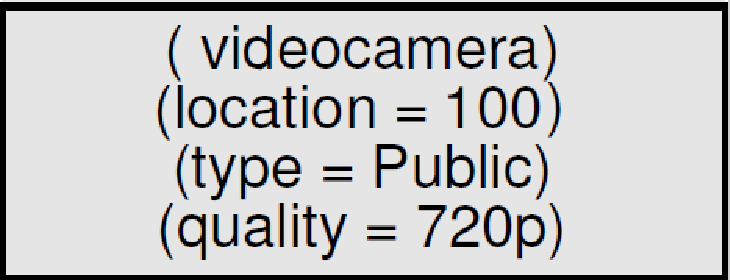
\includegraphics[height=1in]{Figures/data_profile.pdf}
        \caption{}
        \label{fig:data_profile}
    \end{subfigure}%
    ~ 
    \begin{subfigure}[t]{0.5\textwidth}
        \centering
        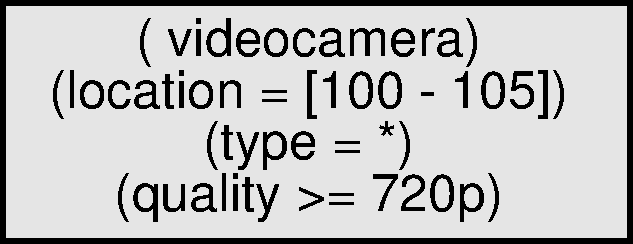
\includegraphics[height=1in]{Figures/interest_profile.pdf}
        \caption{}
        \label{fig:interest_profile}
    \end{subfigure}
    \caption{Sample profiles: (a) producer profile from a video camera sensor; (b) consumer profile interested in video camera sensors}\label{fig:samples_profiles}
\end{figure}



\subsection{AR Message}
An AR message~\cite{meteor2008} is defined as the triplet: (header, action, data). The data field may be empty or may contain the message payload. The header includes a semantic profile in addition to the credentials of the sender, a message context, and the Lifetime of the message. The profile is a set of attributes and/or attribute–value pairs, and defines the set of recipients of the message. The attributes are keywords from the application information space, such as the type of data a sensor produces (temperature or humidity) and/or its location, the type of functionality a service provides and/or its quality of service guarantees, and the capability and/or the cost of a resource, while the values field may be a keyword, partial keyword, wildcard, or range from the same space. At the RP, a profile is classified as a data profile or an interest profile depending on the action field of the message. The data profile corresponds to a message carrying data to be stored in the system. The interest profile corresponds to a query.

\subsection{Associative Selection} 

Profiles are represented using a hierarchical schema that can be efficiently stored and evaluated by the selection engine at runtime. Profile $p$ represents a path in the hierarchical schema, [$e_0$ $\bigtriangleup$ ... $e_k$], where $e_i$ is an element operand and $\bigtriangleup$ can be a parent-child ("/") operator (i.e. at adjacent levels) or an ancestor-descendant ("//") operator (i.e. separated by more than one level). Within a level, the profile defines a propositional expression where $\bigtriangleup$ represents propositional operators, such as $\wedge$ and $\vee$ between elements at the same level. Note that the propositional expression at a level must be evaluated as TRUE for the evaluation to continue to the next level. The elements of the profile can be an attribute, $e_i$ : ($a_i$), or an attribute-value pair $e_i$ : ($a_i$, $v_i$), where $a_i$ is a keyword and $v_i$ may be a keyword, partial keyword, wildcard, or range. The singleton attribute $a_i$ evaluates to true if and only if $p$ contains the simple attribute $a_i$. The attribute-value pair ($a_i$,$u_i$) evaluates to true with respect to a profile $p$, if and only if $p$ contains attribute $a_i$ and the corresponding value $v_i$ satisfies $u_i$. For example, the profile in Figure~\ref{fig:data_profile} will be matched by the profile in Figure~\ref{fig:interest_profile}, since (1) both have matched singleton attribute video camera; (2) for attribute location, 100 - 105, satisfies the range relation; (3) for attribute type, {\it Public} matches the wildcard *; and (4) quality$=$720p satisfies the request quality$>=$720p. 
\\
\begin{table}[h]
\caption{AR Reactive behaviors}
\label{table:OldActions}
\begin{adjustwidth}{-1cm}{-1cm}

\begin{tabular}{ll}
\hline
\textbf{Actions} & \textbf{Semantics}                                                                                                                                                                                                                 \\ \hline
store            & \begin{tabular}[c]{@{}l@{}}Store data profile and data in the system at the RPs\\ Match the data profile with existing interest profiles with 'notify data' action\\ Execute action associated with a matched profile\end{tabular} \\ \hline
retrieve         & \begin{tabular}[c]{@{}l@{}}Match interest profile with existing data profiles\\ Send data associated with the matched profiles to the requester\end{tabular}                                                                       \\ \hline
notify\_data     & Match message profile with existing data/interest profiles.                                                                                                                                                                        \\
notify\_interest & Notify sender if there is at least one match.                                                                                                                                                                                      \\
delete\_data     & Match message profile with existing data/interest profile.                                                                                                                                                                         \\
delete\_interest & \begin{tabular}[c]{@{}l@{}}Notify sender if there is at least one match.\\ Remove all matching data/interest profiles from the system.\end{tabular}                                                                                \\ \hline
\end{tabular}
\end{adjustwidth}
\end{table}

\subsection{Reactive Behaviors} 

The action field of the message defines the reactive behavior of the profile when a match occurs. Every time an RP receives an AR message, the profile is stored and matched against existing profiles. If there is a match, the action of the profile is carried out. Basic reactive behaviors are store, retrieve, notify, and delete. Table~\ref{table:OldActions} summarizes the available actions.

The notify and delete actions are explicitly invoked on a data or an interest profile. The store action stores the data and data profile at the RP. It also causes the message profile to be matched against existing interest profiles with notify data action, and the data to be sent to the data consumers that requested it in case of a positive match.

The retrieve action retrieves data corresponding to each matching data profile. The notify action matches the message profile against existing interest/data profile, and notifies the sender if there is at least one positive match. 

The notify action comes in two flavors: notify data and notify interest. Notify data is used by data consumers, who want to be notified when data matching their interest profile are stored in the system. Notify interest can be used by data producers, who want to be notified when there is interest in the data they produce, so that they can start sending data into the system.

Finally, the delete action deletes all matching interest/data profiles. Note that the actions will only be executed if the message header contains an appropriate credential. Also note that each message is stored at the rendezvous for a period corresponding to the Lifetime defined in its header. In case of multiple matches, the profiles matching are processed in random order.

\section{R-Pulsar Associative Rendezvous}\label{sec:semantics}
R-Pulsar uses a custom implementation of the original AR semantics~\cite{meteor2008}. In our new implementation of the AR model, we modified to elements: the AR Message and the Reactive Behaviors.

The AR message is now defined as a quintuplet instead of the original triplet: (header, action, data, location, and data-processing task). The location and data processing task fields have been added in to the already existing fields. The location field has been added so the AR message can be routed based on the location and the content, where the original version of AR only routes messages based on the content. The location coordinates represent the physical location of the sensors or the physical location of where to deploy data-processing tasks and the tag helps decide where to deploy data-processing tasks, either the edge or the cloud, allowing to pick from multiple cloud or edge geographically distributed resources.

\begin{table}[t]
\caption{R-Pulsar Reactive behaviors}
\label{table:actions}
\begin{adjustwidth}{0cm}{-1cm}
\begin{tabular}{ll}
\hline
\textbf{Actions} & \textbf{Semantics}                                                                                                                                  \\ \hline
store            & Store data in rendezvous point queue.                                                                                                               \\ \hline
profiles         & \begin{tabular}[c]{@{}l@{}}Notify sender all the interest\_profiles stored in that rendezvous\\ point.\end{tabular}                                 \\ \hline
store\_topology  & Store the new topology in the RP.                                                                                                                   \\
start\_topology  & Start the topology in the RP.                                                                                                                       \\
stop\_topology   & Stop the topology.                                                                                                                                  \\
delete\_topology & Delete the topology.                                                                                                                                \\ \hline
notify\_data     & Match message profile with existing data/interest profiles.                                                                                         \\
notify\_interest & Notify sender if there is at least one match.                                                                                                       \\
query\_data      & Allows to perform SQL-like queries on stored data.                                                                                                  \\
delete\_data     & Match message profile with existing data/interest profile.                                                                                          \\
delete\_interest & \begin{tabular}[c]{@{}l@{}}Notify sender if there is at least one match.\\ Remove all matching data/interest profiles from the system.\end{tabular} \\ \hline
\end{tabular}
\end{adjustwidth}
\end{table}

For the reactive behaviors are now classified in two two different classes: resource actions and function actions. Where in the original implementation of AR there where only one type of actions. Table~\ref{table:actions} summarizes the available actions.

Resource actions are designated for discovering, starting, and stopping sensors from transmitting data. Basic resource reactive behaviors currently defined include {\it notify\_interest, notify\_data, query\_data}, and {\it delete}. The {\it notify\_interest} is used by sensors for advertising its data producing capabilities and that they want to be notified when there is someone interested in the data they can produce. The {\it notify\_data} are used by the data-processing tasks that will consume the data produced by sensors. When a {\it notify\_data} profile and a {\it notify\_interest} profile match, Figure~\ref{fig:samples_profiles} sensors are notified to start streaming data to the consumer. The {\it query\_data } action is for performing SQL-like queries on stored data. The {\it delete} action deletes all matching profiles from the system.

Function actions are designated for storing, triggering, and stopping data-processing tasks. Basic function reactive behaviors currently defined include {\it store\_function, start\_function and stop\_function}. The {\it store\_function} action allows users to submit and store user-defined data-processing tasks in the RPs, allowing to share and discover existing data-processing tasks previously uploaded by other users. This avoids the need to rewrite the same function multiple times and facilitates the reproducibility of the experiments. The {\it start\_function} allows users to trigger data-processing tasks on demand. If there is a match between two profiles, the data-processing task is executed. The {\it stop\_function} allows users to stop data-processing tasks that are running. 

\subsection{Illustrative Example}

This section illustrates two operation examples of the R-Pulsar AR model. The first example in Figure~\ref{fig:ARExample} illustrates the exchange of messages for subscribing to sensors in R-Pulsar. The second example in Figure~\ref{fig:AR-Multi} demonstrates the one-to-many interactions using the R-Pulsar associative rendezvous.

\begin{figure}[h]
\centering
\begin{subfigure}[b]{0.8\textwidth}
   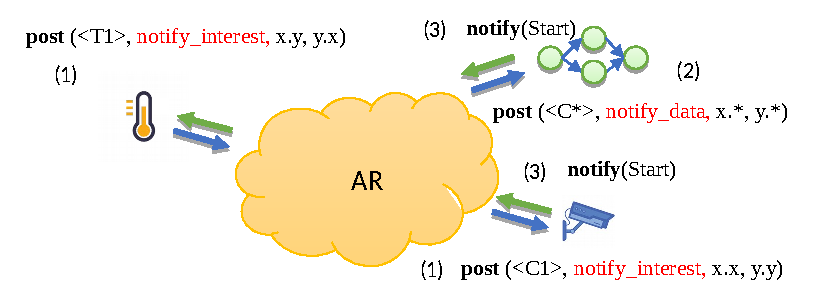
\includegraphics[width=1.1\linewidth]{Figures/AR_Exmple_1.pdf}
   \caption{}
\end{subfigure}
\begin{subfigure}[b]{0.8\textwidth}
   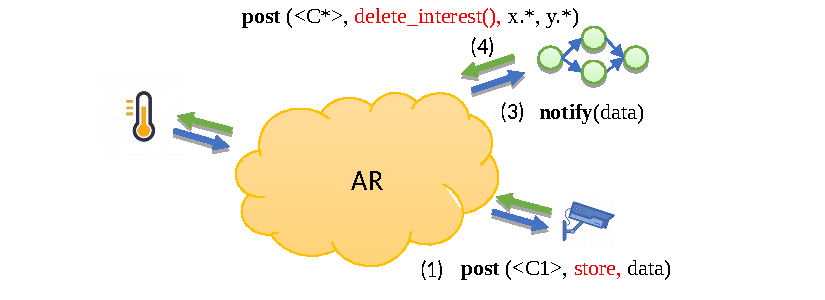
\includegraphics[width=1.1\linewidth]{Figures/AR_Example_2.pdf}
   \caption{}\label{fig:ARExample2} 
\end{subfigure}
\caption{An example illustrating the operation of associative rendezvous.}\label{fig:ARExample} 
\end{figure}

For this example we have two different types of data producers/sensors in this case we have a temperature sensors and a CCTV camera as data producers. In step (1) both sensors perform is to register themselves into the system by advertising the type of data they can produce and where they are located, in the case of the temperature sensor its described by the profile $<T1>$, x.y,y.x and $<C1>$ x.x, y.y for the CCTV camera. By doing that they are requesting to be notified if there are other clients interested in the type of data that they can produce. Both interest profiles are stored in the system, and matched against existing interest profiles. Since there is no interest profiles stored in the system nothing else happens. Both data producers/sensors publishes data in the system only if other clients need it. In step (2) the data consumer/computation is interested in consuming a very specific type of data, in this case it is interested in consuming data that matches the profile $<C*>$ and it is located in x.*,y.*.,  requesting to be notified if there are data stored in the system matching the profile. The interest profile of the computation is stored in the system and matched against the other profiles in the system. Since the notify data profile matches the profile of the CCTV camera, in step (3) a notification message is sent to the CCTV camera that someone is interested in its data and to start pushing the data into the system. In Figure~\ref{fig:ARExample2} step (4) the camera starts publishing data in the system, the data published by the camera matches the data profile specified by the computation,  resulting in step (5) the data being send to the computation for processing. After a few minutes the computation decide that the data the CCTV camera is producing is no longer valuable and decides the unsubscribe from it by sending a delete interest in step (6), pushing a notification to the CCTV camera to sop pushing data to the system.

\begin{figure}[h!]
  \centering
  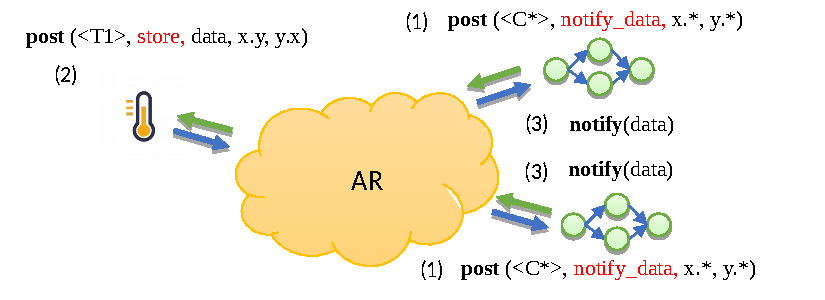
\includegraphics[width=0.8\textwidth]{Figures/AR_Example_Multi.pdf}
  \caption{One-to-many interactions using associative rendezvous.}
  \label{fig:AR-Multi}
\end{figure}

AR can also be used to realize different interaction semantics such as one-to-many, one-to-some and one-to-all. Figure~\ref{fig:AR-Multi} illustrates a one-to-many (e.g. multicast) interaction using AR. The example assumes that the temperature sensor has already been registered in the system with the notify interest profile $<T1>$. In step (1) the two data consumers register in the system requesting to be notified if there are data stored in the system matching the profile. In step (2) the interest profile of the computation is stored in the system and matched against the other profiles in the system. Since the notify data profile matches the profile of the temperature sensor, a notification message is sent to the temperature sensor that someone is interested in its data and to start pushing the data into the system. In step (3) the temperature sensor published data into the system. In step (4) the data published by the sensor matches the notify data profile of the two consumers so both consumers are notified with the data.
\chapter{Enabling Data-driven IoT Applications}
%\section{Framework}
In this chapter, we present our concepts in which R-Pulsar have been build upon. R-Pulsar is a software stack that extends cloud capabilities to edge devices, allowing to collect and analyze data closer to the source of information and react autonomously to local events. R-Pulsar consists of four layers: (1) the infrastructure layer, (2) the federation layer, (3) the streaming layer, and (4) the application layer. Each of the layers consists of multiple components.

\begin{figure}[!h]
  \centering
  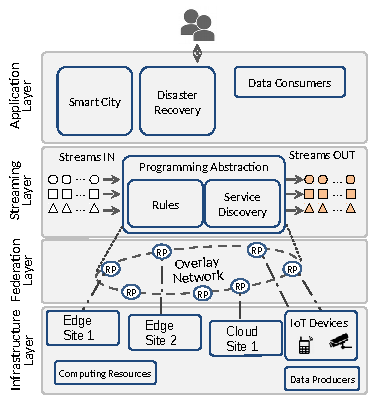
\includegraphics[width=0.7\columnwidth]{Figures/R-PulsarArch.pdf}
  \caption{Schematic overview of the R-Pulsar Architecture}\label{fig:R-PulsarArch}
\end{figure}

\section{Infrastructure Layer}
The infrastructure layer is composed of data producers and computational resources. The data producers are the various streaming sources that can generate data, including IoT devices (e.g., cameras, smart watch, and smart infrastructures, etc). The computational resources are a group of computers responsible for running the applications the user deploys. The resources are heterogeneous and distributed through the infrastructure, from the core to the edge of the network. 

R-Pulsar uses a distributed architecture by the means of an overlay network, where each resource/node in the overlay network is called a Rendezvous Point (RP). RPs can be part of a public or private gateways located at the edge of the network or public or private server located in the cloud. 

\section{Federation Layer}
The federation layer is responsible for orchestrating the geographically distributed resources composing the infrastructure. This layer is built using two main components: the location aware overlay component and the content based routing component.

\subsubsection{Location-aware Overlay Network Component}

\begin{figure}[!h]
  \centering
  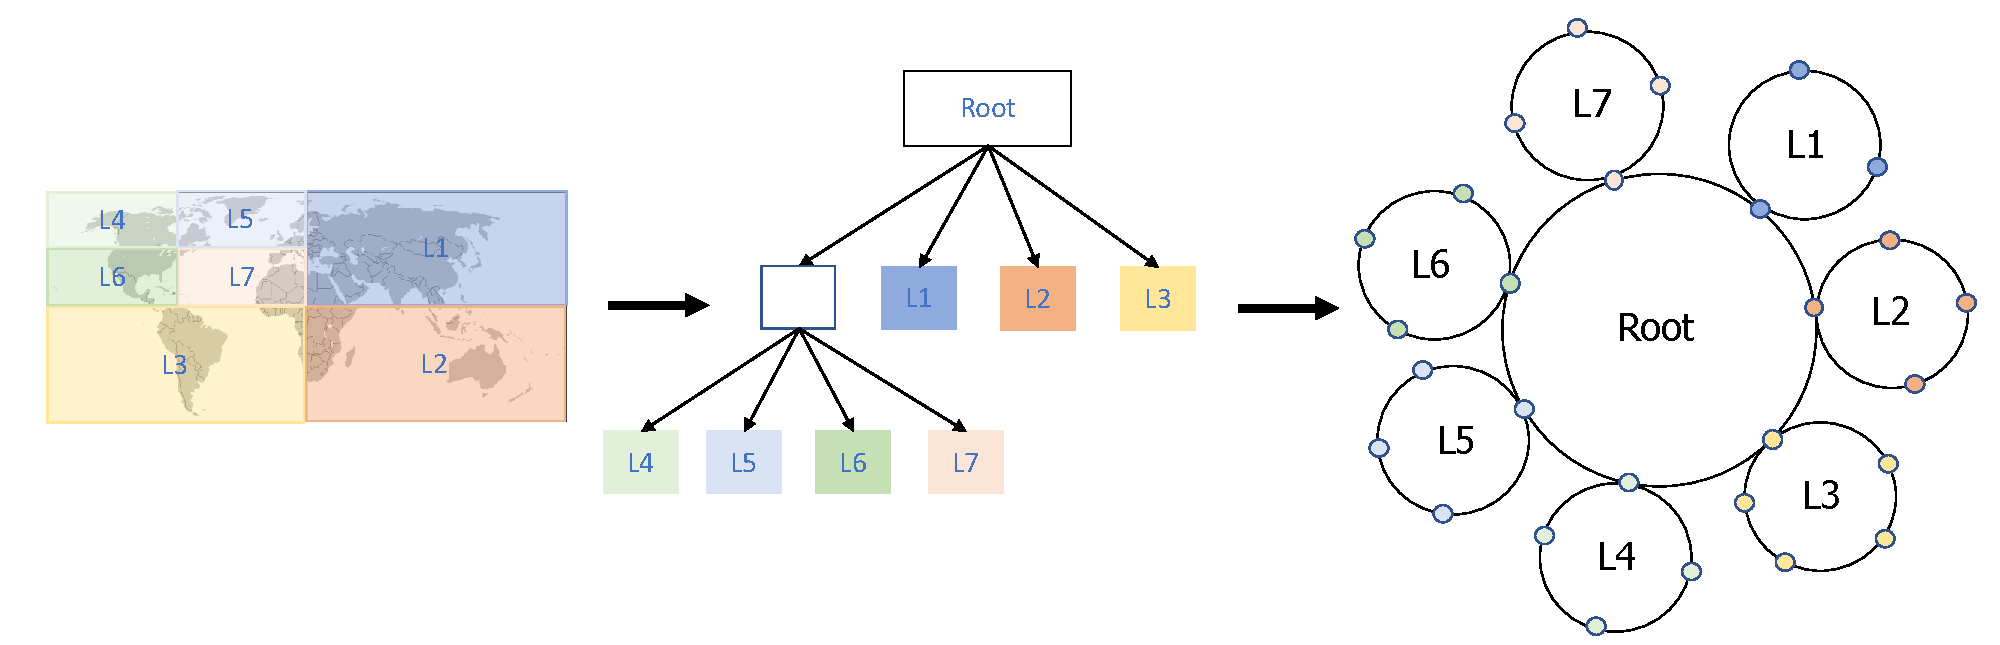
\includegraphics[width=1\columnwidth]{Figures/quadtree.pdf}
  \caption{}\label{fig:quadT}
\end{figure}

IoT data comes with temporal and spatial information, which is directly associated with their business value in a given context. Hence, IoT applications must process data in a timely fashion and from proper locations. In order to process data from the right location R-Pulsar uses a location-aware overlay network in conjunction with a point quadtree to logically groups of RPs that are physically close together. A point quadtree is a tree data structure in which each internal node has exactly four children. Each node represents a 2D bounded box covering a specific part of the space to index, using a root node to cover the entire area.

%The RPs are grouped based on the geographical location to guarantee that data gets processed with minimal latencies.

The R-Pulsar overlay network is an n-dimensional self-organizing structured overlay composed of RP nodes. Peers in the overlay can join or leave the network at any time. Every node in the overlay is assigned a unique identifier that consists of a 160bit unique identifier. Each node stores the keys that maps to the segment of the curve between itself and its predecessor node.

During the initialization of the overlay network, the RP attempts to discover an already existing RP in the system and construct its routing table. The joining RP sends a discovery message to the group. If the message remains unanswered after a duration (in the order of seconds), the RP assumes that it is the first in the system and it becomes the master RP, creating a single overlay network (Peer-to-Peer network). Every time any other RP joins the overlay network and the master RP responds to the discovery message, the  RP is added to the system by using the location of the RP and determining which quadrant the RP occupies. Once the initial P2P network has a sufficient number of RPs to guarantee that in case of multiple failures the P2P network will not disappear, the quadtree subdivides the overlay network into four additional P2P rings, plus an extra ring that will allow all the master RPs of each ring to communicate. Each RP master keeps a copy of the quadtree, so in the case of an RP failure the overlay network structure will never be lost. In the case of a master RPs failure, a master RP election is performed using the Hirschberg and Sinclair algorithm~\cite{Hirschberg}. Figure~\ref{fig:quadT} is a graphical representation of the quadtree and the logical organization of the P2P network.

In order to route a message the first strep is perform a quadtree query to decide in which of the P2P rings needs to be routed to. The locations in the AR message is used to perform a lookup in the tree and find the P2P ring closes to the given location. 

\subsubsection{Content-based Routing Component}\label{sec:frameworkc}

\begin{figure}
\centering
\begin{subfigure}[b]{0.9\textwidth}
   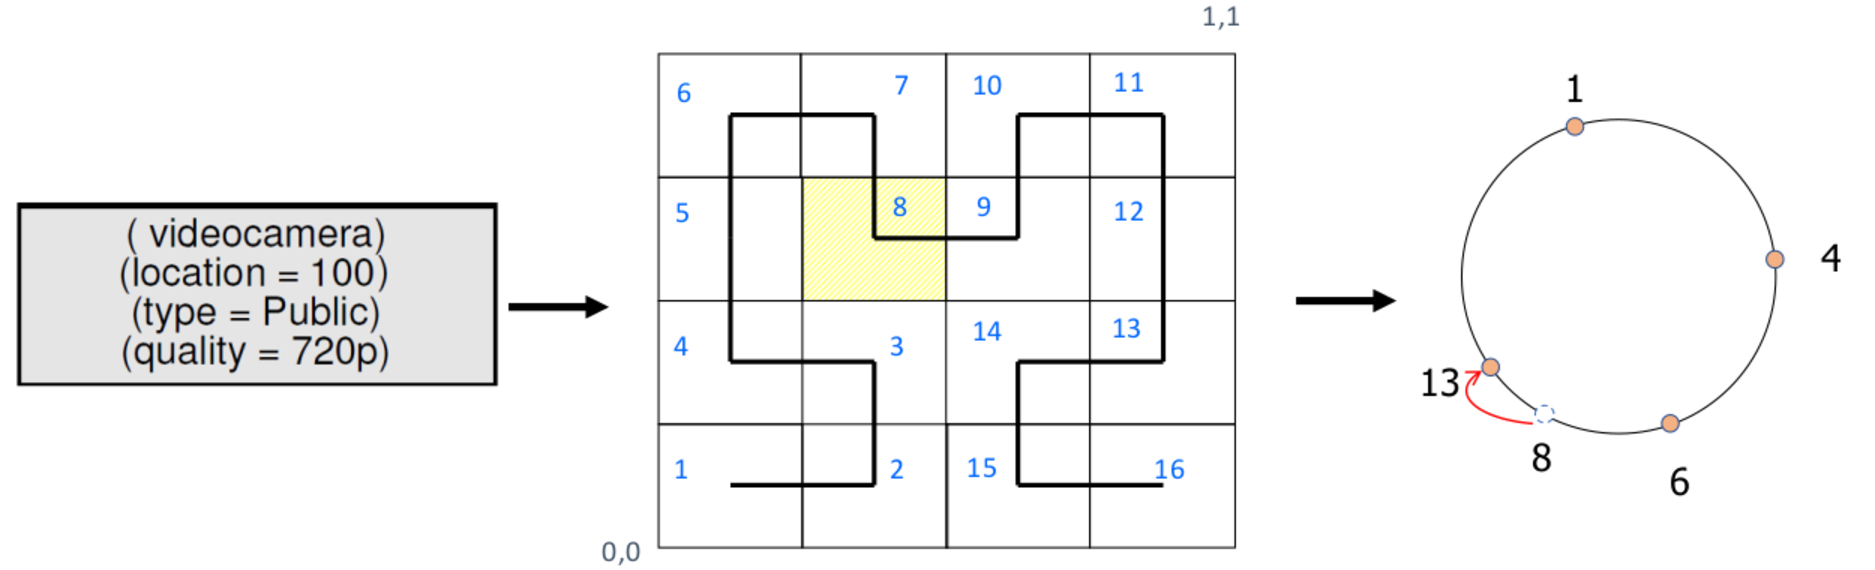
\includegraphics[width=1\linewidth]{Figures/single.pdf}
   \caption{}
\end{subfigure}
\begin{subfigure}[b]{0.9\textwidth}
   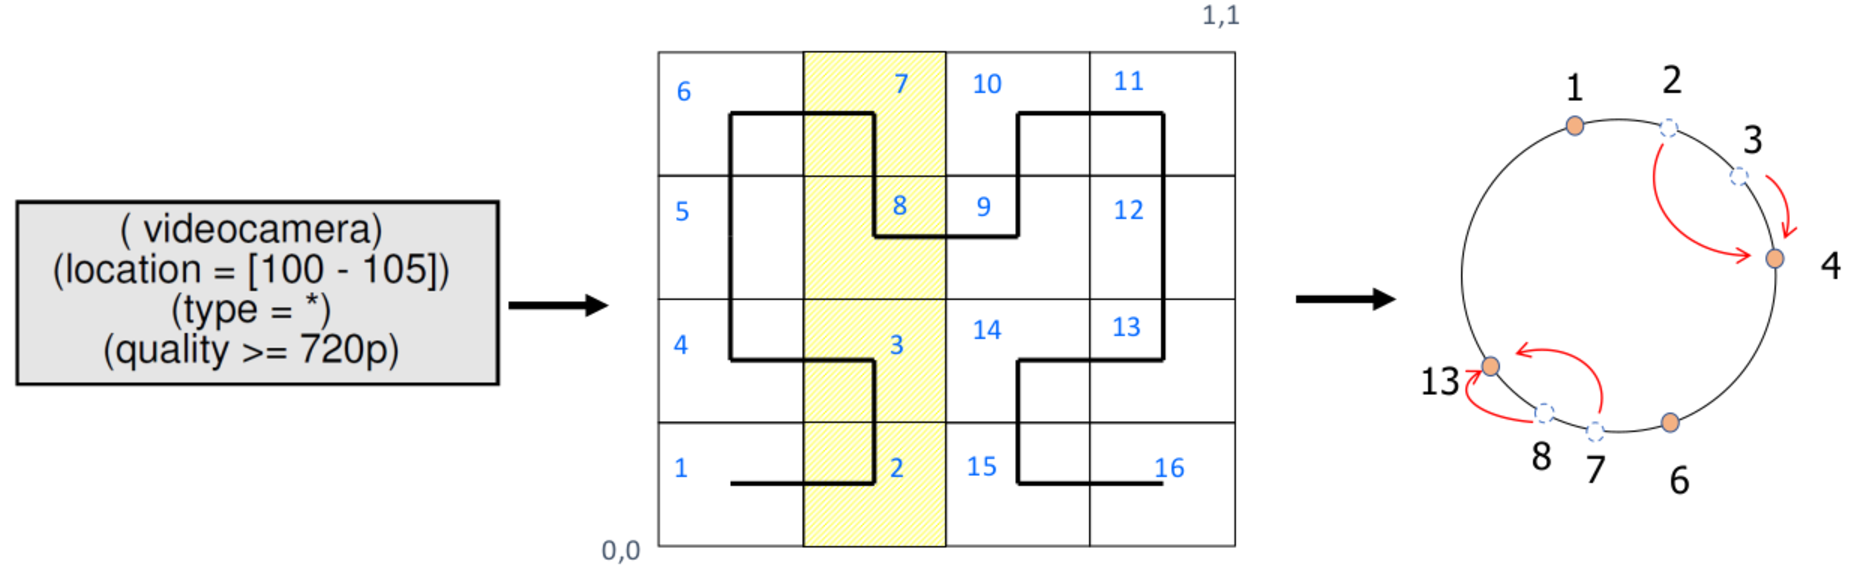
\includegraphics[width=1\linewidth]{Figures/multi.pdf}
   \caption{}
\end{subfigure}
\caption{R-Pulsar space filling curve routing using simple (a) and complex (b) profiles.}\label{fig:routingProfiles} 
\end{figure}

%As mentioned above, the lookup operator provided by the location-aware overlay requires an exact identifier, the AR message and the location to be routed.

This component builds on top of the location-aware overlay to route messages. The content-based routing component maps AR profiles onto single identifiers or clusters of identifiers to enable information discovery using partial knowledge, as described in \cite{SCHMIDT2008962}.

Content-based routing is achieved by performing two steps: The first step is to encode the set of attributes and/or attribute-value pairs of the AR message, into a set of unique base 10 ids. The second step is to use the set of base 10 numbers produced in the previous step and pass them to the Hilbert Space Filling Curve (SFC). The SFC~\cite{SFC} is used to map the n-dimensional space of the AR profile to the one-dimensional space ID of the location-aware overlay network. Content based routing can be performed in two ways using simple keyword profiles or complex keyword profiles, the routing process is described below.

\textbf{Routing using simple keyword profiles:} The routing process consists of two steps. At the first step, the AR profile containing only exact attribute-value pairs is encoded into a set of based 10 ID's, each id represents an exact attribute-value pair of the AR profile, then the set of base 10 ID's are passed to the SFC to obtain a single based 10 ID. This base 10 ID corresponds to 160bit unique identifier used by the P2P overlay network. Figure~\ref{fig:routingProfiles}a illustrates this process. \vspace{1ex} 

\textbf{Routing using complex keyword profiles:} Similarly to the first step, an AR profile this time contains wildcards, ranges, or both is encoded and a set of base 10 ID's. The wildcard gets replaced for each of the possible value in the alphabet, producing multiple base 10 encoding sets. This sets of encoding are passed to the SFC to obtain a single based 10 ID, this step is repeated for each of the base 10 encoding sets. Then we end up with muntiple base 10 IDs that corresponds to several 160bit unique identifiers of the P2P overlay network. Figure~\ref{fig:routingProfiles}b illustrates this process.


\section{Streaming Layer}

The streaming layer provides users and applications with efficient data-driven access to federated resources. This layer is composed of the serverless API, memory-mapped streaming analytics, and the rule-based programming components:

\subsection{Serverless API Component}\label{sec:serverless}

%\begin{figure}[!h]
%  \centering
%  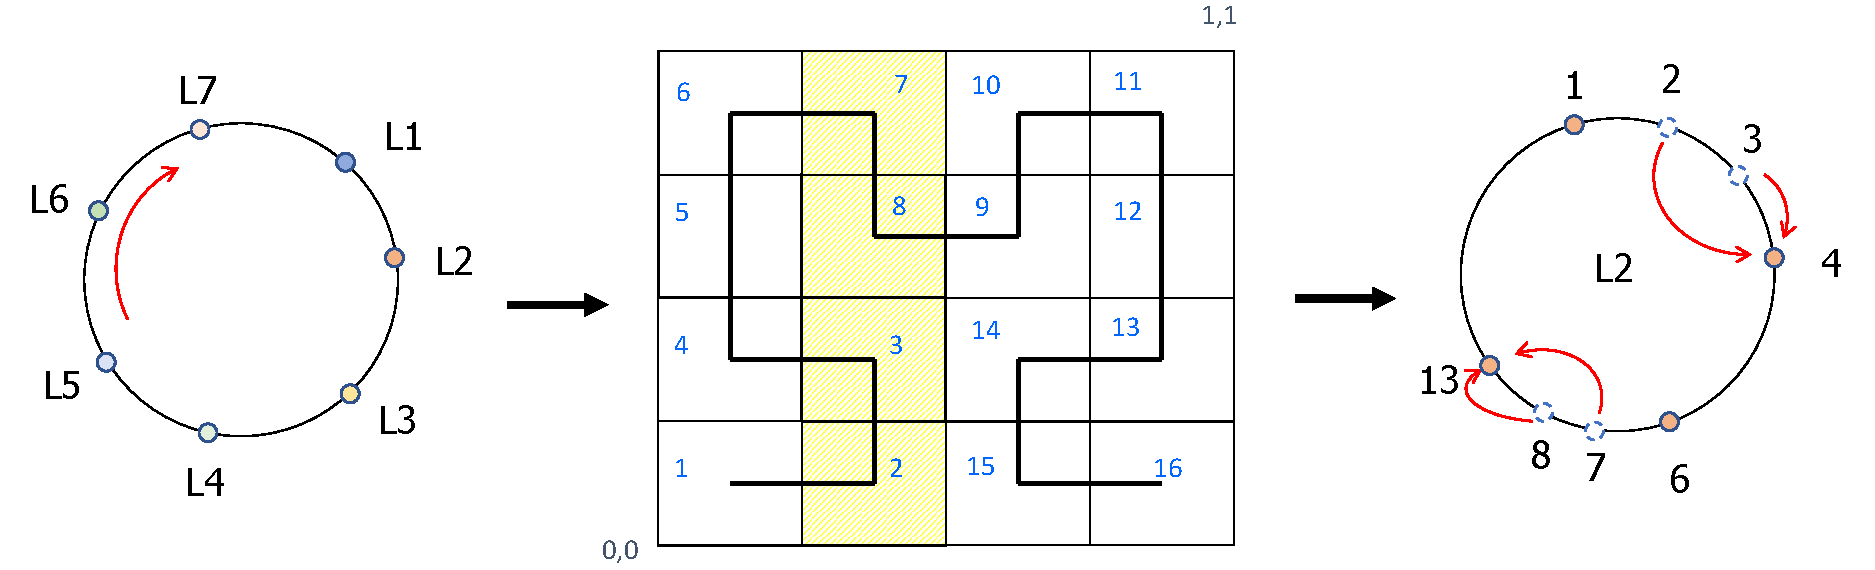
\includegraphics[width=0.9\columnwidth]{Figures/multi-old.pdf}
%  \caption{}\label{fig:Multiquad}
%\end{figure}

Serverless computing is a cloud computing model that aims to abstract server management and low-level infrastructure decisions away from developers. Allowing to deploy and execute pieces of code in response to events without the need to specify IP addresses. The serverless messaging layer implements the AR interaction model described in Chapter~\ref{chap:AR} and it consists of two components: the matching engine and the profile manager. 

The matching engine component is essentially responsible for matching profiles. If the result of the match is positive, then the action field of the incoming message is executed first, followed by the evaluation of the action field in the matched profiles. 

The profile manager manages locally stored profiles and monitors message credentials and contexts to ensure that related constraints are satisfied.

\begin{table}[h]
\caption{Available R-Pulsar operators.} \label{tb:operators}
\resizebox{\textwidth}{!}{%
\begin{tabular}{cc}
\hline
\textbf{Operators}                       & \textbf{Guarantees}                                                                                                                                                                                                    \\ \hline
bool \textbf{init()}                             & \begin{tabular}[c]{@{}c@{}}Connects to the existing P2P network \\ and guarantees the discover all existing RPs\end{tabular}                                                                                           \\ \hline
bool \textbf{post}(AR Message)                   & \begin{tabular}[c]{@{}c@{}}Routes the AR Message based on the \\  profile and the location;\\  Guarantees that all RPs responsible for that \\  content in that location will receive the \\  AR message.\end{tabular} \\ \hline
bool \textbf{stream}(AR Message, String Peer Id) & \begin{tabular}[c]{@{}c@{}}Stream direct messages to a select RP.\\ Guarantees that the responsible RP will\\ always receive the message.\end{tabular}                                                                 \\ \hline
AR Message \textbf{poll}()                       & \begin{tabular}[c]{@{}c@{}}Retrieve messages from a select RP point.\\ Guarantees that the consumer will always\\ receive the message.\end{tabular}                                                                    \\ \hline
\end{tabular}
}
\end{table}

The serverless messaging component offers four different operators. Table~\ref{tb:operators} summarized all of the available operators.

The \textbf{init}() operator is used to join the R-Pulsar network and it guarantees that all the available RPs will be discovered.

The \textbf{stream}(AR Message, String Peer Id) operator is used to stream data directly to a specific RP, this operator bypasses the location and the content based routing component.

The \textbf{poll}() operator is used to retrieve the data other RPs are sending.

The \textbf{post}(AR message) operator is used to route the messages without the need of specifying the recipient of the message, the recipient of the message is resolved by using the AR Message. To route a message using the post abstraction the following steps are performed:

\subsection{Memory-mapped Streaming Analytics Component}
The data pipeline is responsible for consolidating data from multiple sources, processing the data, and making them available to be used. State-of-the-art data pipelines are known to be data-intensive tasks, resulting in the inability to performing real-time data analytics when deployed on constrained devices. The memory-mapped streaming analytics pipeline component is motivated to overcome that issue. The streaming analytics pipeline comprises the following sub-components: 

\begin{enumerate}

\item The data collection layer gathers data from multiple sources and brings them to the pipeline.
\item The stream processing layer processes the data and performs computations on the collected data.   
\item The data storage and query layer reads and writes data to the main memory and disk.

\end{enumerate}

\subsubsection{Data Collection}

Multiple data collection services are available, such as Apache Kafka~\cite{kafka}, Google Pub/Sub~\cite{google}, Amazon Firehose~\cite{amazon}, and Mosquitto~\cite{mosquitto}. Although some are designed to be deployed on edge devices, these services offer limited performance when deployed in constrained devices due to the limited read and write disk speeds.

We designed and implemented a custom data collection sub-component designed specifically for constrained devices using a memory-mapped queue. A memory mapped file is a segment of virtual memory that has been assigned a direct correlation with some portion of a file. This file is physically present on disk, which allows the operating system to ensure data access operations with better performance than standard file access. The core principle of the R-Pulsar queue system emerges from the observation that random memory read is about 3.5x faster than sequential disk read, as measured in Table~\ref{tb:table1}. 

The trade-off of using a memory mapped data collection system is that operating systems decides when to copy data from the main memory to disk.  
\\
\begin{table}[h!]
\centering
\caption{Measurements of Disk I/O vs RAM memory performance on a Raspberry Pi.} \label{tb:table1}
\scalebox{1.2}{
\begin{tabular}{|l|c|c|}
\hline
\multicolumn{1}{|c|}{\textbf{Operation}} & \textbf{Disk} & \textbf{RAM Memory} \\ \hline
Sequential read                          & 18.89 MB/s             & 631.34 MB/s \\ \hline
Sequential write                         & 7.12 MB/s              & 573.65 MB/s \\ \hline
Random read                              & 0.78 MB/s              & 65.96 MB/s              \\ \hline
Random write                             & 0.15 MB/s              & 65.88 MB/s              \\ \hline
\end{tabular}}
\end{table}

\subsubsection{Data Processing }

R-Pulsar can be used on top of any data processing engine, allowing the end user to choose his or her favorite data-processing engine. The current release of R-Pulsar was validated using Apache Edgent. 

\subsubsection{Data Storage and Query}

This sub-component leverages the AR programming abstraction and a key-value database to offer SQL-like query capabilities. The storage sub-component uses the SFC of the content-based routing component to allow the ability to perform wildcard, range, or exact queries and allows the data to be horizontally partitioned among multiple RPs. 

For storing data, R-Pulsar relies on RocksDB~\cite{rocks}, an embedded key-value database optimized for fast and low-latency storage. The database keeps the most recently used data in the main memory and stores the least recently used data on disk.

\subsection{Rule-based Programming Abstraction}\label{sec:programming-data}
The rule-based programming abstraction makes it possible to build IoT applications and decide \textbf{when} data must be sent to the cloud for further postprocessing without having to manage any infrastructure.

It consists of a rule engine that allows developers to specify IF-THEN rules that can trigger other data-processing tasks when a condition is satisfied. The THEN clause of the conditions sends an AR message with a custom profile to start and stop data-processing tasks on demand. %The design and evaluation of the rule-based programming abstraction were illustrated in our previous paper~\cite{rules}.

We created a rule-based system, which contains all of the appropriate knowledge encoded into a set of If-Then rules. The system examines all the rule conditions (IF) and determines a subset, the conflict set, of the rules whose conditions are satisfied based on the data tuples. Out of this conflict set, one of those rules is triggered (fired). When a rule is fired, the action specified in its THEN clause is carried out. The loop for firing rules continues until one of two conditions are met: there are no more rules whose conditions are satisfied or a rule is fired. We allow to specify two different types of rules, ones that let you express data quality requirements which impose time constraints on the processing of the tuples, allowing the specification of a trade-off between the data quality and computational complexity. And the second one that offers the ability to express content-driven rules which complement the data quality requirements by triggering further stream-processing topologies either at the core or at the edge of the network if the data needs further processing due to quality of the data.

\subsubsection{Content-Driven Rules}
The content-driven rules consists of a single rule table that contains a set of rule entries installed by the developer. The rule entries contain a collection of conditions, a single action, and a single priority field.

The priority field is used in the event of having two or more rules that satisfy the condition, in order to brake the tie, only the one with highest priority will be executed. The condition field consists of one ore multiple antecedents (If clause). The antecedent of a rule consists of two parts: an object and its value. The object and its value are linked by an operator. The operator identifies the object and assigns the value. Table~\ref{tb:ruleOp} summarized all the rule operators currently supported.


\begin{table}[h]
\caption{Available R-Pulsar rule operators.}\label{tb:ruleOp}
\resizebox{\textwidth}{!}{%
\begin{tabular}{cc}
\hline
\textbf{Operator}                                                                                       & \textbf{Definition}                                                                                                                                                                                                                                                                                                                                                 \\ \hline
AND                                                                                                     & Evaluates if two values or expressions are both true.                                                                                                                                                                                                                                                                                                               \\ \hline
OR                                                                                                      & Evaluates if at least one of multiple values or expressions is true.                                                                                                                                                                                                                                                                                                \\ \hline
NOT                                                                                                     & Returns false for true and true for false.                                                                                                                                                                                                                                                                                                                          \\ \hline
\begin{tabular}[c]{@{}c@{}}\textgreater{},\textless{},\\ \textgreater{}=,\textless{}=\\ ==\end{tabular} & \begin{tabular}[c]{@{}c@{}}Evaluates if a value is less than the value that follows this symbol.\\ Evaluates if a value is greater than the value that follows this symbol.\\ Evaluates if a value is less than or equal to the value that follows this symbol.\\ Evaluates if a value is greater than or equal to the value that follows this symbol.\end{tabular} \\ \hline
MIN                                                                                                     & Returns true if the given number is the lowest number from a list of numbers.                                                                                                                                                                                                                                                                                       \\ \hline
MAX                                                                                                     & Returns true if the given number is the highest number from a list of numbers.                                                                                                                                                                                                                                                                                      \\ \hline
AVG                                                                                                     & Returns true if the given number is the avg number from a list of numbers.                                                                                                                                                                                                                                                                                          \\ \hline
STD                                                                                                     & Returns true if the given number is the std number from a list of numbers.                                                                                                                                                                                                                                                                                          \\ \hline
IF                                                                                                      & \begin{tabular}[c]{@{}c@{}}Determines if expressions are true or false. \\ Returns a given value if true and another value if false.\end{tabular}                                                                                                                                                                                                                   \\ \hline
\end{tabular}
}
\end{table}

The rule actions define what to do when the condition is satisfied, then the rule is fired and the action its performed. Each rule-entry has a single action associated with it; the three actions that are currently supported in our AR system are:

\begin{enumerate}
  \item \textbf{Store} the results of the computation at the Edge or the Cloud. This allows the topology developers to seamlessly store the results of the topology based on the content of the data across a federated set of resources and have the ability to locate where those data results have been stored when needed.
  \item \textbf{Trigger} a new Apache Storm topology, if it doesn't exist already, or route the tuples to an already running topology. Can be used to achieve multiple functionalities such as: split topologies/workflows across a set of participating Rendezvous Points that can be located at the core or at the edge of the network or make decisions based on the content of the data and triggering new computations.
  \item \textbf{Notify} action allows to notify any node part of the overlay network and stream the results to them.
\end{enumerate}

The rules can also be used to evaluate using a single tuple at a time or using window of tuples at a time. Windows is the concept in stream processing of splitting the infinite streams into finite chunks, and then apply computations to each chunk. There are two types of windows:

\begin{itemize}
    \item \textbf{Sliding Window:} tuples are grouped within a window that slides across the data stream according to a specified interval.
    \item \textbf{Tumbling Window:} tuples can be grouped in a single window according to a specified interval. Any tuple belongs to only one of the windows.
\end{itemize}

Windows can be specified accordingly to two different types of intervals: time and count.

Time can be used for sliding and tumbling windows to group elements from a given time period using the timestamp of the tuples. Count can be used for sliding and tumbling windows can be used to create windows with a defined size. In such a case, all windows will have the same size and the window will not be emitted if there are fewer elements than the defined size.

\begin{figure}[h!]
  \centering
  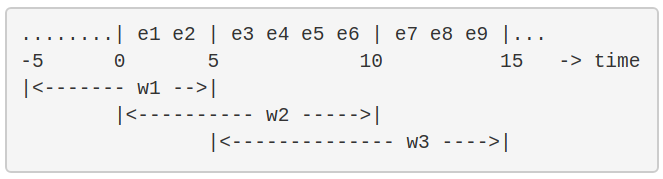
\includegraphics[width=0.7\textwidth]{Figures/SlidingWindow.png}
  \caption{A time duration based sliding window with length 10 secs and sliding interval of 5 seconds.}
  \label{fig:SlideBolt}
\end{figure}

Figure~\ref{fig:SlideBolt} depicts an example of a duration based sliding window with length 10 secs and sliding interval of 5 seconds. The window is evaluated every 10 seconds and some of the tuples in the first window overlaps with the second one. 

Figure~\ref{fig:TumbBolt} depicts a window is evaluated every five seconds and none of the windows overlap.

\begin{figure}[h!]
  \centering
  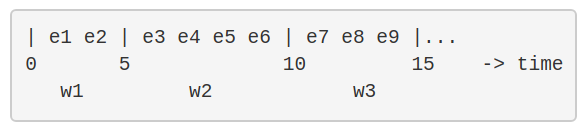
\includegraphics[width=0.7\textwidth]{Figures/TumblingWindow.png}
  \caption{A time duration based tumbling window with length 5 secs..}
  \label{fig:TumbBolt}
\end{figure}


\subsubsection{Data Quality Rules}

\begin{figure}[h!]
  \centering
  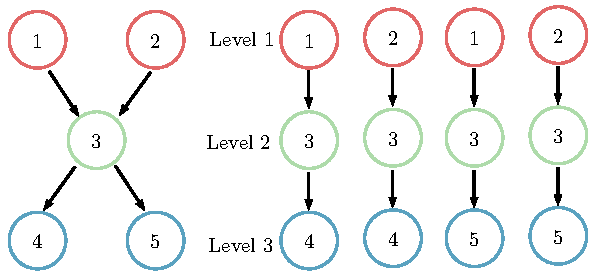
\includegraphics[width=0.6\textwidth]{Figures/AlgoImg.pdf}
  \caption{Storm topology linewise representation}
  \label{fig:AlgoImg}
\end{figure}

The second type of rule are the data quality rules. Data quality rules are used in workflows that have multiple redundant computations, where each computations takes different amount of time and produces a different data quality. The rule system is designed so users can specify time and data quality constraints so the QoS for the application can be meet.

The data quality rules are only supported when the Apache Storm engine is used, since it was build using Apache Storm. The content based rules consist of a custom Apache Storm stream grouping and the rule engine. In Apache Storm, part of defining a topology is to define how data is exchanged between components (how streams are consumed by the bolts). A Stream Grouping specifies which streams are consumed by each bolt. A stream grouping tells a topology how to send tuples between two components. The rule engine parses the given rule entries and computes all the possible paths that will satisfy the constraints specified by the rules. In order for the stream grouping to determine all the paths that will satisfy the constraints specified by the rules we developed in an offline training mode where the stream grouping collects execution information, transfers information, etc.. to determine all the paths that will satisfy the constraint. The data quality rule entries contain a tag filed and a deadline filed. The tag filed needs to be part of each of the tuples that needs to processed. The deadline filed specifies how much time each tuple with the corresponding tag has to go through the entire Storm topology. The algorithm consists of following steps: (1) breakdown the Storm topology into lines-paths from the task of the first level to the task of the last level through only one child on each level; (2) order lines according to their relative computing times $T_{comp}^l$. (3) iterate over the lines until one of the lines does not meet the deadline $D$ and schedule the work.

\begin{figure}[h!]
  \centering
  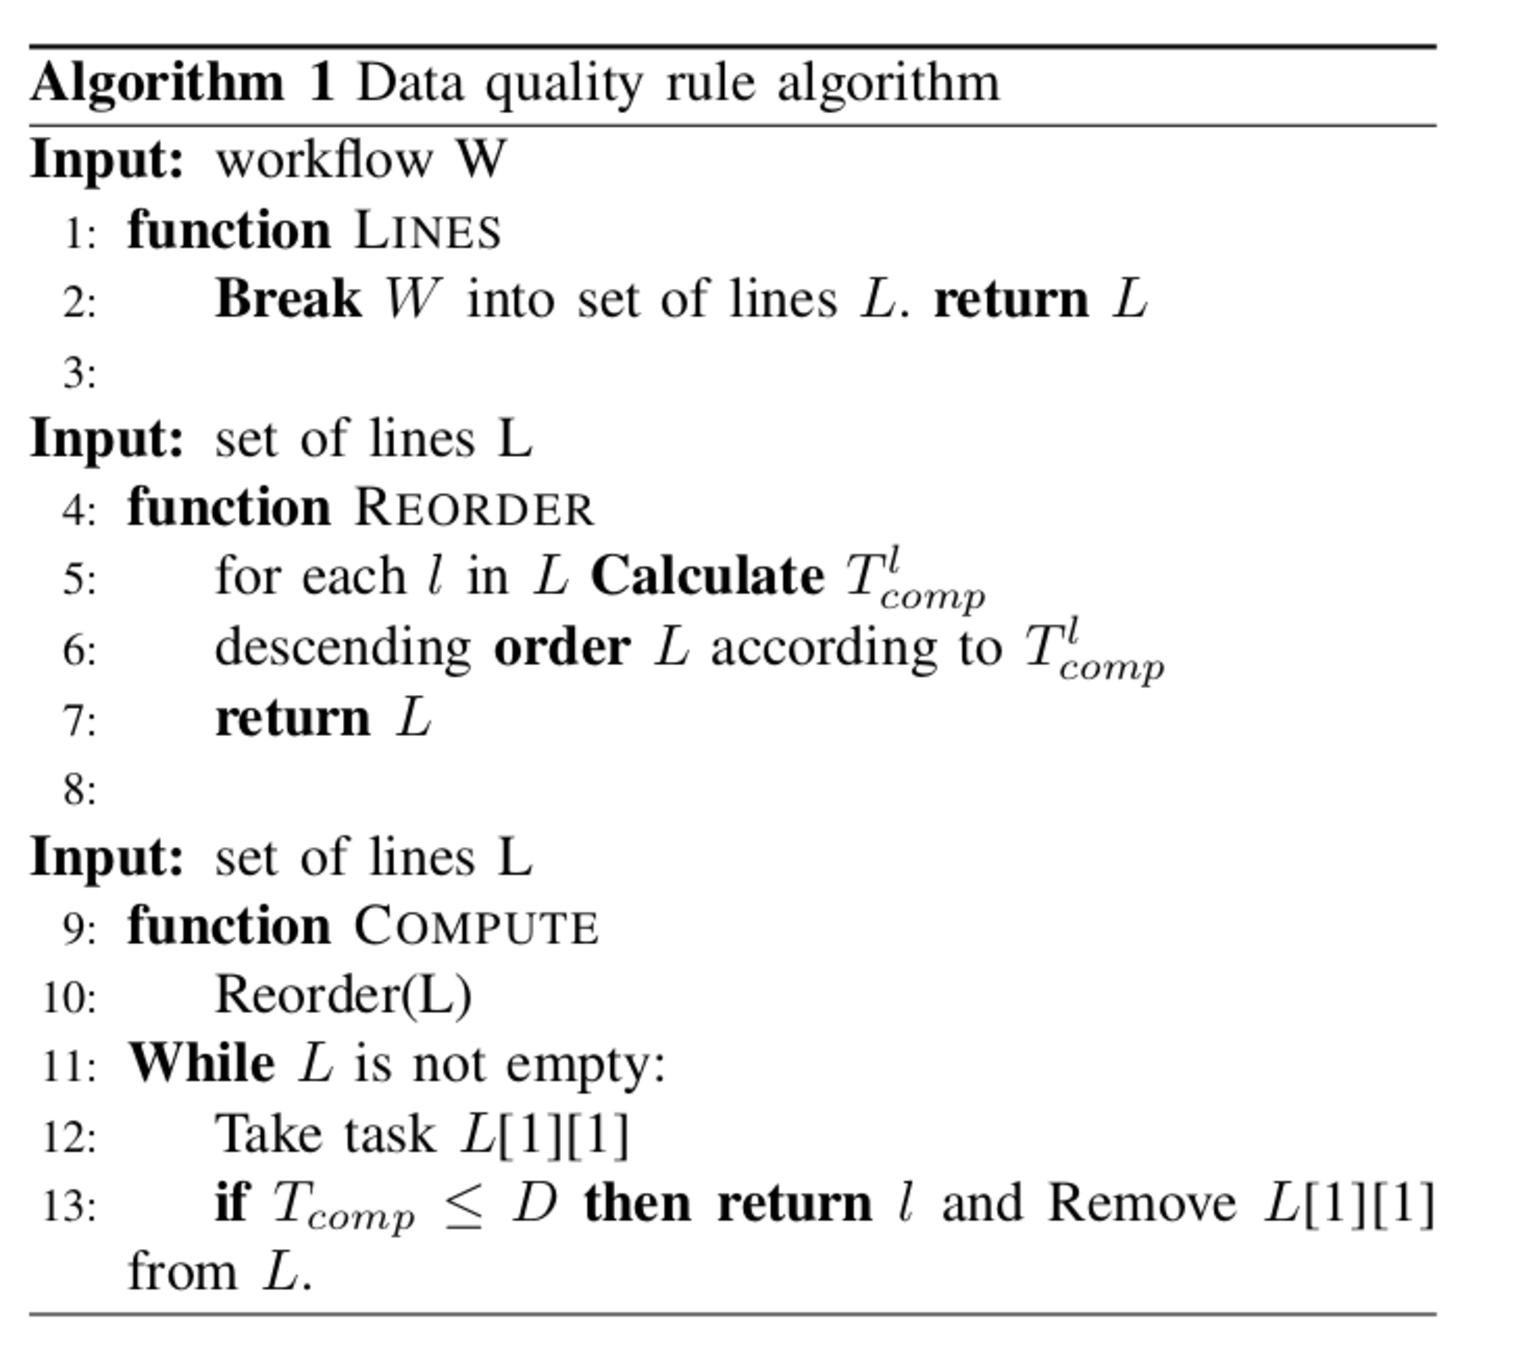
\includegraphics[width=0.7\textwidth]{Figures/Algorithm.pdf}
  \label{fig:Algorithm}
\end{figure}

The overall steps of the algorithm are depicted in Algorithm 1. In the first step of execution process the algorithm creates lines of the topology tasks and calculates the relative computing time $T_{comp}^l$ for each line. $T_{comp}^l$ is calculated as the sum of execution times $T_{comp}^l$ of all tasks in the line. $T_{comp}^l$ consists of task runtime $T_{run}^t$ and total input data transfer time $T_{data}^t$. Then we order all the paths according to their relative computing times $T_{comp}^l$ so we only need to check if $T_{comp}^l$ satisfies the deadline $D$. Once we find one path that does not satisfy the deadline $D$, we have our set of paths that satisfies the constraint and we schedule the work. The algorithm is constantly running and reschedules the work if the computation conditions change.

\section{Application Layer}

The application layer is composed of data consumers. Data consumers are the IoT applications described in Chapter~\ref{chap:applications}. Data consumers process these the incoming data from the sensors/data producers and aggregate incoming data, send automatic alerts in real-time, or produce new streams of data that can be processed by other consumers.
\chapter{Implementation of R-Pulsar}
\section{Introduction}

The current implementation of R-Pulsar build upon the open source project TomP2P. TomP2P is a P2P library and a distributed hash table (DHT) implementation which provides a decentralized key-value infrastructure for distributed applications. %Each peer has a table that can be configured either to be disk-based or memory-based to store its values. TomP2P stores key-value pairs in a distributed manner. To find the peers to store the data in the distributed hash table, TomP2P uses an iterative routing to find the closest peers. 

The overall operation of the R-Pulsar overlay network consists of two phases: bootstrap and running. During the bootstrap phase (or join phase), messages are exchanged between a joining RP and the rest of the group. During this phase, the joining RP attempts to discover RPs already existing in the system to build its routing table. The joining RP sends a discovery message to the group. If the message is unanswered after a set duration (in the order of seconds), the RP assumes that it is the first in the system and it becomes the master RP, creating a single overlay network (Peer-to-Peer network). Every time any other RP joins the overlay network and the master RP responds to the discovery message, the  RP is added to the system by using the location of the RP and determining which quadrant the RP occupies. Once the initial P2P network has a sufficient number of RPs to guarantee that in case of multiple failures the P2P network will not disappear, the quadtree subdivides the overlay network into four additional P2P rings, plus an extra ring that will allow all the master RPs of each ring to communicate. Each RP master keeps a copy of the quadtree, so in the case of an RP failure the overlay network structure will never be lost. In the case of a master RPs failure, a master RP election is performed using the Hirschberg and Sinclair algorithm~\cite{Hirschberg}.

The running phase consists of stabilization and user mode. In the stabilization mode, an RP responds to queries issued by other RPs in the system. The purpose of the stabilization mode is to ensure that routing tables are up to date and to verify that other RPs in the system have not failed or left the system. In the user mode, RPs allow external entities to use the serverless layer to communicate with each other to offer and request data and computation. These entities can include: a) users that might want to retrieve specific data or perform certain computation over data found using a query; b) IoT devices that can produce and consume data based on specific interests; and c) computational resources, such as data analytics and streaming platforms, clouds, or high performance computing clusters that offer their computational capabilities.

In addition the user mode is also responsible for replicating the data. R-Pulsar uses an indirect replication method which is inherited from TomP2P. The indirect replication can be described as peers publishing content for others. The peer closest to a location ID is considered as the responsible peer and replicates data if necessary. Doing so allows data to never be lost, data will only be lost in the unlucky event that all the RPs fail at the same time or not RPs are up.

\section{API Examples}
In this section, we present two sets of API examples based on the disaster recovery use case presented in Chapter~\ref{chap:applications}. They illustrate the use of R-Pulsar’s API for basic use of resource actions for sensor registration and discovery (Listing 1-2) and the use of function actions for storing and triggering data-processing tasks (Listing 3-5)

The first example uses the resource actions for enabling the exchange of data, without prior knowledge between devices. In Listing~\ref{lst:sensor}, an advertising profile is specified by the drone sensor with the type of data it can produce, and requests to be notified when someone is interested in such data.

\begin{lstlisting}[language=mylang, caption={Data producer resource profile sample code.}, captionpos=b, label={lst:sensor}]
1 profile.addSingle("Drone").addSingle("LiDAR");
2 ARMessage msg = ARMessage.newBuilder()
  .setAction(ARMessage.NOTIFY_INTEREST)
  .setLatitude(40.0583).setLongitude(-74.4056))
  .setProfile(profile);
3 producer.post(msg);
\end{lstlisting}

Respectively, a data consumer declares the type of content of its interest. Listing~\ref{lst:ed} presents a data consumer with interest for any LiDAR sensor data that match the profile ``Drone" and ``Li*", located within the specified range (40*, 70*). As this profile matches the previous profile, the sensor from Listing 1 is notified that there is a consumer interested in its data, then the sensor starts streaming.

\begin{lstlisting}[language=mylang, caption={Data consumer resource profile sample code.}, captionpos=b, label={lst:ed}]
1 profile.addSingle("Drone").addSingle("Li*")
  .addSingle("lat:40*").addSingle("long:-74*");
2 ARMessage msg = ARMessage.newBuilder()
  .setProfile(profile).setAction
  (ARMessage.NOTIFY_DATA);
3 producer.post(msg);
\end{lstlisting}

As mentioned previously, profiles can be used in two different ways: for discovering resources or subscribing to data publishers (resource actions) and for deploying data-processing tasks across the edge and the cloud (function actions). Listing~\ref{lst:ed2} implements the deployment of a function (post\_processing\_func) in the system. This allows the developer to specify where/on which set of resources it should be deployed.

\begin{lstlisting}[language=mylang, caption={Store post-processing task in the R-Pulsar overlay network.}, captionpos=b, label={lst:ed2}]
1 profile.addSingle("post_processing_func");
2 ARMessage msg = ARMessage.newBuilder()
  .setProfile(profile).setLocationTag("Cloud");
  .setAction(ARMessage.STORE_FUNCTION);
3 producer.post(msg);
\end{lstlisting}

Consequently, a profile and a decision (the IF-THEN rule) can be created to decide \textbf{when} to trigger the data-processing function (post\_processing\_func). In Listing~\ref{lst:t-rule}, the resulting action is created and attached to the function profile from Listing~\ref{lst:t-start2}, which is sent when the rule is satisfied.

In addition, Listing~\ref{lst:t-rule} defines a rule that is constantly evaluated for every data element. If the condition of this rule is met, then the function profile from Listing~\ref{lst:t-start2} is forwarded, resulting in the execution (trigger) of the data-processing task previously stored.

\begin{lstlisting}[language=mylang, caption={Rule based programming abstraction for deploying the post-processing task.}, captionpos=b, label={lst:t-rule}]
1 Action topo1 = new Reaction(T-profile);
2 Rule rule1 = new Rule.Builder()
  .withCondition("IF(RESULT >= 10)")
  .withConsequence(topo1).withPriority(0);
\end{lstlisting}

\begin{lstlisting}[language=mylang, caption={Profile for deploying the post-processing task.}, captionpos=b, label={lst:t-start2}]
1 T-profile.addSingle("post_processing_func");
2 ARMessage msg = ARMessage.newBuilder()
  .setAction(ARMessage.START_FUNCTION)
  .setProfile(T-profile);
3 producer.post(msg);
\end{lstlisting}

\section{Location-aware Overlay Network Layer Evaluation}

In this section we evaluate the overhead and scalability of the location-aware overlay network layer of R-Pulsar. The tests are evaluated using cloud and edge resources:

\begin{itemize}
\item Edge System:  Chameleon Cloud~\cite{chameleon}, a configurable experimental environment for large-scale cloud research~\cite{chameleon} with 100 instances of type m1.small (1 CPU and 2 GB RAM) to simulate the computation capabilities of a Raspberry Pi.

\item Cloud System: Using Chameleon Cloud~\cite{chameleon} with 100 instances of type m1.medium (2 CPU and 4 GB RAM).
\end{itemize}

\subsection{Overhead and Scalability Over Cloud And Edge Systems}

This experiment measures the overhead involved in performing a location-based query to identify relevant resources around the location of a client node. In our experiments, the location-based query used the GPS coordinates of each RP node and the client to identify the RP around the client. Not that for this experiment we did not deploy 500k RPs, we only used the location of 50k RPs to perform the queries.

\begin{figure}[htb!]
  \centering
    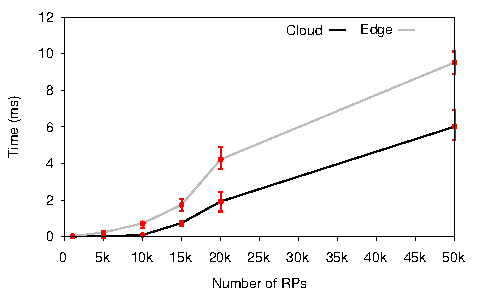
\includegraphics[width=0.8\textwidth]{Figures/OSLocation.pdf}
  \caption{Location-based query overhead for different number of matches per query.} \label{fig:oslocation}
\end{figure}

Figure~\ref{fig:oslocation} shows that the overhead of performing a location-based query increases as the number of RP nodes in the system increases. Results show a maximum overhead of 10 milliseconds, which occurred when 50k RPs are in the system. 

\subsection{Overhead and Scalability of the Data Replication}

Next, we measured the time required to replicate the information stored across a set of RP nodes in the system. In these experiments, we considered several scenarios involving different number of RP nodes as well as different number of replication factors. For this experiment we did deploy 25, 100 and 500 RPs, for the 5 RPs where deployed in the same instance in order to achieve 500 RP instances. Figure~\ref{fig:topology} collects the results. 

\begin{figure}[htb!]
  \centering
    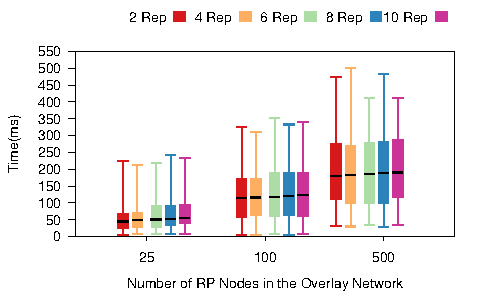
\includegraphics[width=0.8\textwidth]{Results/ReplicationOver.pdf}
  \caption{Time neccessary to update information of all RP nodes in the system after multiple topologies are registered.} \label{fig:topology}
    \vspace{-2ex}
\end{figure}

We can observe that in Figure~\ref{fig:topology} that the time required to replicate the information across all the RP nodes in the system is relatively low. In particular, it can vary from a few milliseconds to around 200 milliseconds on average when having a large system with 500 RP nodes. The main factor affecting the time required to propagate the information is the number of RP nodes, since the time to route a message increases. 

\section{Content-based Routing Layer Evaluation}

In the content-based routing layer we evaluate three aspects: The first aspect is the overhead of matching profiles, The second aspect we evaluate is the overhead and scalability of the routing, and finally we evaluate the time it takes to propagate information through the system when a new RP joins the system. The tests are evaluated using the same cloud resources as described in the previous section. For the edge resources of this set of experiments we used two different setups:

\begin{itemize}
\item Raspberry Pi System: Using 2 Raspberry Pi's 3 with 4x ARM Cortex-A53 1.2GHz, 1GB LPDDR2 of RAM and 10/100 Ethernet.

\item Android System: Using 1 Motorola Moto G5 Plus with a Qualcomm Snapdragon 625 processor with 2.0 GHz octa-core CPU, 3GB of RAM
\end{itemize}

\subsection{Profile Matching Overhead Over Cloud Systems}

This first experiment measures the overhead involved in the profile matching operation at an RP node. We used a {\it notify\_data} action message for these experiments. We considered different scenarios in which the system had different number of data profiles (i.e. subscriptions) and the request returned a different number of profile matches. %As we described in Figure~\ref{fig:example1B}, a {\it notify\_data} request asks an RP to find matching profiles and to send a {\it notify} message to the profile owners -- e.g., requesting to start streaming data. In this experiment, we measured the overhead of performing the matching operation and constructing the ``notify'' messages.  
The experiment was conducted using profiles that contained complex keyword tuples, wildcards and/or ranges. Figure~\ref{fig:profileQuery} collects the results of these experiments. 

\begin{figure}[htb!]
  \centering
    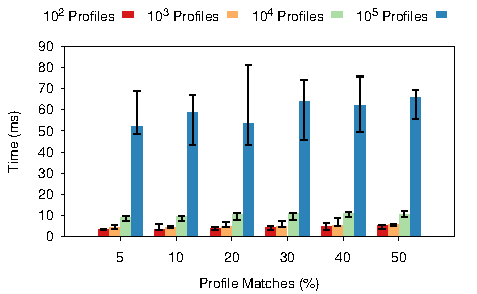
\includegraphics[width=0.8\textwidth]{Figures/profileQuery.pdf}
  \caption{Profile matching overhead. Results are grouped based on the matching ratio expressed as a percentage of the total number of stored profiles.} \label{fig:profileQuery}
\end{figure}

We can observe in Figure~\ref{fig:profileQuery} that, for a moderate database size of up to $10^4$ profiles, the profile-matching operation incurs in an overhead between five and 10 milliseconds. Nonetheless, when we increase to $10^5$ profiles, the overhead increases significantly, as could have been expected given the memory and data access times required to identify and retrieve such a large number of profiles.

\subsection{Routing Overhead and Scalability Over Edge Systems}

This second set of experiments measure the routing overhead, which represents the time interval between an AR message is created until it is forwarded to the recipient of the message. It is important to maintain the routing overhead in the order of milliseconds to achieve real-time analytics on constrained devices. The routing overhead was evaluated over Android and Raspberry PIs by simulating the storage or retrieval of data, as the number of RPs on a given region grows, and also as the AR profiles complexity grows. The profile complexity is defined in terms of the number of attribute-value pairs that make up the profile. For example, a 2D profile is composed of two properties, such as data type and location.

\begin{figure}[h!]
  \centering
  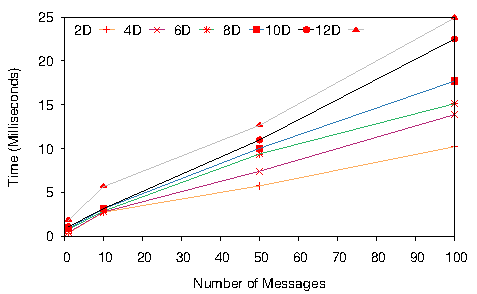
\includegraphics[width=0.8\textwidth]{Results/Phone}
  \caption{Evaluation of R-Pulsar space filling curve routing overhead and scalability as the number of messages and the complexity of profiles increase over the Android system.}
  \label{fig:Phone}
\end{figure}

\begin{figure}[h!]
  \centering
  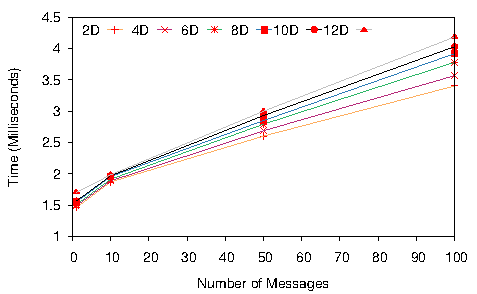
\includegraphics[width=0.8\textwidth]{Results/Raspberry}
  \caption{Evaluation of R-Pulsar space filling curve routing overhead and scalability as the number of messages and the complexity of profiles increase over the Raspberry Pi system.}
  \label{fig:Raspberri}
\end{figure}

Figure~\ref{fig:Phone} shows that when the profile complexity increases by a factor of 6, the time required to route messages increases by 2.5. Similarly, when the system increases the number of messages sent by a factor of 100, the time required to route one message increases by a factor of 25. It shows that the routing overhead scales efficiently in both cases, as messages become increasingly complex and as the number of messages sent increases when using the Android system. 

However, Figure~\ref{fig:Raspberri} shows that when the profile complexity increases by a factor of 6, the time required to route messages increases by about 1.2, when using the Raspberry Pi system. Likewise, when the system increases the number of messages sent by a factor of 100, the time required to route one message increases by about 2.5. Demonstrating that the routing overhead scales more efficiently on a Raspberry Pi system than on an Android system.

\subsection{Information Propagating through the System}

This experiment is performed to understand the behavior of the system when multiple RP nodes request to join an existing deployment of our system. Specifically, we measured the time from when the RP nodes sent their joint message until all RP nodes existing in the system were updated. In our experiments, we varied both the number of RP nodes wanting to join and the number of existing RP nodes in the system. Figure~\ref{fig:rpDiscovery} collects the results.

\begin{figure}[htb!]
  \centering
    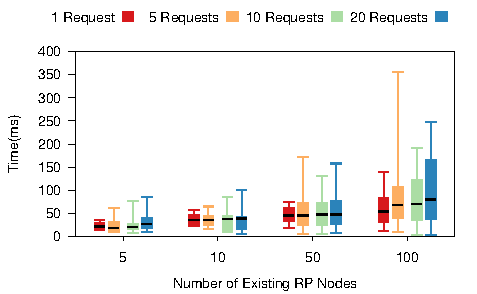
\includegraphics[width=0.8\textwidth]{Figures/rpDiscoveryBox.pdf}
  \caption{Time neccessary to update information of all RP nodes in the system after multiple new RP nodes join.} \label{fig:rpDiscovery}
\end{figure}

Figure~\ref{fig:rpDiscovery} shows that the time required to have a consistent view of all the new RP nodes after the requests are placed is relatively low, and that it scales properly when increasing the number of existing RP nodes. In the case of a small system with only five existing RP nodes the overhead is around 20 milliseconds on average. The overhead increases to around 70 milliseconds in the case of having a large system with 100 existing RP nodes. Additionally, we can observe that varying the number of requests does not significantly affect the time required to propagate the information in a system with up to 50 RP nodes. In the case of having 100 RP nodes, we observe that increasing the number of requests, increases the overhead as well as the dispersion around the average. Although it is important to maintain an updated view of the system to ensure that we can efficiently process clients' requests, it is not critical for the regular operations of the system. Our system has mechanisms to adapt to changes in the availability of RP nodes to improve data processing efficiency. Therefore, we consider that having an eventually consistent system is sufficient. 

\section{Serverless Messaging Layer Evaluation}

\section{Memory-mapped Streaming Analytics Pipeline Evaluation}

In this section we evaluate two of the layers that the memory-mapped streaming analytics pipeline consists, the Data collection and the storage and query layers. The tests are evaluated using the same cloud resources as in the location-aware overlay network layer evaluation section. For the edge resources this set of experiments use the same as the content-based routing layer evaluation section. 

\subsection{Performance of the Data Collection Layer Over Edge Systems}

The first experiment aims to evaluate the throughput of R-Pulsar messaging layer. This experiment was carried out using two Raspberry Pi's one as a producer and the other as the broker. The workload sizes are chosen based on the current limitations imposed by existing IoT services, such as AWS~\cite{AWS-MQTT} and Azure~\cite{AZURE-MQTT}. The inner memory-mapped queue is compared to Apache Kafka and Mosquitto. Apache Kafka (the \textit{de facto} standard for cloud and edge data analytics)~\cite{Young2017, firework, planner}, Mosquitto (a broker that can be found on edge frameworks, such as Azure IoT or the AWS Greengrass), and the R-Pulsar memory-mapped queue, using four different message sizes.  The main difference between them is the way they store information: Apache Kafka and Mosquitto store messages on the disk while R-Pulsar stores them in the main memory and disk. 

\begin{figure}[h]
  \centering
  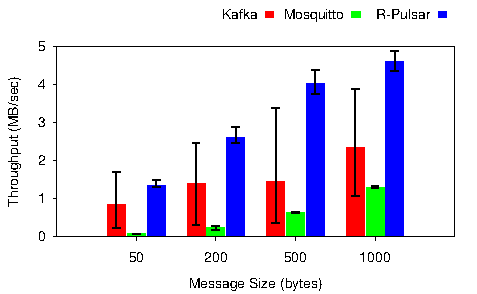
\includegraphics[width=0.8\textwidth]{Results/ProducerBar}
    \caption{Single broker and producer throughput performance as message sizes grow. Comparison of R-Pulsar, Kafka, and Mosquitto systems deployed on a single Raspberry Pi.}
  \label{fig:ProducerBar}
\end{figure}

Results in Figure~\ref{fig:ProducerBar} show that R-Pulsar's throughput scales as the message size increase. This experiment is representative of a traditional IoT scenario with small messages streamed at a high rate arrival.
We observed that R-Pulsar pub/sub messaging system outperforms Kafka by a factor of 3x and Mosquitto by a factor of 7x. Also, Apache Kafka exhibits a high variability of throughput performance. This is explained by the fact that Kafka continuously stores messages on the disk overwhelming the filesystem and producing this unpredictable throughput.
The use of a memory-mapped queue allows R-Pulsar to obtain higher throughput, but also steadier and more predictable throughput.

In this second experiment, we want to demonstrate that R-Pulsar can be deployed on  Android Phones. The experiment setup consists of an Android device as a data producer and a single Raspberry Pi as the RP. In Figure~\ref{fig:ProducerPhone}, the throughput comparison of R-Pulsar and Mosquitto~\cite{mosquitto} shows similar performance with larger messages. For smaller messages, R-Pulsar exhibits a better performance (factor of 10x). Also, Mosquitto presents a larger variability of performance (unpredictable throughput).

\begin{figure}[h!]
  \centering
  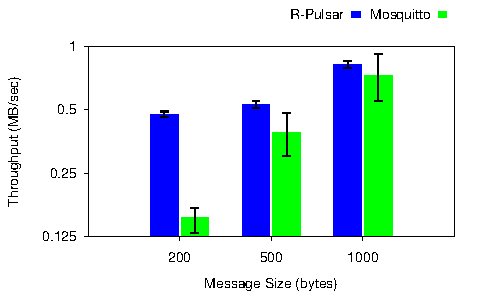
\includegraphics[width=0.8\textwidth]{Results/ProducerPhone}
  \caption{Single broker and producer throughput performance as message sizes grow. Comparison of R-Pulsar and Mosquitto on the Android system.}
  \label{fig:ProducerPhone}

\end{figure}

\subsection{Scalability of Store/Query Operations Over Cloud Systems}

These experiments are aimed to stress the system and evaluated the storage and query scalability of R-Pulsar using multiple workload sizes. The following workloads were used for the tests: Workload 1 (W1) stored/queried one element, Workload 2 (W2) stored/queried 10 different elements, Workload 3 (W3) stored/queried 50 different elements, and Workload 4 (W4) stored/queried 100 different elements. For this test, all RP nodes were part of the same P2P network and the same geographic region to evaluate how R-Pulsar scales as the number of RP increases in each region. 

\begin{figure}[h!]
  \centering
  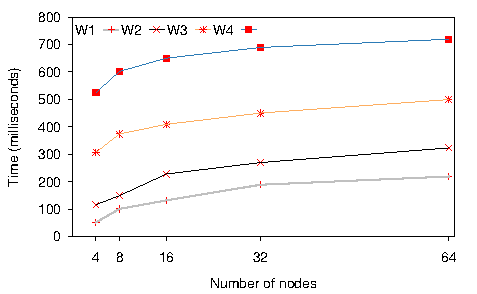
\includegraphics[width=0.8\textwidth]{Results/ProducerLine.pdf}
  \caption{Evaluation of R-Pulsar store query operations as the number of nodes increases on Chameleon cloud.}
  \label{fig:ProducerLine}
\end{figure}

Figure~\ref{fig:ProducerLine} presents the scalability evaluation of the R-Pulsar store operation. The figure shows that for storing a single element (W1), the runtime increased by a factor of $\sim$4 when the system size increased by a factor of 16 (from 4 nodes to 64 nodes). As the system expands, the number of intermediary nodes involved in routing the query grows, causing an increase in the runtime. The storage of 100 different elements (W4) forces the system to store elements in multiple destinations.

\begin{figure}[h!]
  \centering
  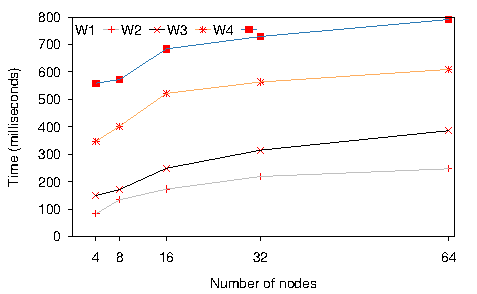
\includegraphics[width=0.8\textwidth]{Results/ProducerLineEx.pdf}
  \caption{Evaluation of R-Pulsar exact query operations as the number of nodes increases on Chameleon Cloud.}
  \label{fig:ProducerLineEx}
\end{figure}

Figure~\ref{fig:ProducerLineEx} presents an evaluation of the exact query operations. It shows that the query of a single element (W1), the runtime increases by a factor of 2.8 when the system size increases by a factor of 16 (from 4 nodes to 64 nodes).

\subsection{Performance of the Query and Store Layer Over Edge Systems}

The next set of experiments explores the performance of the R-Pulsar's storage and query layer as compared to self-contained, embedded and lightweight data storage systems. We compare R-Pulsar with lightweight SQL (SQLite) and non-SQL (NitriteDB) storage systems. We choose SQLite and Nitrite DB because  both systems are designed to be deployed in constrained devices~\cite{sqlite}~\cite{nitrite}. In addition, Nitrite DB is a key-value store like R-Pulsar. 

The experiments were deployed in 10 Raspberry Pis and grouped them together in the same R-Pulsar group. A client then issued requests for data to be stored and queried. As neither Nitrite DB nor SQLite supports horizontal data partitioning, the client directly queried a single DB for these systems. In the case of R-Pulsar, the content-based routing layer is responsible for determining where the data should be stored or queried.

We present three different results for these experiments. Figure~\ref{fig:DBInsertBar} shows the time required for each system to store different sets of elements. R-Pulsar presents a steady performance as the number of elements grows. It also outperforms Nitrite DB (factor of 30x).

\begin{figure}[h!]
  \centering
  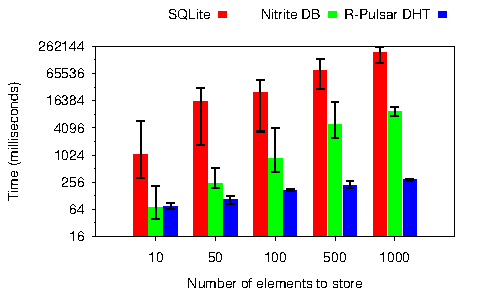
\includegraphics[width=0.8\textwidth]{Results/DBInsertBar}
  \caption{Storage performance of R-Pulsar, SQLite and Nitrite DB as the number of elements to be stored increases over 10 Raspberry Pi.}
  \label{fig:DBInsertBar}
\end{figure}

Figure~\ref{fig:DBExactBar} and~\ref{fig:DBWildBar} present the results for experiments using exact and wildcard queries (a profile containing wildcards, ranges or both).
In the last two experiments, we can observe that Nitrite DB and SQLite are both faster when the number of consecutive reads is small, but R-Pulsar outperforms both when the workload increases. Overall, R-Pulsar has a higher performance because it takes advantage of the distributed storage of data over multiple RPs so that queries can be performed in parallel.

\begin{figure}[h!]
  \centering
  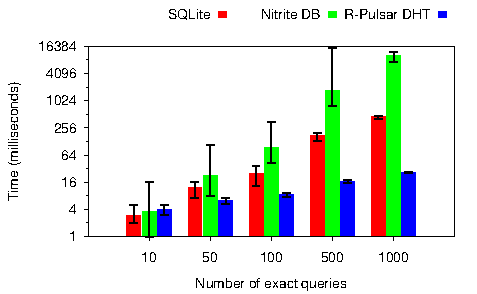
\includegraphics[width=0.8\textwidth]{Results/DBExactBar}
  \caption{Exact query performance of R-Pulsar, SQLite and Nitrite DB as the number of exact queries increases over 10 Raspberry Pi.}
  \label{fig:DBExactBar}
\end{figure}

\begin{figure}[h!]
  \centering
  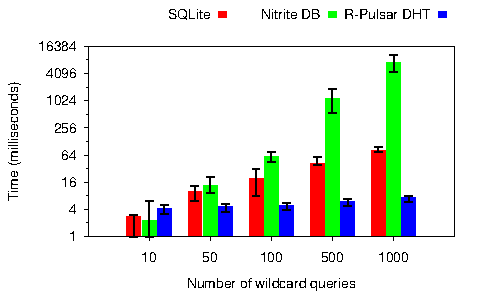
\includegraphics[width=0.8\textwidth]{Results/DBWildBar}
  \caption{Wildcard query performance of R-Pulsar, SQLite and Nitrite DB as the number of wildcard queries increases over 10 Raspberry Pi.}
  \label{fig:DBWildBar}
\end{figure}


\section{Rule-based Programming Abstraction Evaluation}

In this section we performed two sets of experiments to evaluate the rule-based programming abstraction. The tests are evaluated using two types of virtual nodes. The first node is our "drone" with computational capabilities with 1 vCPU and 2 GB of memory, we used a low CPU machine to simulate the overheads as if we used a small IoT device with reduced computational capacity. The second node is the "minivan" with 8 vCPU and 32 GB of memory.

\subsection{Scalability and Overhead Over Edge and Cloud Systems}

To evaluate the scalability and overhead of the rule engine system we added different rule amounts and streamed our regular workload, forcing the evaluation of each of the tuples. The plotted graph in Figure  \ref{fig:RuleEngine} shows the scalability and overhead of our rule engine for two different machines described above. We can observe that the overhead is very minimal and can be used for processing real-time stream processing, we can also observe that as we add rules the overheads do not increase exponentially making it suitable to handle hundreds of rules.

\begin{figure}[h!]
  \centering
  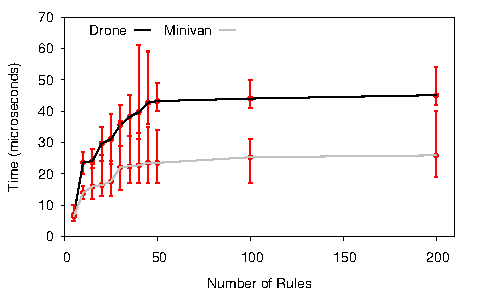
\includegraphics[width=0.8\textwidth]{Results/RuleEngine}
  \caption{Rule engine overhead for different number of rules.}
  \label{fig:RuleEngine}
\end{figure}

In this experiment we wanted to show the importance of being able to programmatically express a trade-off between data quality and computational performance. Figure \ref{fig:QoS} we demonstrate that if we do not allow the to specify QoS rules to set a deadline in this case a deadline of 20 seconds per tuple was specified, depending on the workload and the underlying computing capabilities most of the tuples will not satisfy the deadline. We can also see that our algorithm can't guarantee 100\% completion in time in small computational resources, but that is due to the fact that the CPU can't drain the storm bolt queues fast enough, so some tuples will experience some extra delay.

\begin{figure}[h!]
  \centering
  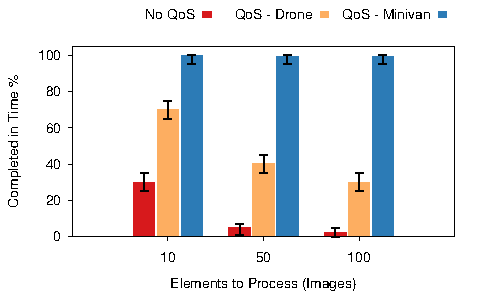
\includegraphics[width=0.8\textwidth]{Results/QoS}
  \caption{Data quality rule-based system 20 second deadline.}
  \label{fig:QoS}
\end{figure}

\section{End To End Evaluation}
In this section we implement two of the five uses cases using R-Pulsar to showcase the ability to express and decide what, where and when data gets collected and processed, using edge and cloud resources, and we compared it against a traditional approach of moving all the data to the cloud for analysis.

\subsection{Disaster Response Use Case}

For the disaster response use case we performed a set of experiments to compare the proposed split architecture (edge and core processing) with the current state of the art approach in which the stream processing is located in a fixed location at the core of the infrastructure. To perform these experiments we deployed them all in the same Chameleon cluster and we introduced artificial latency between the edge of the network and the core of the network. For the edge setup, 3 instances of type m1.small simulate computation capabilities of a drone (1 VCPUs and 2 GB of memory) and 3 other instances of type m1.medium simulate the minivan (2 VCPUs and 8 GB of memory). The core of the network is represented by 3 instances of type m1.large (4 CPUs and 8 GB of memory). To simulate that the edge infrastructure was located in a minivan or a drone we stored all the images that need to be processed locally to simulate a small latency since the minivan or the drone will be producing the data. For the traditional approach the storm topology gets the data from an external server to simulate the latencies need it to transfer between the edge and the core of the network.

\begin{figure}[h]
  \centering
  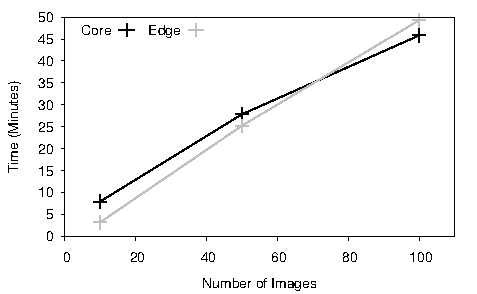
\includegraphics[width=0.8\textwidth]{Results/EdgeVCore}
  \caption{Disaster response workflow edge vs core no QoS.}
  \label{fig:Edge_CoreVsCloud}
\end{figure}

For the experiment in Figure \ref{fig:Edge_CoreVsCloud} we wanted to demonstrate that if we simply deployed our entire workflow at the edge of the network without any "quality" trade-off and we compared it to the traditional approach where each of the LiDAR images will be sent to the core for processing. We can see that with small workflows the edge is significantly faster than the core of the network, but as the number of images that need to be processed grows (the affected area is large) the core performs better than the edge due to limited resources at the edge of the network.

\begin{figure}[h!]
  \centering
  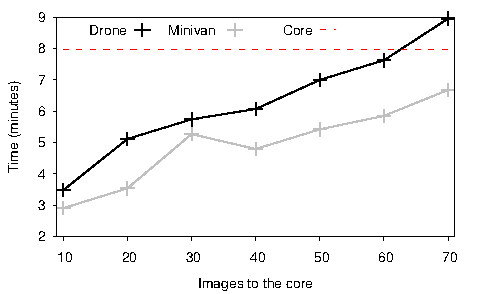
\includegraphics[width=0.8\textwidth]{Results/SmallSpeed}
  \caption{Disaster response workflow 10 images edge speed-up.}
  \label{fig:SmallSpeed}
\end{figure}

\begin{figure}[h!]
  \centering
  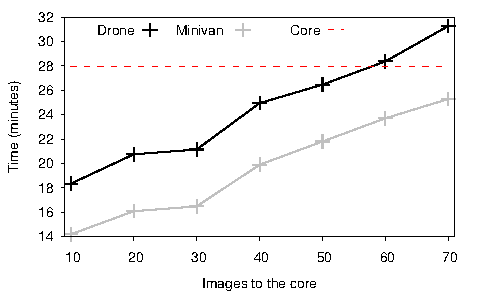
\includegraphics[width=0.8\textwidth]{Results/MediumSpeed}
  \caption{Disaster response workflow 50 images edge speed-up.}
  \label{fig:MediumSpeed}
\end{figure}

\begin{figure}[h!]
  \centering
  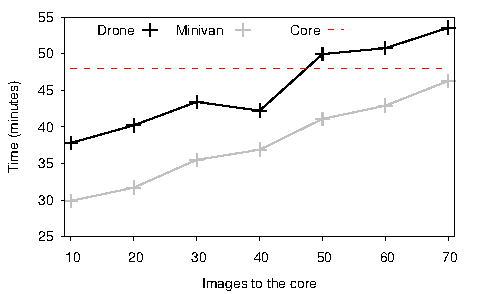
\includegraphics[width=0.8\textwidth]{Results/BigSpeed}
  \caption{Disaster response workflow 100 images edge speed-up.}
  \label{fig:BigSpeed}
\end{figure}

Figures \ref{fig:SmallSpeed} \ref{fig:MediumSpeed} \ref{fig:BigSpeed} showcase the speed-up that can be obtained by trading off some image "quality" for some computational complexity. Figure \ref{fig:SmallSpeed} is the graph for a workflow with 10 LiDAR images to be processed; one can observe that if we perform all the computations in the "drone" and only 10\% of those images need further processing we get a speed up of 44\% compared to sending all 10 images to the core of the network. We can observe from figures \ref{fig:MediumSpeed} \ref{fig:BigSpeed} that due to the small compute limitations, the drone gets a faster speed-up when the worflow size is small and a small percentage of tuples needs further processing, which makes it perfect for assessing affected areas where minivans can't get to due to road blocks. In the case of the minivan, it gets a higher speed-up in all three cases since it has higher computational resources and we can also observe that we can still send a large percentage of rules to the core and we still get a higher speed-up. In the best case the minivan is 71\% faster than the traditional approach where all the images are sent to the cloud.

\subsection{Smart City Use Case}

For the smart city use case we performed a set of experiments to compare the proposed edge stream processing approach with a traditional approach in which the stream processing is located in a fixed location at the core of the infrastructure. To perform these experiments we deployed two streaming frameworks (based on Apache Kafka plus Apache Storm), one in our local cluster and another one in Amazon AWS. In both cases, Apache Kafka and Storm were deployed in a single machine to avoid any additional latency due to communication across machines of a Kafka or Storm cluster. In Amazon AWS, we used an instance of type  t2.2xlarge, which has similar characteristics to the machines in our local cluster (8 CPUs and 32 GB of memory). Note that we do not assume that the edge will be equipped with similar characteristics, we are only using this type of instance for computational comparison only. When using our approach, our framework was deployed across both infrastructures -- i.e. we had two RP nodes exposing the capabilities of each stream engine. We emulated a scenario inspired by the one described in Chapter~\ref{chap:applications} in which a client performs a request to obtain navigation indications. The data-processing workflow (i.e. topology) was composed by three sequential steps (i.e. bolts in Apache Storm terms) that performed some basic data transformations that did not require significant computational time. In our experiments we evaluated the performance of both approaches using three different anonymized workloads consisting of 100, 1000, and 10000 data elements. Each data element is around 1KB of size and is generated sequentially. The client and data source were close to our local cluster. Figures~\ref{fig:perf2} and~\ref{fig:perf1} collect the results of these experiments.

\begin{figure}[h]
  \centering
    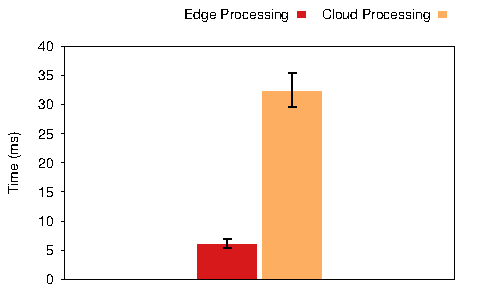
\includegraphics[width=0.8\textwidth]{Figures/Latency.pdf}
  \caption{Delay in processing a data element.} \label{fig:perf2}
\end{figure}
\begin{figure}[h]
  \centering
  	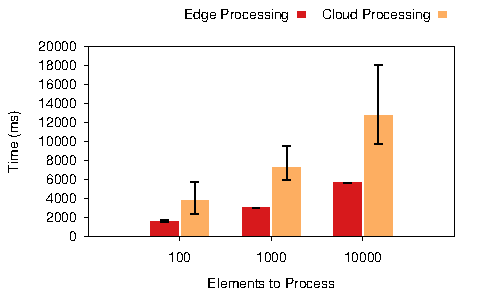
\includegraphics[width=0.8\textwidth]{Figures/EdgeVsCloud.pdf}
  \caption{Completion time for different workloads.} \label{fig:perf1}
\end{figure}

Figure~\ref{fig:perf2} shows the delay in processing a data element. The delay is measured as the time spent between the data producer generates the data element and the destination queue receives it for processing. We observe that in our case, the latency is up to 78\% less than a traditional approach consisting of sending data for processing to a cloud. The main reason is that our approach is able to dynamically identify different sources of computation and data using the location of the client. Therefore, it chooses to process the data in the place that is closest to the data source and the client. Our approach still incurs some small overheads as we have to identify the best processing site and data has to travel from source to destination. Nonetheless, these overheads are negligible compared with those incurred when transferring data between the edge and the core of the infrastructure.

Figure~\ref{fig:perf1} collects the computational time required to process a stream of data elements. We can observe that our approach is up to 56\% more efficient than a traditional cloud-based approach. In this particular case, this is directly related to the delay mentioned before that the system incurs when processing each data element. Since the delay of each data element is larger than its computational time, the system is often idle waiting for small periods of time until a new data element arrives.
\chapter{Application to the Distributed Operator Placement Problem}
\section{Introduction}

The number of Internet of Things applications is forecast to exponentially grow within the coming decade. Owners of such applications strive to make predictions from large streams of complex input in near real time. The heterogeneity among the edge devices and cloud servers introduces an important challenge for deciding how to split and orchestrate the IoT applications across the edge and the cloud. In this chapter, we propose a solution on how to split IoT applications dynamically across the edge and the cloud, allowing us to improve performance metrics such as end-to-end latency (response time), bandwidth consumption, and edge-to-cloud and cloud-to-edge messaging cost. 

%Cloud-based architectures often centralize storage and processing, generating high data movement overheads that penalize real-time applications. Edge and Cloud architecture pushes computation closer to where the data is generated, reducing the cost of data movements and improving the application response time. 

\section{Problem Description}
We focus on three performance metrics for placing \ac{IoT} applications across edge and cloud resources, \textit{i.e.}, the end-to-end application latency~\cite{daSilvaVeith:2018}, the WAN traffic, and the messaging cost (messages exchanged between the edge and the cloud). The \ac{IoT} operator placement problem consists of defining how to accommodate the application components (\textit{i.e.}, operators) on the available resources of the network topology to optimize one or more performance metrics. 

Table~\ref{tab:symbology} summarizes the notation used throughout the paper.
\begin{table}[ht]
  \centering
  \caption{Main notation adopted for the problem description.}
  \label{tab:symbology}
  \begin{tabular}{ll}
    \toprule
    Symbol & Description\\
    \midrule
    $\mathcal{R}$ & Set of cloud and edge resources\\
    $\mathcal{L}$ & Set of network links\\
    $i\!\leftrightarrow\!j$ & A link connecting resources $i$ and $j$ \\
    $cpu^r_i$, $mem^r_i$ & CPU and memory capacities of resource $i$ \\
    $lat_{i\!\leftrightarrow\!j}$,$bdw_{i\!\leftrightarrow\!j}$ & Latency and bandwidth of link $i\!\leftrightarrow\!j$ \\
    $\mathcal{O}$ & Set of stream processing operators \\
    $\mathcal{S}$ & Set of event streams between operators \\
%     $\mathcal{O}^{src}$, $\mathcal{O}^{out}$, $\mathcal{O}^{trn}$ & Sources, sinks and transformations \\  
    $f_i$ & Function to determine if the operator is a source, sink \\
    & and transformation\\
    $cpu^o_i$, $mem^o_i$ & CPU and memory req. of operator $i$\\
    $\psi^o_i$ & Selectivity of operator $i$\\
    $\omega^o_i$ & Data compression rate of operator $i$\\
    $s^{\rho}_{i\rightarrow j}$ & Probability that a message emitted\\ 
    &  by operator $i$ will flow to $j$\\ 
    $\lambda_i^{in},\lambda_i^{out}$ & Input/output event rate of operator $i$\\
    $\varsigma_i^{in},\varsigma_i^{out}$ & Input/output event size of operator $i$\\
    $stime_{\langle i,k\rangle}$ & Service time of operator $i$ at resource $k$\\
    $ctime_{\langle i,k\rangle\langle j,l\rangle}$ & Communication time from operator $i$ \\ 
    & at resource $k$ to $j$ at $l$ \\
%     $\varphi^{comp}_{\langle i,k\rangle}$ & Event service time of operator $i$\\
%     & at resource $k$\\ 
    $mem_{\langle i,k\rangle}$ & Overall memory required by operator\\
    &  $i$ when deployed at resource $k$\\
    $p_i, l_{p_i}$ & A graph path and its end-to-end latency\\ 
    $\mathcal{P}$ & The set of all paths in an application graph\\
    $\mu_{\langle i,k\rangle}$ & The rate at which operator $i$ \\
    & can process events at resource $k$\\
    \bottomrule
\end{tabular} 
\end{table}


We define a computational resource (\textit{i.e.}, cloud server or edge device) as a triple $ r_k = \langle cpu_k^r, mem_k^r, f_k^r\rangle \in\mathcal{R}$, where $cpu_k^r$ is the CPU capability in \ac{MIPS}, $mem_k^r$ is the memory capability in bytes, and $f_k^r\in\{0, 1\}$ signals whether $r_k$ is a \textit{cloud} resource. Similarly, the network link is drawn as a triple $l_{k\leftrightarrow l}=\langle bdw_{k\leftrightarrow l},lat_{k\leftrightarrow l}, f_{k\leftrightarrow l}\rangle\in\mathcal{L}$, where $k\leftrightarrow l$ represents the interconnection between resource $k$ and $l$, $bdw_{k\leftrightarrow l}$ the bandwidth capability in bits per second (bps), $lat_{k\leftrightarrow l}$ the latency in seconds, and $f_{k\leftrightarrow l}$ signals whether the link is part of a WAN. We consider the latency of a resource $k$ to itself (\textit{i.e} $lat_{k\leftrightarrow k}$) to be $0$.  

Each operator of the \ac{IoT} application is a quintuple $o_i = \langle cpu_i^o, mem_i^o, \psi_i^o, \omega_i^o, f_i\rangle\in\mathcal{O}$, where $cpu_i^o$ is the CPU requirement in \ac{IPS} to handle an individual event, $mem_i^o$ is the memory requirement in bytes to load the operator, $\psi_i^o$ is the ratio of number of input events to output events (\emph{i.e.}, selectivity), $\omega_i^o$ is the ratio of the size of input events to the size of output events (\emph{i.e.}, data compression/expansion factor), and $f_i\in\{source,sink,transformation\}$ signals whether $o_i$ is a \textit{source}, \textit{sink/output}, or \textit{transformation}. The rate at which operator $i$ can process events at resource $k$ is denoted by $\mu_{\langle i,k\rangle}$ and is essentially $\mu_{\langle i,k\rangle} = cpu_k^r\div cpu_i^o$. An event stream $s_{k\rightarrow l}^{\rho}\in\mathcal{S}$ connects operator $k$ to $l$ with a probability $\rho$ that an output event emitted by $k$ will flow through to $l$.

\begin{figure}
  \centering
  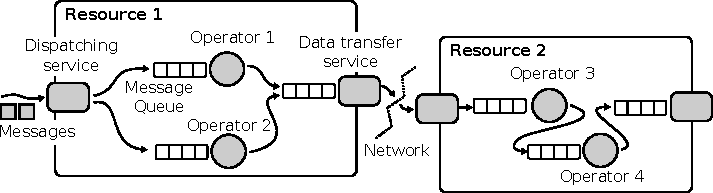
\includegraphics[width=1\columnwidth]{Figures/resource_model.pdf}
  \caption{Example of four operators and their respective queues placed on two resources.}
  \label{fig:deployment}
\end{figure}

The rate at which operator $i$ produces events is denoted by $\lambda_i^{out}$ and is a product of its input event rate $\lambda_i^{in}$ and its selectivity ($\psi^o_i$). The output event rate of a source operator ($f_k=source$) depends on the number of measurements it takes from a sensor or another monitored device. Likewise, we can recursively compute the average size $\varsigma_i^{in}$ of events that arrive at a downstream operator $i$ and the size of events it emits $\varsigma_i^{out}$ by considering the upstream operators' event sizes and their respective compression/expansion factors (\textit{i.e.}, $\omega^o_i$).

A computational resource can host one or more operators; operators within a same host communicate directly whereas inter-node communication is done via a communication service as depicted in Figure~\ref{fig:deployment}. Events are handled in a \ac{FCFS} fashion both by operators and the communication service that serialises messages to be sent to another host. Both operators and the communication service follow an M/M/1 model for their queues which allows for estimating the waiting and service times for computation and communication. The computation or service time $stime_{\langle o_i,r_k\rangle}$ of an operator $i$ placed on a resource $k$ is hence given by:

\begin{equation}
stime_{\langle i,k\rangle} = \frac{1}{\mu_{\langle i,k\rangle} - \lambda_{i}^{in}}
\label{eq:computation}
\end{equation}

\noindent while the communication time $ctime_{\langle i,k\rangle\langle j,l\rangle}$ for operator $i$ placed on a resource $k$ to send a message to operator $j$ on a resource $l$ is:
\begin{equation}
ctime_{\langle i,k\rangle\langle j,l\rangle} = \frac{1}{\Big(\frac{bdw_{k\leftrightarrow l}}{\varsigma_{i}^{out}}\Big) - \lambda_{j}^{in}} + l_{k\leftrightarrow l}
\label{eq:communication}
\end{equation}

A mapping function $\mathcal{M} : \mathcal{O} \rightarrow \mathcal{R}$, $\mathcal{S} \rightarrow \mathcal{L}$ indicates the resource to which an operator is assigned and the link(s) to which a stream is mapped. The function $mo_{\langle i,k\rangle}$ returns $1$ if operator $i$ is placed on resource $k$ and $0$ otherwise. Likewise, the function $ms_{\langle i\rightarrow j,k\leftrightarrow l\rangle}$ returns $1$ when the stream between operators $i$ and $j$ has been assigned to the link between resources $k$ and $l$, and $0$ otherwise.

A \textit{path} in the \ac{IoT} application graph is a sequence of operators from a source to a sink. A path $p_i$ of length $n$ is a sequence of $n$ operators and $n-1$ streams, starting at a source and ending at a sink:
\begin{equation}
p_i = o_{0},o_{1},\dots,o_{k},o_{k+1},\dots,o_{n-1}, o_{n} 
\end{equation}
  
Where $o_0=source$ and $o_n=sink$. The set of all possible paths in the application graph is denoted by $\mathcal{P}$. The end-to-end latency of a path comprises the sum of the computation time of all operators along the path and the communication time required to stream events on the path. More formally, the end-to-end latency of path $p_i$, denoted by $L_{p_i}$, is:


\begin{equation} \label{eq:latency}
  \begin{split}
  L_{p_i} =
  \sum_{\substack{o\in \mathcal{O} \\
                  r\in\mathcal{R}
                 }
        } 
   mo_{\langle o,r\rangle} \times stime_{\langle o,r\rangle} \\
   + \sum_{\substack{r'\in\mathcal{R}
                    }
         }    
   ms_{\langle o\rightarrow o+1,r\leftrightarrow r'\rangle} \times ctime_{\langle o, r\rangle\langle o+1,r'\rangle}      
  \end{split}   
\end{equation}

The WAN traffic accumulates the sizes of messages that cross the WAN network where $\mathbb{1}_{\{f_{k\leftrightarrow l} = 1\}}$ is the indicator that the link between the resource $k$ and $l$ is on a WAN. The WAN traffic of path $p_i$ is calculated as:
\begin{equation}
      W_{p_i} = \sum\limits_{
 \substack{s_{i\rightarrow j}\in\mathcal{S}\\
 k \leftrightarrow l\in\mathcal{L}
 }
 }{
    \mathbb{1}_{\{f_{k\leftrightarrow l} = 1\} } \times ms_{\langle i\rightarrow j,k\leftrightarrow l\rangle} \times \varsigma_i^{out}\quad 
 }
  \label{eq:traffic}
\end{equation}

Likewise, the messaging cost is calculated by the number of messages that reaches the cloud from the edge and vice versa. The indicator $\mathbb{1}_{ \{f_{k}^{r}=0\text{ and }f_{k^\prime}^{r} = 1\}}$ indicates that the previous operator $i$ is placed on edge ($f_{k}^r=0$) and it sends messages to operator $i^\prime$ in cloud ($f_{k^\prime}^{r} = 1$), the second part of the cost refers the other way cost (cloud to edge). The number of messages in $p_i$ is given as:
\begin{equation}
  \begin{split} 
    C_{p_i} = \smash{\sum_{\substack{i\in \mathcal{O} \\
                  i^\prime\in \mathcal{O} \\
                  k\in\mathcal{R} \\
                  k^\prime\in\mathcal{R}
                 }
          }      }
        \Big(\mathbb{1}_{ \{f_{k}^{r}=0\text{ and }f_{k^\prime}^{r} = 1\}}\times \big(mo_{\langle i^\prime,k^\prime\rangle} \times \\ \lambda_{i^\prime}^{in} + mo_{\langle i, k\rangle} \times\lambda_{i^\prime}^{out}\big) \Big)
  \end{split} 
  \label{eq:cost}
\end{equation}
\\

The parameters latency ($Par_{lat}$), WAN traffic ($Par_{wan}$), and monetary cost ($Par_{cost}$) receive the current values of the running application. A single aggregate cost metric uses the parameters and \textit{Simple Additive Weighting method} \cite{yoon:1995} (normalized in the interval [0,1]) offers a unified metric where $w_l$, $w_w$ and $w_c$, with $w_l + w_w + w_c = 1$, are non-negative weights for the different costs. Each metric of path $p_i$ is divided by its corresponding parameters and is then multiplied by its weight. The sum of the three metrics in the path $p_i$ results in the aggregate cost. Formally, the $AggregateCost$ in $p_i$ is determined as:


\begin{equation}
  \begin{split} 
    AggregateCost_{p_i} = w_l\times \frac{L_{p_i}}{Par_{lat}} + \\ w_w\times\frac{W_{p_i}}{Par_{wan}}+ w_c\times\frac{C_{p_i}}{Par_{cost}}
  \end{split}    
  \label{eq:placement}
\end{equation}

The problem of placing a distributed \ac{IoT} application consists of finding a mapping that minimizes the aggregate cost. % of all application paths and that respects the resource and network constraints. In other words, find the mapping that minimises the aggregate end-to-end event latency:

\begin{equation}
  \min \sum\limits_{p_i\in\mathcal{P}}{AggregateCost_{p_i}}
  \label{eq:objectivefunction}
\end{equation}
Subject to:
\begin{equation}
  \lambda_{o}^{in} < \mu_{\langle o,r\rangle} \quad\quad \forall o\in\mathcal{O}, \forall r\in\mathcal{R} | mo_{\langle o,r\rangle} = 1  
  \label{eq:comp_staturation}
\end{equation}
\begin{equation}
  \lambda_{o}^{in}<\Big(\frac{bdw_{k\leftrightarrow n}}{\varsigma_{o-1}^{out}}\Big) \quad\quad  \forall o\in\mathcal{O}, \forall k\!\leftrightarrow\!n\in\mathcal{L} |  mo_{\langle o,k\rangle} = 1 
    \label{eq:comm_staturation}
\end{equation}
\begin{equation}
 \sum_{o\in\mathcal{O}}mo_{\langle o,r\rangle}\times\lambda_{o}^{in} \le cpu_r \quad\quad \forall r\in\mathcal{R}
  \label{eq:comp_av}
\end{equation}
\begin{equation}
\sum _{o \in \mathcal{O}}
{
mo_{\langle o,r\rangle} \times mem_{\langle o,r\rangle} \le mem_{r} \quad\quad \forall r\in\mathcal{R}
}
   \label{eq:mem_av}
\end{equation}
\begin{equation}
 \sum\limits_{
 \substack{s_{i\rightarrow j}\in\mathcal{S}\\
 k \leftrightarrow l\in\mathcal{L}
 }
 }{
    ms_{\langle i\rightarrow j,k\leftrightarrow l\rangle} \times \varsigma_i^{out} \le bwd_{k \leftrightarrow l} \quad\quad \forall k \leftrightarrow l\in\mathcal{L}
 }
   \label{eq:comm_av}
\end{equation}
\begin{equation}
 \displaystyle \sum _{r \in \mathcal{R}} mo_{\langle o,r\rangle} = 1 \quad\quad \forall o \in \mathcal{O}
 \label{eq:vertex_map}
\end{equation}
\begin{equation}
 \sum\limits_{
 \substack{
%  s_{i\rightarrow j} \in \mathcal{S}\\
 k\leftrightarrow l \in \mathcal{L}}}
 {
 ms_{\langle i\rightarrow j,k\leftrightarrow l\rangle} = 1 \quad\quad \forall s_{i\rightarrow j} \in \mathcal{S}
 }
  \label{eq:edge_map}
\end{equation}

Constraint \ref{eq:comp_staturation} guarantees that a resource can provide the service rate required by its hosted operators whereas Constraint \ref{eq:comm_staturation} ensures that the links are not saturated. The CPU and memory requirements of operators on each host are ensured by Constraints~\ref{eq:comp_av} and \ref{eq:mem_av} respectively. Constraint~\ref{eq:comm_av} guarantees the data requirements of streams placed on links. Constraints \ref{eq:vertex_map} and \ref{eq:edge_map} ensure that an operator is not placed on more than a resource and that a stream is not placed on more than a network link respectively.

\section{R-Pulsar Framework Extension}\label{sec:framework}s
R-Pulsar has been extended with the following three components in order to automatically split and orchestrate dataflows between the edge and the cloud. 

\textbf{R-Pulsar Infrastructure Controller:} Designed to act similarly to software-defined networking (SDN) controllers, this component keeps track of the network resources available in real time. Some of the basic tasks include inventorying devices within the R-Pulsar P2P network, their capabilities, locations, and network statistics.

\textbf{R-Pulsar Plan Finder:} This component computes the most optimized operator placement plan. It uses a three-step approach for calculating the optimal operator placement plan for deploying dataflows between the edge and the cloud. Section~\ref{sec:strategies} presents the three-step operator placement strategy developed for R-Pulsar.

\textbf{R-Pulsar Executor/Monitor:} The primary responsibility is to monitor dataflows running on the R-Pulsar P2P network, including dataflow deployment, task assignment, and task reassignment in case of failure.

\subsection{R-Pulsar Nodes}

Each rendezvous point (RP) in the R-Pulsar P2P network can be elected as a master or as a worker. R-Pulsar differs from other master/slave clusters such as Apache Storm~\cite{storm} in the sense that R-Pulsar master and worker node roles are assigned dynamically every time a dataflow is deployed. 
\\\\
\textbf{Master RP:}
The master RP's primary responsibility is to manage, coordinate, and monitor a dataflow running on the R-Pulsar P2P network, including dataflow deployment, task assignment, and task reassignment in the event of a failure. Each time a new dataflow is deployed in the P2P network a new master RP for that dataflow is elected.

Deploying a topology to the R-Pulsar P2P network involves submitting the pre-packaged dataflow file along with topology configuration. Then the information will be routed to the responsible RP using the content-based interactions~\cite{Renart2018EdgeBD}. The content-based interactions allow users to route dataflows to unknown RPs; the RP who receives the message will be automatically elected as the master RP for that dataflow. Once the master RP has been elected, it then uses the infrastructure controller component to collect the network information of all the worker RPs. That information is then passed to the operator placement algorithm to generate a placement strategy. Once the operator placement algorithm has an efficient operator placement plan, then the master RP distributes the tasks to the worker RPs.

The master RP tracks the status of all worker nodes and the tasks assigned to each one. If the master RP detects that a specific worker node has failed to heartbeat or has become unavailable, it will reassign that worker RP tasks to other worker RP nodes in the federation.

The master RP is not a single point of failure in the strictest sense. This quality is because the master RP does not take part in the dataflow data processing, rather it merely manages the deployment, task assignment, and monitoring of the dataflow. In fact, if the master RP dies while a dataflow will continue to process data as long as the worker RPs assigned with tasks remain healthy. 

\textbf{Worker RP:} Each worker node is responsible for creating, starting, and stopping worker tasks assigned to that node. Worker RPs are also responsible for once the master RP has died to perform a master RP election.

\subsection{Placement Strategy}\label{sec:strategies}
The strategy for operator placement on R-Pulsar applies statistics collected by profiling the application and the location of sinks and sources. The operator placement aims to minimize the \textit{AggregateCost} (Equation~\ref{eq:objectivefunction}) by splitting the IoT application across edge and cloud by considering priorities of operators according to the infrastructure to which the sinks are assigned.
The operator placement strategy comprises three phases: (i) application profiling; (ii) candidate placement and (iii) final placement. 

\textbf{Phase 1 -- Application Profiling:}. 
In the first phase the worker RPs and the master RPs using the infrastructure controller component to continuously collect statistics~\cite{kaur:2017} from the running dataflow. The collected data includes the following information about the operators:
\begin{itemize}
  \item The arrival rate of events.
  \item Processing time per event.
  \item Number of MIPS required to process a tuple.
  \item Memory to run the operator.
  \item Arrival message size.
  \item Outcome message size.
\end{itemize}
This information is used to establish the selectivity, data compression/expansion factor, as well as, the CPU and memory requirements. 
\\
\\
\textbf{Phase 2 -- Candidate Placement:}
In phase two, the user-predefined locations of sinks and sources are used to identify patterns in the dataflow (Section~\ref{sec:api}). As depicted in Figure~\ref{fig:graph}, a dataflow can comprise multiple patterns such as (i) forks, where messages can be replicated to multiple downstream operators or scheduled to downstream operators in a round-robin fashion, using message key hashes, or considering other criteria \cite{Ni:2017}; (ii) parallel regions that perform the same operations over different sets of messages or where each individual region executes a given set of operations over replicas of the incoming messages; and (iii) joins, which merge the outcome of parallel regions. 

\begin{figure} 
  \centering
  \includegraphics[width=1\columnwidth]{Figures/patterns.pdf}
  \caption{Phases to determine the final placement using split points, where red means placed on edge, blue represents placed on cloud, and green delimits forks and joins.}
  \label{fig:graph}
\end{figure}

We consider that an IoT dataflow is a Series-Parallel-Decomposable Graph which either consists of a series of linearly dependent operators, or operators that can be executed independently in parallel, or a combination thereof. Phase 2 uses related techniques to identify graph regions that present these patterns \cite{Eidenbenz:2016}. This information is used to build a hierarchy of region dependencies (\textit{i.e.} downstream and upstream relations between regions) and assist in placing operators across cloud and edge resources. The streams in the graph paths that separate the operators are hereafter called the \textit{split points}. The rationale behind building such region hierarchy is to evaluate first the operators that can have greater impact on the overall end-to-end latency. Figure~\ref{fig:graph} illustrates the phases of the method to determine the split points (green circles), where red circles represent operators placed on edge resources whereas blue ones are on the cloud: (i) The method starts with sources and sinks whose placements are predefined by the user; (ii) split points are discovered (green circles) as well as sinks that correspond to actuators that can be placed on the edge; (iii) the branches between the existing patterns (green, red, and blue circles) are transformed into series regions; (iv) a hierarchy following the dependencies between regions is created; and (v) the regions provide information to split the operators on edge candidate placement evaluating if the operator flows events to actuators.

Algorithm~\ref{alg:patterns} describes the function $GetCandidates$ used to identify the patterns and obtain the series regions. First, the function adds two virtual vertices to the graph: $virt\_src$ connected to all data sources and $virt\_sink$ to which all sinks are connected (line~\ref{alg:patterns_virt_start}-\ref{alg:patterns_virt_end}). These vertices allow for recognizing all paths between sources and sinks. Second, each path is iterated moving operators to a temporary vector and classifying them as upstream and downstream according to the number of input and output edges (lines~\ref{alg:seriesregions_opdegree_begin}-\ref{alg:seriesregions_opdegree_downstream}). If the operator is a split point, the temporary vector is converted into a subset of regions set, and the temporary vector receives the current operator (lines~\ref{alg:seriesregions_opdegree_split}-\ref{alg:seriesregions_opdegree_addregions}). Third, the function removes the redundant values (line~\ref{alg:seriesregions_delete}). Fourth, the region set is iterated comparing the regions by the first and the last position values (equal values represent a connection) and consequently, they are stored in the hierarchy set (lines~\ref{alg:seriesregions_series_start}-\ref{alg:seriesregions_series_hier}). At last, using the hierarchy and the placement of the sinks, the function evaluates if the operator flows events to sinks placed on edge device then the operators is added to the $candidate$ lines~\ref{alg:begin_candidate_placement}-\ref{alg:end_candidate_placement}). 

\IncMargin{-0.4em} 
\RestyleAlgo{ruled}\LinesNumbered
\newcommand{\rand}{\emph{\textbf{and}}\xspace}
\newcommand{\ror}{\emph{\textbf{or}}\xspace}
\begin{algorithm}[ht]
\caption{Algorithm to get the candidate placement.}
\label{alg:patterns}
\DontPrintSemicolon
\SetAlgoLined
\SetAlgoVlined
\SetKwFunction{GetAllPaths}{GetAllPaths}
\SetKwFunction{SeriesRegions}{SeriesRegions}
\SetKwFunction{GetSinks}{GetSinks}
\SetKwFunction{GetLocation}{GetLocation}
\SetKwFunction{Break}{Break}
\SetKwProg{Fn}{Function}{}{}

\Fn{GetCandidates($\mathcal{G} = (\mathcal{O},\mathcal{S})$)}{
   $\mathcal{O} \gets \mathcal{O}\cup virt\_src\cup virt\_sink$\label{alg:patterns_virt_start}\; 

%    \For{$o\in \mathcal{O}^{src}$}{
      $\mathcal{S} \gets \mathcal{S} \cup s_{virt\_src \rightarrow o}, \forall o\in\mathcal{O}\text{ and } f_o=\text{source}$\;                       
%    }
%    $\mathcal{O} \gets \mathcal{O}\cup virt\_sink$\;
%    \For{$o\in \mathcal{O}^{out}$}{
      $\mathcal{S} \gets \mathcal{S} \cup s_{o \rightarrow virt\_sink}, \forall o\in\mathcal{O}\text{ and } f_o=\text{sink}$\label{alg:patterns_virt_end}\;  
%    }
%    $paths \gets $ \GetAllPaths{$\mathcal{G}, virt\_src, virt\_sink$}\label{alg:patterns_paths}\;
   
   
   
  %$temp \gets \{\}, regions \gets \{\}, hierarchy \gets \{\}$\label{alg:seriesregions_opdegree_start}\;
  \For{$p \in\text{ }$\GetAllPaths{$\mathcal{G}, virt\_src, virt\_sink$}}{\label{alg:seriesregions_opdegree_begin}
     \For{$o \in p$}{
%         \If{$(o\neq virt\_src$ \rand $o\neq virt\_sink)$}{
          $temp \gets temp\cup\{o\}, \forall o\not\in\{virt\_src,virt\_sink\}$\label{alg:seriesregions_opdegree_store}\;
%         }        
        $ups \gets |\langle *,o\rangle\subset\mathcal{S}|, downs \gets |\langle o,*\rangle\subset\mathcal{S}|$\label{alg:seriesregions_opdegree_downstream}\;
        
        \If{$ups >1$ \ror $downs >1$ \rand $ o\not\in\{virt\_src,virt\_sink\}$}{\label{alg:seriesregions_opdegree_split}
%           \If{$o \neq virt\_src$ \rand $o\neq virt\_sink $}{
              $regions \gets regions \cup temp,$ $temp \gets \{o\}$\label{alg:seriesregions_opdegree_addregions}\;
        %      $temp \gets \{o\}$\label{alg:seriesregions_opdegree_end}\;
%           }
        }
     }
  }
  Delete duplicate $regions$\label{alg:seriesregions_delete}\;
  \For{$src \in regions$}{\label{alg:seriesregions_series_start}
     \For{$dst \in regions$}{
        \If{$src \neq dst$}{\label{alg:seriesregions_series_end}
          \If{$src[|src|-1] = dst[0]$}{
             $hierarchy \gets hierarchy \cup \{src, dst\}$\label{alg:seriesregions_series_hier}\;
          }
        }
     }
  }
  
  
  \For{$operators \in regions$}{\label{alg:begin_candidate_placement}
     \For{$o \in operators$}{
       \If{$f_o\not\in\{source,sink\}$}{
          \For{$sink \in \GetSinks{$o$}$}{
            \If{\GetLocation{$sink$} = $edge$}{
              $candidate=candidate\cup o$\;
              \Break\; \label{alg:end_candidate_placement}
            }      
          }
       }  
    }
  }
  
    
  
  \Return{$candidate$}
}

\end{algorithm}

\textbf{Phase 3 -- Final Placement:} 
Once phase two has completed and the profiling phase has established the requirements from the different operators, an operator placement strategy is created and deployed. The strategy reduces the combinatorial space by estimating only once the computation (Equation~\ref{eq:computation}) and communication (Equation~\ref{eq:communication}) overheads to operators targeted to cloud (Phase 2). Otherwise, operators to edge (edge candiate placements) have their overheads estimated for all edge devices evaluating their constraints (Equation~\ref{eq:comp_staturation} --~Equation~\ref{eq:edge_map}). The strategy gives high priority to edge since cloud sinks often store messages for batch processing, whereas the edge side hosts actuators.
If edge devices cannot meet all operator requirements then the operator is moved to the cloud, hence, the cloud hosts its operator candidates and those that do not meet the constraints on edge. For instance, Operator 5 in Figure~\ref{fig:graph} was reallocated since the edge does not respect the resource constraints. Along with the overhead estimations, the strategy greedly uses the edge candiate placements for sequentially estimating the $AggregateCost$ (Equation~\ref{eq:placement}) and at each iteration, it picks the device with the minimal value (Equation~\ref{eq:objectivefunction}) to assign the operator.

\subsection{R-Pulsar API}
\label{sec:api}
In this section we present the API examples used for evaluating and deciding \textbf{how} to split the ETL dataflow, between the edge and the cloud resources. 

Listing~\ref{lst:place} is for specifying the operator constraints. In our case some of the operators need to be placed at the cloud and some others need to be placed at the edge. Note that if the wildcard or no placement is specified R-Pulsar will automatically decide the best placement for the operator. CloudTableInsert, MQTTPublish, and BloomFilterTask are tasks used in the ETL dataflow.

\begin{lstlisting}[ caption={User specified operator physical placements constraints.}, captionpos=b, label={lst:place}]
op1.map(CloudTableInsert()).placement(cloud);
op2.map(MQTTPublish()).placement(edge);
op3.map(BloomFilterTask()).placement(*);
\end{lstlisting}

Listing~\ref{lst:method} is for specifying the optimizations to apply to the dataflow. The R-Pulsar operator placement algorithm offers three optimizations: minimize end-to-end latency, bandwidth, or messaging cost. Each of the functions requires a weight normalized in the interval [0,1]; the sum of all three weights must be one. By doing so, users have the ability to optimize the latency, data transfer rate and messaging cost at the same time.

\begin{lstlisting}[caption={User specified dataflow optimizations (latency, data transfer rate and cost).}, captionpos=b, label={lst:method}]
topology.minEndToEndLatency(0.4);
topology.minDataTransferRate(0.3);
topology.minMessagingCost(0.3);
\end{lstlisting}

By specifying physical dataflow constraints and the optimizations desired R-Pulsar can obtain an optimal operator placement plan.  

\section{Evaluation}\label{sec:evaluation}
This section presents an experimental evaluation of our system. First, we present the setup and the other approaches in which the experiments will be evaluated and compared against. Second, we present an evaluation of our system based on latency, data transfer rate, and messaging cost. 

\subsection{Setup}

Our experiments are performed using the following edge and cloud setup:

\begin{itemize}

\item We used an experimental edge testbed developed by the authors, inspired by Hu \textit{et. al.}~\cite{Hu2016QuantifyingTI} that consists of 13 Raspberry Pis; 5 Raspberry Pis model 3 (4x ARM Cortex-A53 1.2GHz, 1GB of RAM and 10/100 Ethernet), and 8 Raspberry Pis model 2 (4x ARM Cortex-A7 900MHz, 1GB of RAM and 100 Ethernet). 

\item For the cloud we used the Chameleon cloud~\cite{chameleon} with 5 instances of type m1.medium (2 CPU and 4 GB RAM).

\end{itemize}

The 13 Raspberry Pis are connected to the same LAN. The Raspberry Pis use the external WAN~\cite{Ha:2013} (the Internet) for connecting to cloud. The LAN has a latency 0.523 ms and a bandwidth of 15 Mbits/sec. The WAN has latency 66.75 ms, and bandwidth of 87.0 Mbits/sec.

In addition to the setup, each of our experiments is evaluated using three other strategies. We compared our system with the following approaches:

\begin{itemize}	
\item \textbf{Cloud:} deploys all operators in the cloud, apart from operators provided in the initial placement.

\item \textbf{LB (Taneja et. al.~\cite{Taneja:2017}):} iterate a vector containing the application operators, gets the middle host of the computational vector, and evaluates CPU, memory, and bandwidth constraints to obtain the operator placement.

\item \textbf{Random:} simulates the user trying to guess the best placement for the dataflow between the edge and the cloud. Random is the average of 15 different dataflow deployments between the edge and the cloud resources.
\end{itemize}

All the tests are evaluated using the ETL dataflow. The ETL dataflow is an implementation of the ETL RIoTBench topology, it consists of: a single data source outputting data every 5 seconds, 2 sinks one located at the edge and one located at the cloud, and 7 tasks that need to be deployed between the edge and the cloud of the network. The experiments were conducted using Sense Your City dataset\footnote{http://map.datacanvas.org} which consists of transmitting data each minute from sensors in 7 cities across 3 continents, with about 12 sensors per city. The data content includes metadata on the sensor ID, geolocation, and five timestamped observations (outdoor temperature, humidity, ambient light, dust, and air quality).
\subsection{End-to-end Tuple Latency Evaluation}

The end-to-end tuple latency corresponds to the sum of the mean times from the two paths in ETL dataflow (cloud and edge). The conducted experiment evaluates the end-to-end tuple latency using Equation~\ref{eq:placement} where $w_l$ is equal to 1, and $w_w$ and $w_c$ are equal to 0. The experiment aims to evaluate how efficient the cloud, Random, and LB approaches are at minimizing the end-to-end tuple latency and compare the R-Pulsar operator placement approach. In addition, three failures were manually injected to showcase the dynamicity and flexibility to recover from node failures. The first failure makes 38\% of the edge cluster unavailable (100 ms). The second failure affects the remaining 62\% of the nodes (300 ms). Before the 62\% of the nodes fail, the 38\% of the nodes are back online. The third and last failure affects 50\% of the cloud instances (505 ms).

\begin{figure}[h!]
  \centering
  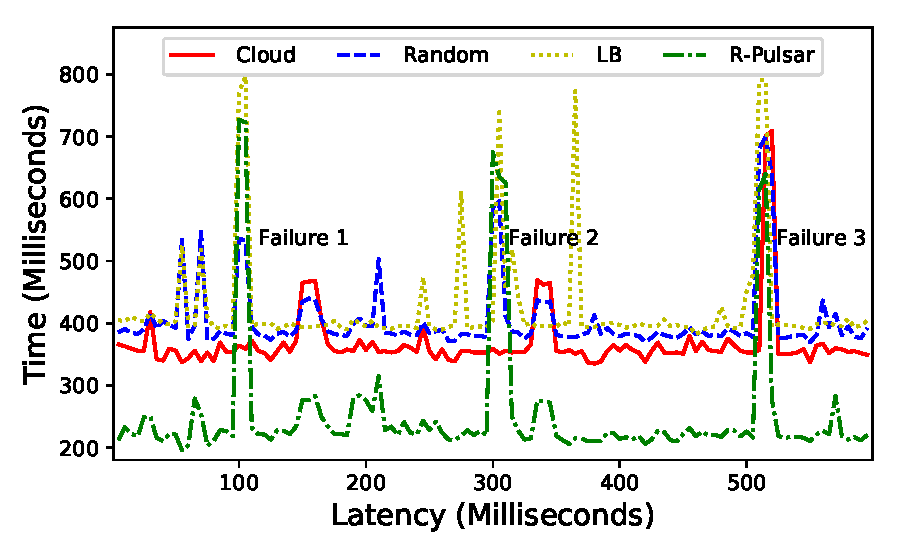
\includegraphics[width=0.8\textwidth]{Results/Latency.pdf}
  \caption{End-to-end tuple latency optimization with 3 self injected failures affecting edge and cloud nodes, while comparing it with Cloud, Random and LB approaches.}
  \label{fig:latency}
\end{figure} 

% \vspace{-2ex}

Figure~\ref{fig:latency} shows that on average tuples are computed 31\% faster when compared to the traditional cloud setup, and 38\% faster than Random and the LB placement approaches. The reason why the Random failures recover much faster than LB when compared to R-Pulsar is because Random is the average of multiple different deployments and in some cases the first failure is not affected. Figure~\ref{fig:latency} demonstrates that R-Pulsar operator placement strategy is capable of splitting the dataflow efficiently between the edge and the cloud and reduce the end-to-end tuple latency.

The second experiment aims to evaluate how efficient the Cloud, Random, and LB approaches are at minimizing end-to-end tuple latency and compare it with R-Pulsar approach. In this experiment no failures were injected.

\begin{figure}[h!]
  \centering
  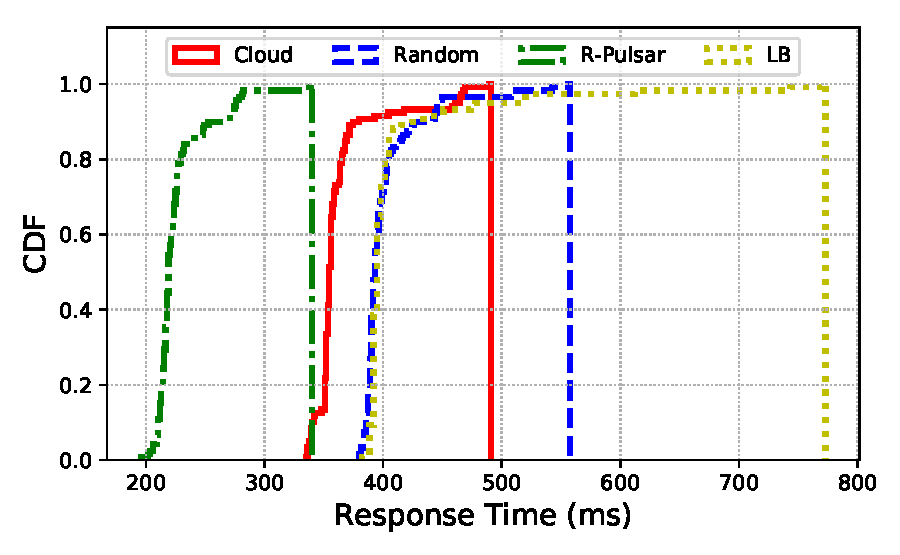
\includegraphics[width=0.8\textwidth]{Results/CDF_latency.pdf}
  \caption{End-to-end tuple latency optimization cumulative distribution function (CDF) comparison with Cloud, Random and LB approaches.}
  \label{fig:CDFLatency}
\end{figure} 

Figure~\ref{fig:CDFLatency} shows that when R-Pulsar operator placement approach is used 80\% of the tuples see a reduction in the end-to-end tuple latency by 44\% compared to the LB and Random approaches and 38\% compared to the cloud approach. 
 %R-Pulsar reduces the data transfers between the edge and the cloud by splitting the IoT application dataflow and by assigning operators to hosts to promote a better communication between themselves.

\subsection{Data Transfer Rate Evaluation}

The Data transfer rate consists of the sum of all message sizes that traverse a WAN link per second. The values for Equation~\ref{eq:placement} are $w_w$ equal to 1, and $w_l$ and $w_c$ equal to 0. This third experiment aims to evaluate how efficient are the cloud, Random, and LB approaches at minimizing the transfer rate between the edge and the cloud and compare the results with R-Pulsar operator placement approach. Minimizing the transfer rate between the edge and the cloud is a critical point in order to achieve real-time analytics. 

\begin{figure}
  \centering
  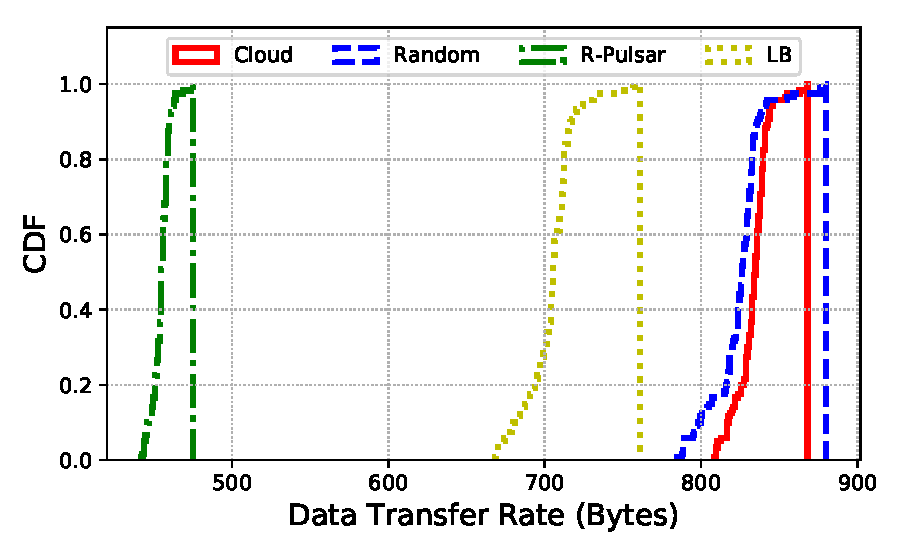
\includegraphics[width=0.8\textwidth]{Results/CDF_bandwidth.pdf}
  \caption{End-to-end data transfer rate optimization cumulative distribution function (CDF) comparison with cloud, Random and LB approaches.}
  \label{fig:bandwidth}
\end{figure} 


Figure~\ref{fig:bandwidth} shows that 80\% of the time R-Pulsar reduces the transfer rate between the edge and the cloud on average 35\% when compared to the LB approach. And it reduces the data transfer rate by 45\% when compared to the cloud and Random approaches.

This next experiment aims to evaluate the efficiency of minimizing the transfer rate and the end-to-end latency at the same time ($w_w$ = .5, $w_l$ = .5, and $w_c$ = 0). This experiment was also carried out using the cloud, Random, and LB approaches.

\begin{figure}
  \centering
  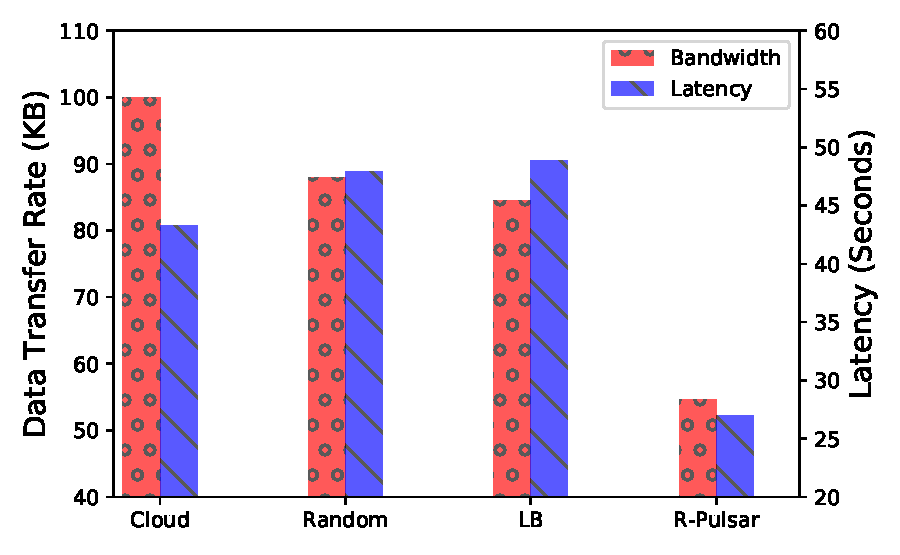
\includegraphics[width=0.8\textwidth]{Results/LandB.pdf}
  \caption{Multi optimization evaluation, end-to-end tuple latency and data transfer rate comparison with cloud, Random, and LB approaches.}
  \label{fig:both}
\end{figure} 

Figure~\ref{fig:both} shows that the R-Pulsar operator placement approach can also optimize the data transfer rate and the end-to-end latency by 46\% and 38\% respectively when compared to the cloud, 36\% and 45\% respectively when compared to the LB, 38\% and 44\% respectively when compared to the Random approach.

\subsection{Messaging Cost Evaluation}

This two experiments aim to calculate the messaging cost of running the dataflow for a month using the cost models of two major actors, AWS and Microsoft, in a real life edge and cloud scenario. For this reason, we setup Equation~\ref{eq:placement} with $w_c$ equal to 1, and $w_l$ and $w_l$ equal to 0. The goal of this optimization is to reduce the number of messages that reach the cloud servers.

\begin{table}[h]
\caption{Azure IoT Hub and Amazon IoT Core messaging pricing.} \label{tb:table}
\centering
\begin{tabular}{cc}
\toprule
Microsoft IoT Hub Pricing                                                               & AWS IoT Core Pricing                                                              \\ \toprule
\begin{tabular}[c]{@{}c@{}}Free Tier - 8,000 messages/day\\ \$0\end{tabular}        & \begin{tabular}[c]{@{}c@{}}Every 1 million messages/day\\ \$1.00\end{tabular} \\ \hline
\begin{tabular}[c]{@{}c@{}}Tier 1- 400,000 messages/day\\  \$25\end{tabular}        & \begin{tabular}[c]{@{}c@{}}Up to 1 billion messages/day\\ \$1.00\end{tabular} \\ \hline
\begin{tabular}[c]{@{}c@{}}Tier 2 - 6,000,000 messages/day \\  \$250\end{tabular}   & \begin{tabular}[c]{@{}c@{}}Next 4 billion messages/day\\ \$0.80\end{tabular}  \\ \hline
\begin{tabular}[c]{@{}c@{}}Tier 3 - 300,000,000 messages/day\\ \$2,500\end{tabular} & \begin{tabular}[c]{@{}c@{}}Over 5 billion messages/day\\ \$0.70\end{tabular}  \\ \bottomrule
\end{tabular}
\end{table}

Table~\ref{tb:table} depicts two IoT cost models. The first cost model is the Microsoft Azure IoT Hub~\cite{HubPricing}. Each tier enables a maximum number of messages exchanged between the Azure IoT Edge and the Azure IoT Hub and vice versa per day. T1 allows up to 400,000 messages a day, T2 allows up to 6,000,000 messages a day, and T3 allows up to 300,000,000 messages a day. 

The second cost model is the Amazon IoT Core~\cite{AWSPricing} where messaging is metered by the number of messages transmitted between your devices and AWS IoT Core and vice versa per day. Amazon offers multiple costs for different regions, for this experiment we choose the cheapest region (N.Virginia) which charges \$1 per million messages sent, and the cost per message decreases after the first 1 billion messages per day.

\begin{figure}[h!]
  \centering
  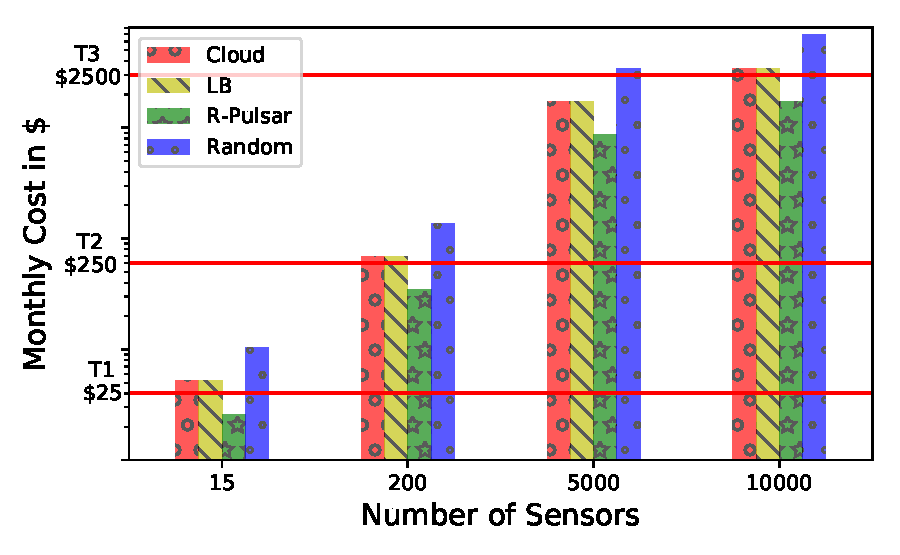
\includegraphics[width=0.8\textwidth]{Results/Cost_Microsoft.pdf}
  \caption{Messaging cost savings evaluation based on the Microsoft Azure IoT Hub pricing model, for four different setups.}
  \label{fig:cost-microsoft}
\end{figure} 

% \vspace{-2ex}

Figure~\ref{fig:cost-microsoft} depicts the cost of deploying the ETL dataflow using the Microsoft cost model using the four different approaches presented earlier. When using a small setup (15 sensors), the monthly cost for our system will be \$25 a month while the cloud, LB, or Random approaches will cost \$250 a month, savings of 90\%. A similar behavior happens with a medium (200 sensors) and extra large (10000 sensors) setups. 

\begin{figure}[h!]
  \centering
  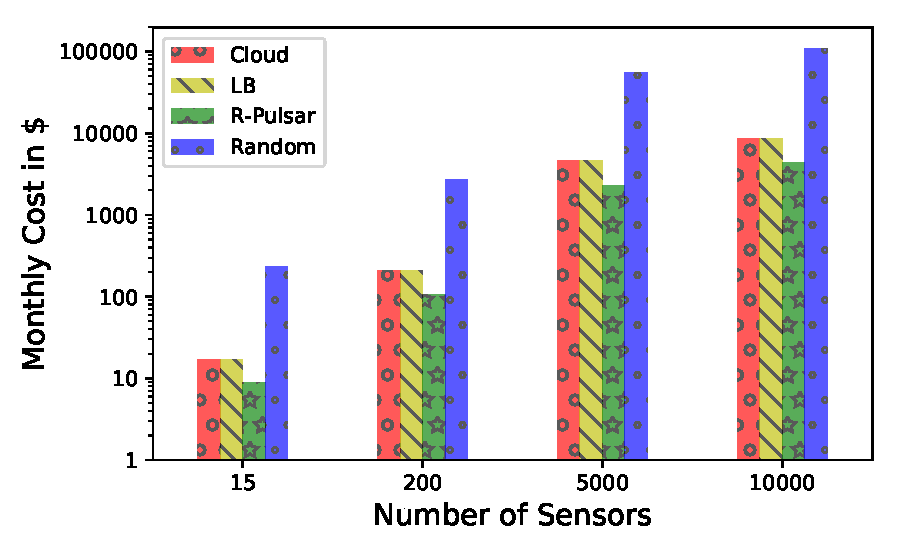
\includegraphics[width=0.8\textwidth]{Results/Cost_Amazon.pdf}
  \caption{Messaging cost savings evaluation based on the Amazon IoT pricing model, for four different setups.}
  \label{fig:cost-amazon}
\end{figure} 


Figure~\ref{fig:cost-amazon} depicts the cost of deploying the ETL dataflow using the Amazon cost model. Our system obtains a 50\% cost reduction when compared to the cloud and LB approaches in all four different setups (15, 200, 5000 and 10000 sensors). In addition our system obtains a 97\% savings when compared to the Random approach in all four different setups.

\subsection{Model Evaluation}

This last three experiments aim to evaluate the scalability, overhead and validate the operator placement algorithm.

\begin{figure}[h]
  \centering
  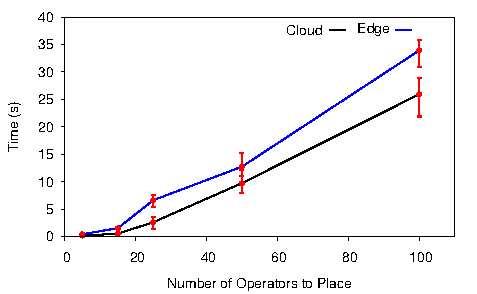
\includegraphics[width=0.8\textwidth]{Results/Scale.pdf}
  \caption{Evaluation of the scalability of the operator placement problem algorithm as the number of operators to place increase over edge and cloud resources.}\label{fig:scalefirst}
\end{figure}

Figure~\ref{fig:scalefirst} depicts the scalability and the overhead of the initial operator placement problem algorithm in both edge and cloud resources. We can observe that the algorithm scales with the number of operators to place and a valid solution can be found in less than half a minute. Not that this step is only performed when the entire workflow needs to be placed, once the operators are placed, only a portion of the operators are moved.

\begin{figure}[h]
  \centering
  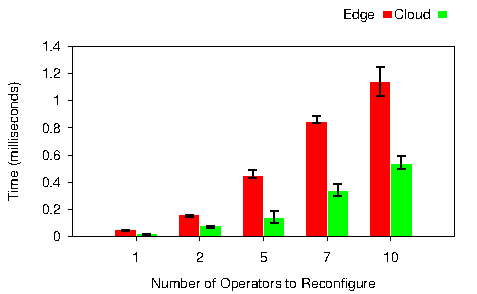
\includegraphics[width=0.8\textwidth]{Results/Redeploy.pdf}
  \caption{Evaluation of the cost of redeploying a subset of operators over edge and cloud resources.}\label{fig:scalesecond}
\end{figure}

Figure~\ref{fig:scalefirst} depicts the redeployment scalability and overhead of the algorithm. We can observer that since we do not need to redeploy all the operators when the workflow is not meeting the constraints, we can see that the cost of redeploying a subset of operators is very low and more important decisions can be done in real time since it the redeployment calculations are small.

\begin{figure}[h]
  \centering
  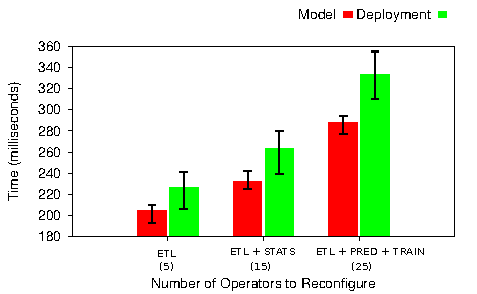
\includegraphics[width=0.8\textwidth]{Results/Time.pdf}
  \caption{Evaluation of the real-time vs the modeled time as the number of operators increases.}\label{fig:validation} 
\end{figure}

The final result we wanted to validate the model by comparing the expected results and the actual results after deploying the workflow in a real setup, Figure~\ref{fig:validation} depicts the results. We can observe that when the number of operators is small the difference between the expected and the actual results only differs by at most 10\%, when the number of operators grows to 25 the difference slightly grows up to 15\%.

\chapter{Conclusion and Future Work}
\section{Conclusion}
This thesis identified and addressed key problems and requirements of IoT applications. Specifically, this thesis presented a programming abstraction enables to address the what, where, and when data needs to be processed by specifying content and action descriptors. In addition this thesis also tackles the how to split a given dataflow and place operators across edge and cloud resources. First, presented a modification of the Associative Rendezvous programming abstraction to allow to decide what and where data needs to be processed. Second presented a R-Pulsar an IoT Edge Framework that extends cloud capabilities to edge devices, enabling users to collect and analyze data closer to the source of the information. Third presented a rule-based programming abstraction for specifying when to trigger data-processing tasks based on data observations. Finally, presented a solution to the distributed operator placement problem for allowing to decide how to split the application operators between the edge and the cloud, by specifying a set of constraints. We evaluated the effectiveness, scalability, performance and overheads of R-Pulsar software stack by using three sets of IoT applications and validated every layer by performing scalability, overhead and performance tests.

\section{Perspectives}
The research presented in this dissertation opens several research problems that need to be addressed in order to further advance on the edge computing area.
\\\\
\textbf{Energy Management:} A study published in 2017 determined that due to the large number of IoT devices connected to the internet by 2025 they will consume 20\% of all the worldwide electricity consuption~\cite{Energy}. For those reasons there is a need to implement energy management policies.  Energy management needs to be incorporated in the service layer in order to be able to schedule computations based on the energy consumption. A large amount of research exists focused on modeling and optimizing the energy consumption in the Cloud, but there is limited research targeting edge computing.  R-Pulsar does not have the ability to quantify the amount of energy spend or to schedule computations while being energy efficient. There is a need for tools that will give feedback on how energy efficient the code is. For those reasons energy management is a potential research direction.
\\\\
\textbf{Security and Privacy:} IoT data differentiates itself from any other type of data due that is mostly built upon personal and highly sensitive data. For those reasons security is an important research topic. There is a need for algorithms that provide strong security guarantees, while still being suitable for constrained environments. R-Pulsar does not address any security or privacy cancers, so a possible research direction is to create algorithms that provide strong security protection, while fitting within an acceptable footprint. It needs to be lightweight enough that will still leave room for the embedded OS and applications code. 
\\\\
\textbf{Edge based stream processing engines:} There is a need to develop more lightweight stream processing engine that can be deployed on constrained devices. Current stream processing engines (SPEs) such as Storm~\cite{storm}, Flink~\cite{flink}, Heron~\cite{heron} and Spark~\cite{spark} where designed to be deployed in the Cloud, with large number of clusters with powerful computing resources and plenty of memory. However, these assumptions do not hold at the Edge of the network. R-Pulsar does not offer a new SPE, it just simply uses Apache Edgent. For this reason there is a need to research a develop new SPE that are designed to run in constrained devices.


\bibliographystyle{ieeetr}
\bibliography{References}

%\begin{vita}
%\heading{The author of my thesis} \vspace{15pt}
% Colleges attended, with dates, subjects, degrees
%\begin{descriptionlist}{xxxxx-xxxxx} % reverse chronological order
%\item[200x] Ph. D. in Computer Science, Rutgers University
%\item[200x-0x] B. Sc. in Computer Science from some University
%\item[200x] Graduated from such and such high school.
%\end{descriptionlist}
%\medskip
%\begin{descriptionlist}{xxxxx-xxxxx} %positions held since BS degree
%\item[200x-200y] Teaching assistant, Department of Computer Science, Rutgers University
%\end{descriptionlist}
%\end{vita}

\end{document}
